\documentclass[a4paper,10pt,twoside,openany]{book}

\usepackage[lang=hebrew]{maths}
\usepackage{polynom}
\usepackage{hebrewdoc}
\usepackage{stylish}
\usepackage{lipsum}
\let\bs\blacksquare

\setlength{\parindent}{0pt}

%%%%%%%%%%%%
% Styling %
%%%%%%%%%%%%

\usepackage{enumitem}

%%%%%%%%%%%%%
% Counters  %
%%%%%%%%%%%%%

\setcounter{section}{1}     
            
%BIBLIOGRAPHY
\usepackage[
backend=biber,
style=alphabetic,
]{biblatex}
\addbibresource{bibliography.bib} %Imports bibliography file

\title{
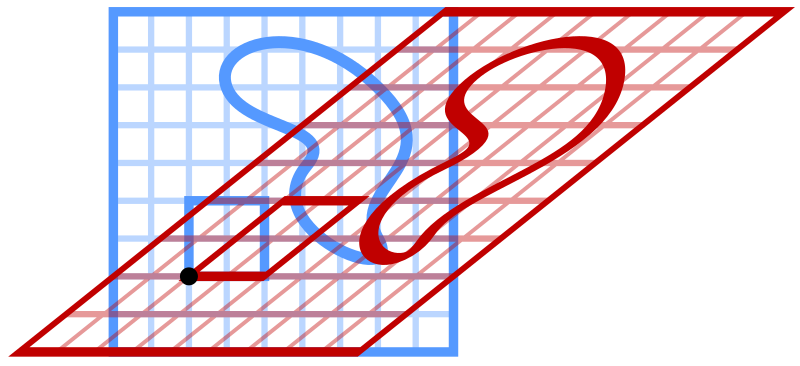
\includegraphics[width=6in]{images/front.png}\\
\vspace{30pt}
\Huge
אלגברה ב' (01040168)
\\
אביב 2025
\\
רשימות תרגולים
\vspace{30pt}
\\
\huge
אלן סורני
\vspace{30pt}
\\
\Large
הרשימות עודכנו לאחרונה בתאריך ה־%
\today
}
\date{}

\begin{document}
\frontmatter
\maketitle
\tableofcontents

\mainmatter

\section*{סימונים}

\begin{itemize}
\item[-]
$\brs{n} = \set{1, \ldots, n}$.
\item[-]
$\sum_{i \in \brs{n}} a_i = \sum_{i=1}^n a_i = a_1 + a_2 + \ldots + a_n$
\item[-] $\Mat_{m \times n}\prs{\mbb{F}}$ הוא מרחב המטריצות עם
$m$
שורות ו־%
$n$
עמודות, עם מקדמים בשדה
$\mbb{F}$.
\item[-]
$\mbb{F}^n = \Mat_{n \times 1}\prs{\mbb{F}}$
\item[-]
$\Mat_{n}\prs{\mbb{F}} = \Mat_{n \times n}\prs{\mbb{F}}$
\item[-]
$\hom_{\mbb{F}}\prs{V,W}$
הוא מרחב ההעתקות הלינאריות
$V \to W$
כאשר
$V,W$
מרחבים וקטוריים מעל
$\mbb{F}$.
\item[-]
$\End_{\mbb{F}}\prs{V} = \hom_{\mbb{F}}\prs{V,V}$
\end{itemize}

\part{חלק ראשון - מרחבים שמורים}

\chapter{חזרה על מטריצות מייצגות}

\section{הגדרות ותכונות בסיסיות}

\begin{definition}[וקטור קואורדינטות]
יהי
$V$
מרחב וקטורי סוף־מימדי מעל שדה
$\mbb{F}$,
יהי
$B = \prs{v_1, \ldots, v_n}$
בסיס של
$V$
ויהי
$v \in V$.
\emph{וקטור הקואורדינטות של
$v$
לפי הבסיס
$B$}
הוא הוקטור
$\brs{v}_B = \pmat{\alpha_1 \\ \vdots \\ \alpha_n}$
כאשר
$\alpha_1, \ldots, \alpha_n \in \mbb{F}$
היחידים עבורם
\[\text{.}v = \sum_{i \in [n]} \alpha_i v_i \coloneqq \alpha_1 v_1 + \ldots + \alpha_n v_n\]
\end{definition}

\begin{remark}
ההעתקה
\begin{align*}
\rho_B \colon V &\to \mbb{F}^n \\
v &\mapsto \brs{v}_B
\end{align*}
היא איזומורפיזם לינארי.
\end{remark}

\begin{definition}[מטריצה מייצגת]
יהיו
$V,W$
מרחבים וקטורים סוף־מימדיים מעל אותו שדה
$\mbb{F}$
עם בסיסים
$B,C$
בהתאמה, ונסמן
\[\text{.} B = \prs{v_1, \ldots, v_n}\]
נסמן גם
$n \coloneqq \dim\prs{V}$
ו־%
$m \coloneqq \dim\prs{W}$.
עבור
$T \in \Hom_{\mbb{F}}\prs{V,W}$
נגדיר
\[\text{.} \brs{T}^B_C = \pmat{\vert & & \vert \\ \brs{T\prs{v_1}}_C & \cdots & \brs{T\prs{v_n}}_C \\ \vert & & \vert} \in \Mat_{m \times n}\prs{\mbb{F}}\]
\end{definition}

\begin{theorem}[כפל מטריצות]
תהי
$A \in \Mat_{m \times n}\prs{\mbb{F}}$
ויהי
$E = \prs{e_1, \ldots, e_m}$
הבסיס הסטנדרטי של
$\mbb{F}^n$.
אז:
\begin{enumerate}[label = (\roman*)]
\item
לכל
$i \in [m]$
מתקיים כי
$A e_i$
העמודה ה־%
$i$
של
$A$.
\item
לכל
$B = \pmat{\vert & & \vert \\ b_1 & \cdots & b_\ell \\ \vert & & \vert} \in \Mat_{n \times \ell}\prs{\mbb{F}}$
מתקיים
$AB = \pmat{\vert & & \vert \\ A b_1 & \cdots & A b_\ell \\ \vert & & \vert}$.
\end{enumerate}
\end{theorem}

\begin{exercisechap}
הראו שניתן לשחזר את ההגדרה של כפל מטריצות משתי התכונות במשפט.
\end{exercisechap}

\begin{remark}
ההעתקה
\begin{align*}
\eta^B_C \colon \Hom_{\mbb{F}}\prs{V,B} &\to \Mat_{m \times n}\prs{\mbb{F}} \\
T &\mapsto \brs{T}^B_C
\end{align*}
היא איזומורפיזם לינארי.
\end{remark}

\begin{proposition}
תהי
$T \in \Hom_{\mbb{F}}\prs{V,W}$
ויהיו
$B = \prs{v_1, \ldots, v_n}$
בסיס של
$V$
ו־%
$C$
בסיס של
$W$.
אז
\[\brs{T}^B_C \brs{v}_B = \brs{T\prs{v}}_C\]
לכל
$v \in V$.
\end{proposition}

\begin{notation}
אם
$B$
בסיס של מרחב וקטורי סוף־מימדי
$V$
ואם
$T \in \End\prs{V}$,
נסמן
$\brs{T}_B \coloneqq \brs{T}^B_B$
ונקרא למטריצה זאת
\emph{המטריצה המייצגת של
$T$
לפי הבסיס
$B$}.
\end{notation}

\begin{notation}
יהי
$V$
מרחב וקטורי סוף־מימדי עם בסיסים
$B,C$.
נסמן
$M^B_C \coloneqq \brs{\id_V}^B_C$.
\end{notation}

\begin{notation}
אם
$A \in \Mat_{n\times n}\prs{\mbb{F}}$,
נסמן
\begin{align*}
T_A \colon \mbb{F}^n &\to \mbb{F}^n \\
\text{.} \hphantom{lalala} v &\mapsto Av
\end{align*}
\end{notation}

\section{תרגילים}

\begin{exercisechap}\label{ex:p(x+1)}
יהי
$V = \mbb{R}_3\brs{x}$
מרחב הפולינום הממשיים ממעלה לכל היותר
$3$,
תהי
\begin{align*}
T \colon \mbb{R}_3\brs{x} &\to \mbb{R}_3\brs{x} \\
p\prs{x} &\mapsto p\prs{x+1}
\end{align*}
ויהי
$B = \prs{1,x,x^2,x^3}$
בסיס של
$V$.
כיתבו את
$\brs{T}_B$.
\end{exercisechap}

\begin{solution}
לפי הגדרת המטריצה המייצגת,
עמודות
$\brs{T}_B$
הן
$\brs{T\prs{x^i}}_B$
עבור
$i \in \set{0,1,2,3}$.
מתקיים
\begin{align*}
T\prs{1} &= 1 \\
T\prs{x} &= x+1 = 1 + x \\
T\prs{x^2} &= \prs{x+1}^2 = 1 + 2x + x^2 \\
T\prs{x^3} &= \prs{x+1}^3 = 1 + 3x + 3x^2 + x^3
\end{align*}
ולכן
\begin{align*}
\brs{T\prs{1}}_B &= e_1 \\
\brs{T\prs{x}}_B &= e_1 + e_2 \\
\brs{T\prs{x^2}}_B &= e_1 + 2 e_2 + e_3 \\
\brs{T\prs{x^3}}_B &= e_1 + 3 e_2 + 3 e_3 + e_4
\end{align*}
ואז
\begin{align*}
\text{.} \brs{T}_B &= \pmat{1 & 1 & 1 & 1 \\ 0 & 1 & 2 & 3 \\ 0 & 0 & 1 & 3 \\ 0 & 0 & 0 & 1}
\end{align*}
\end{solution}

\begin{exercisechap}
יהי
$V = \Mat_{2 \times 2}\prs{\mbb{C}}$,
תהי
\begin{align*}
T \colon V &\to V \\
A &\mapsto \frac{1}{2} \prs{A - A^t}
\end{align*}
ויהי
\[E = \prs{E_{1,1}, E_{1,2}, E_{2,1}, E_{2,2}} \coloneqq \pmat{\pmat{1 & 0 \\ 0 & 0}, \pmat{0 & 1 \\ 0 & 0}, \pmat{0 & 0 \\ 1 & 0}, \pmat{0 & 0 \\ 0 & 1}}\]
\emph{הבסיס הסטנדרטי של
$V$}.
כיתבו את
$\brs{T}_E$.
\end{exercisechap}

\begin{solution}
כמו מקודם, נחשב את
$\brs{T\prs{E_{i,j}}}_E$
כיוון שאלו עמודות
$\brs{T}_E$.
מתקיים
\begin{align*}
T\prs{E_{1,1}} &= \frac{1}{2} \prs{E_{1,1} - E_{1,1}} = 0 \\
T\prs{E_{1,2}} &= \frac{1}{2} \prs{\pmat{0 & 1 \\ 0 & 0} - \pmat{0 & 0 \\ 1 & 0}} = \frac{1}{2} E_{1,2} - \frac{1}{2} E_{2,1} \\
T\prs{E_{2,1}} &= \frac{1}{2} \prs{E_{2,1} - E_{1,2}} = \frac{1}{2} E_{2,1} - \frac{1}{2} E_{1,2} \\
\text{,} T\prs{E_{2,2}} &= \frac{1}{2} \prs{E_{2,2} - E_{2,2}} = 0 \\
\end{align*}
לכן
\begin{align*}
\brs{T\prs{E_{1,1}}}_E &= 0 \\
\brs{T\prs{E_{1,2}}}_E &= \frac{1}{2} e_2 - \frac{1}{2} e_3 \\
\brs{T\prs{E_{2,1}}}_E &= -\frac{1}{2} e_2 + \frac{1}{2} e_3 \\
\brs{T\prs{E_{2,2}}}_E &= 0
\end{align*}
ואז
\begin{align*}
\text{,} \brs{T}_E &= \pmat{0 & 0 & 0 & 0 \\ 0 & \frac{1}{2} & -\frac{1}{2} & 0 \\ 0 & -\frac{1}{2} & \frac{1}{2} & 0 \\ 0 & 0 & 0 & 0}
\end{align*}
כנדרש.
\end{solution}

\begin{exercisechap}
יהי
$V = \Hom_{\mbb{R}}\prs{\mbb{R}^2, \mbb{R}}$
עם הבסיס
$B = \prs{f_1, f_2}$
כאשר
\begin{align*}
f_1\prs{\pmat{x \\ y}} &= x \\
\text{,} f_2\prs{\pmat{x \\ y}} &= y
\end{align*}
ותהי
\begin{align*}
\text{.} A &= \pmat{1 & 2 \\ 3 & 4} \in \Mat_{2 \times 2}\prs{\mbb{R}}
\end{align*}
מיצאו
$T \in \End_{\mbb{R}}\prs{V}$
עבורו
$\brs{T}_B = A$.
\end{exercisechap}

\begin{solution}
עבור
$T \in \End_{\mbb{R}}\prs{V}$
מתקיים
\[\text{.} \brs{T}_B = \pmat{\vert & \vert \\ \brs{T\prs{f_1}}_B & \brs{T\prs{f_2}}_B \\ \vert & \vert}\]
לכן נדרוש
\begin{align*}
\brs{T\prs{f_1}}_B &= \pmat{1 \\ 2} \\
\text{.} \brs{T\prs{f_2}}_B &= \pmat{3 \\ 4}
\end{align*}
אז
\begin{align*}
T\prs{f_1} &= f_1 + 2 f_2 \\
\text{.} T\prs{f_2} &= 3 f_1 + 4 f_2
\end{align*}
לכן, אם
$f \in V$
איבר כללי, נכתוב
\[f\pmat{x\\y} = \alpha x + \beta y = \alpha f_1 \pmat{x \\ y} + \beta f_2\pmat{x \\ y}\]
ונקבל כי
\begin{align*}
\prs{T\prs{f}}\pmat{x\\y} &= \prs{T\prs{\alpha f_1 + \beta f_2}}\pmat{x\\y}
\\&= \alpha T\prs{f_1}\pmat{x\\y} + \beta T\prs{f_2} \pmat{x\\y}
\\&= \alpha \prs{f_1 + 2 f_2}\pmat{x\\y} + \beta \prs{3 f_1 + 4 f_2} \pmat{x\\y}
\\ \text{.} \hphantom{\prs{T\prs{f}}\pmat{x\\y}} &= \alpha \prs{x + 2 y} + \beta \prs{3 x + 4y}
\end{align*}
\end{solution}

\begin{exercisechap}
תהיינה
$A,B \in \Mat_{m \times n}\prs{\mbb{F}}$
ונניח כי לכל
$v \in \mbb{F}^n$
מתקיים
$Av = Bv$.
אז
$A = B$.
\end{exercisechap}

\begin{solution}
מהנתון, מתקיים
$\prs{A - B}v = 0$
לכל
$v \in \mbb{F}^n$.
בפרט העמודה ה־%
$i$
של
$A-B$,
שהינה
$\prs{A - B}e_i$,
שווה ל־%
$0$.
לכן
$A - B = 0$.
\end{solution}

\begin{proposition}
יהיו
$U,V,W$
מרחבים וקטוריים סוף־מימדיים מעל אותו שדה
$\mbb{F}$
עם בסיסים
$B,C,D$
בהתאמה,
ותהיינה
\begin{align*}
S \in \Hom_{\mbb{F}}\prs{U,V} \\
\text{.} T \in \Hom_{\mbb{F}}\prs{V,W}
\end{align*}
אז
\[\text{.} \brs{T \circ S}^B_D = \brs{T}^C_D \brs{S}^B_C\]
\end{proposition}

\begin{exercisechap} \label{exercisechap:change-of-basis-through-isomorphism}
יהיו
$V,W$
מרחבים וקטוריים סוף־מימדיים מעל שדה
$\mbb{F}$
ותהי
$T \in \Hom_{\mbb{F}}\prs{V,W}$
חד־חד ערכית.

יהיו
\begin{align*}
B &= \prs{v_1, \ldots, v_n} \\
C &= \prs{u_1, \ldots, u_n}
\end{align*}
בסיסים של
$V$
ויהיו
\begin{align*}
B' &= \prs{T\prs{v_1}, \ldots, T\prs{v_n}} \\
\text{.} C' &= \prs{T\prs{u_1}, \ldots, T\prs{u_n}}
\end{align*}
אז
$B',C'$
בסיסים של
$\im\prs{T} = \set{T\prs{v}}{v \in V}$
וגם
$M^B_C = M^{B'}_{C'}$.
\end{exercisechap}

\begin{solution}
כיוון ש־%
$T$
חד־חד ערכית ועל התמונה, צמצום הטווח נותן איזומורפיזם
$T \colon V \riso \im\prs{T}$.
איזומורפיזם שולח בסיס לבסיס, לכן
$B',C'$
בסיסים.

כעת, לכל
$i \in [n]$
נכתוב
\begin{align*}
v_i &= \sum_{j \in \brs{n}} \alpha_{i,j} u_i
\end{align*}
ואז
\begin{align*}
\text{.} M^B_C e_i = \brs{v_i}_C = \pmat{\alpha_{i,1} \\ \vdots \\ \alpha_{i,n}}
\end{align*}
כמו כן,
\begin{align*}
T\prs{v_i}
&=
T\prs{\sum_{i \in [n]} \alpha_{i,j} u_j}
\\&=
\sum_{i \in [n]} \alpha_{i,j} T\prs{u_j}
\end{align*}
ולכן גם
\[\text{.} M^{B'}_{C'} e_i = \brs{T\prs{v_i}}_{C'} = \pmat{\alpha_{i,1} \\ \vdots \\ \alpha_{i,n}}\]
קיבלנו כי כל עמודות המטריצות שוות, ולכן יש שוויון.
\end{solution}

\begin{exercisechap}
תהי
$A \in \Mat_{n \times n}\prs{\mbb{F}}$
הפיכה.
\begin{enumerate}
\item יהי
$E$
הבסיס הסטנדרטי של
$\mbb{F}^n$.
מיצאו בסיס
$B$
של
$\mbb{F}^n$
עבורו
$A = M^B_E$.

\item
מיצאו בסיס
$C$
של
$\mbb{F}^n$
עבורו
$A = M^E_C$.

\item \emph{
(לא הספקנו בתרגול)
}
יהי
$B$
בסיס של
$\mbb{F}^n$.
מיצאו בסיס
$C$
של
$\mbb{F}^n$
עבורו
$A = M^B_C$.

\item \emph{
(לא הספקנו בתרגול)
}
יהי
$V$
מרחב וקטורי ממימד
$n \in \mbb{N}_+$
מעל
$\mbb{F}$,
יהי
$T \in \End_{\mbb{F}}\prs{V}$
איזומורפיזם
ויהי
$B = \prs{v_1, \ldots, v_n}$
בסיס של
$V$.
מיצאו בסיס
$C$
של
$V$
עבורו
$\brs{T}^B_C = A$.
\end{enumerate}
\end{exercisechap}

\begin{solution}
\begin{enumerate}
\item
אם
$B = \prs{v_1, \ldots, v_n}$,
מתקיים מההגדרה כי
\[\text{.} M^B_E = \pmat{\vert & & \vert \\ \brs{v_1}_E & \cdots & \brs{v_n}_E \\ \vert & & \vert} = \pmat{\vert & & \vert \\ v_1 & \cdots & v_n \\ \vert & & \vert}\]
לכן ניקח את
$\prs{v_1, \ldots, v_n}$
להיות עמודות
$A$,
לפי הסדר.

\item
לכל
$v \in \mbb{F}^n$
מתקיים
\[M^C_E M^E_C v = M^C_E \brs{v}_C = \brs{v}_E = v\]
ולכן
$M^E_C = \prs{M^C_E}^{-1}$.
אם ניקח
$C = \prs{u_1, \ldots, u_n}$
כאשר
$u_i$
העמודה ה־%
$i$
של
$A^{-1}$
נקבל מהסעיף הקודם כי
$M^C_E = A^{-1}$
ולכן
$M^E_C = \prs{A^{-1}}^{-1} = A$.
כלומר ניקח,
$u_i = A^{-1} e_i$.

\item
מתקיים
$M^B_C = M^E_C M^B_E$
לכן נרצה שיתקיים
$M^E_C M^B_E = A$
או במילים אחרות
$M^E_C = A \prs{M^B_E}^{-1} = A M^E_B$.
מהסעיף הקודם, נרצה
$C = \prs{u_1, \ldots, u_n}$
כאשר
$u_i$
העמודה ה־%
$i$
של
$\prs{A M^E_B}^{-1} = M^B_E A^{-1}$,
כלומר
\[\text{.} u_i = M^B_E A^{-1} e_i\]

\item
עבור כל בסיס
$C'$
מתקיים
$\brs{T}^B_{C'} = M^B_{C'} \brs{T}^B_B$
לכן נרצה
$M^B_C \brs{T}^B_B = A$.
כיוון ש־%
$T$
איזומורפיזם, המטריצה
$\brs{T}^B_B$
הפיכה, ולכן נרצה
$M^B_C = A \prs{\brs{T}^B_B}^{-1}$.
כעת, אם
$C = \prs{v_1, \ldots, v_n}$
נקבל לפי
\ref{proposition:change-of-basis-through-isomorphism}
עבור האיזומורפיזם
$\rho_B$
כי
$M^B_C = M^E_{\hat{C}}$
כאשר
$\hat{C} = \prs{\brs{v_1}_B, \ldots, \brs{v_n}_B}$.
לכן נחפש
$\hat{C}$
עבורו
$M^E_{\hat{C}} = A \brs{T}_B^{-1}$.
לפי הסעיף השני, נרצה
$\hat{C} = \prs{u_1, \ldots, u_n}$
עבור
\[\text{.} u_i = \prs{A \brs{T}_B^{-1}}^{-1} e_i = \brs{T}_B A^{-1} e_i\]
לכן
\[\text{.} v_i = \rho_B^{-1} \prs{\brs{T}_B A^{-1} e_i}\]
\end{enumerate}
\end{solution}

\begin{exercisechap}[לא הספקנו בתרגול]
יהי
$V = \mbb{C}_3\brs{x}$,
תהי
\begin{align*}
T \colon V &\to V \\
\text{,} \hphantom{lalala} p\prs{x} &\mapsto p\prs{x+1}
\end{align*}
יהי
$E = \pmat{1,x,x^2,x^3}$,
\emph{הבסיס הסטנדרטי}
ותהי
$A = \pmat{0 & 1 & 0 & 0 \\ 1 & 0 & 0 & 0 \\ 0 & 0 & 0 & 1 \\ 0 & 0 & 1 & 0}$.
כיתבו מפורשות בסיס
$C$
של
$V$
עבורו
$A = \brs{T}^E_C$.
\end{exercisechap}

\begin{solution}
לפי התרגיל הקודם, נרצה קודם
$\hat{C} = \prs{u_1, \ldots, u_4}$
כאשר
$u_i = \brs{T}_E A^{-1} e_i$.
חישבנו ב־%
\ref{ex:p(x+1)}
כי
\[\brs{T}_E = \pmat{1 & 1 & 1 & 1 \\ 0 & 1 & 2 & 3 \\ 0 & 0 & 1 & 3 \\ 0 & 0 & 0 & 1}\]
וניתן לראות כי
$A^2 = I$
כלומר
$A^{-1} = A$.
נשים לב כי
\begin{align*}
A e_1 &= e_2 \\
A e_2 &= e_1 \\
A e_3 &= e_4 \\
A e_4 &= e_3
\end{align*}
ואז נקבל
\begin{align*}
u_1 &= \brs{T}_E A^{-1} e_1 = \brs{T}_E e_2 = \pmat{1 \\ 1 \\ 0 \\ 0} \\
u_2 &= \brs{T}_E A^{-1} e_2 = \brs{T}_E e_1 = \pmat{1 \\ 0 \\ 0 \\ 0} \\
u_3 &= \brs{T}_E A^{-1} e_3 = \brs{T}_E e_4 = \pmat{1 \\ 3 \\ 3 \\ 1} \\
\text{,} u_4 &= \brs{T}_E A^{-1} e_4 = \brs{T}_E e_3 = \pmat{1 \\ 2 \\ 1 \\ 0}
\end{align*}
כלומר
\[\text{,} \hat{C} = \prs{\pmat{1 \\ 1 \\ 0 \\ 0}, \pmat{1 \\ 0 \\ 0 \\ 0}, \pmat{1 \\ 3 \\ 3 \\ 1}, \pmat{1 \\ 2 \\ 1 \\ 0}}\]
ולבסוף
\[\text{.} C = \prs{v_1, v_2, v_3, v_4} \coloneqq \prs{1+x, 1, 1+3x+3x^2+x^3, 1+2x+x^2}\]

ליתר ביטחון, נבדוק שהמטריצה המייצגת היא אכן
$A$.
מתקיים
\begin{align*}
T\prs{1} &= 1 = v_2 \\
T\prs{x} &= x+1 = v_1 \\
T\prs{x^2} &= \prs{x+1}^2 = 1+2x+x^2 = v_4 \\
T\prs{x^3} &= \prs{x+1}^3 = 1+3x+3x^2+x^3 = v_3
\end{align*}
ולכן
\begin{align*}
\brs{T}^E_C &= \pmat{\vert & \vert & \vert & \vert \\ \brs{T\prs{1}}_C & \brs{T\prs{x}}_C & \brs{T\prs{x^2}}_C & \brs{T\prs{x^3}}_C \\ \vert & \vert & \vert & \vert}
\\&= \pmat{\vert & \vert & \vert & \vert \\ \brs{v_2}_C & \brs{v_1}_C & \brs{v_4}_C & \brs{v_3}_C \\ \vert & \vert & \vert & \vert}
\\&= \pmat{\vert & \vert & \vert & \vert \\ e_2 & e_1 & e_4 & e_3 \\ \vert & \vert & \vert & \vert}
\\&= A
\end{align*}
כנדרש.
\end{solution}

\chapter{הדטרמיננטה}

\section{הגדרות ותכונות בסיסיות}

\begin{definition}[דטרמיננטה]
תהי
$A \in \Mat_{n \times n}\prs{\mbb{F}}$
מטריצה עם מקדמים בשדה
$\mbb{F}$.
נגדיר את
\emph{הדטרמיננטה}
$\det\prs{A}$
של
$A$
באופן הרקורסיבי הבא.

תהי
$A_{\prs{i,j}}$
המטריצה המתקבלת מ־%
$A$
על ידי הסרת השורה ה־%
$i$
והעמודה ה־%
$j$.
המספר
$\det\prs{A_{\prs{i,j}}}$
נקרא
\emph{המינור}
ה־$\prs{i,j}$ של
$A$
והדטרמיננטה של
$A$
שווה
\begin{align*}
\det\prs{A} &= \sum_{i \in \brs{n}} \prs{-1}^{i+j} a_{i,j} \det\prs{A_{\prs{i,j}}}
\end{align*}
עבור כל
$j \in \brs{n}$
קבוע, ושווה
\begin{align*}
\det\prs{A} &= \sum_{j \in \brs{n}} \prs{-1}^{i+j} a_{i,j} \det\prs{A_{\prs{i,j}}}
\end{align*}
עבור כל
$i \in \brs{n}$
קבוע.
\end{definition}

\begin{theorem}
תהיינה
$A, B, C \in \Mat_{n \times n}\prs{\mbb{F}}$
ונניח כי
$C$
הפיכה.
מתקיימות התכונות הבאות.
\begin{enumerate}
\item $\det\prs{AB} = \det\prs{A} \cdot \det\prs{B}$
\item $\det\prs{C^{-1}} = \prs{\det\prs{C}}^{-1}$
\end{enumerate}
\end{theorem}

\begin{theorem}
\begin{enumerate}
\item החלפת שתי שורות או עמודות במטריצה כופלת את הדטרמיננטה ב־%
$\prs{-1}$.
\item כפל שורה או עמודה במטריצה בסקלר
$\alpha$
כופל את הדטרמיננטה ב־%
$\alpha$.
\item הוספת כפולה שורה או עמודה לשורה או עמודה במטריצה אינה משנה את הדטרמיננטה.
\end{enumerate}
\end{theorem}

\section{תרגילים}

\begin{exercisechap}
חשבו את הדטרמיננטות של המטריצות הבאות.

\begin{enumerate}
\item \[\pmat{1 & 2 & 3 \\ 4 & 5 & 6 \\ 7 & 8 & 9} \in \Mat_{3}\prs{\mbb{R}}\]
\item \[\pmat{0 & 0 & 0 & 1 \\ 0 & 0 & 1 & 0 \\ 0 & 1 & 0 & 0 \\ 1 & 0 & 0 & 0} \in \Mat_{4}\prs{\mbb{R}}\]
\item \[\pmat{1 & 0 & 0 \\ 0 & 1 & 0 \\ 1 & 1 & 1} \in \Mat_{3}\prs{\mbb{R}}\]
\item \[\pmat{1 & 0 & 1 \\ 0 & 1 & 0 \\ 1 & 1 & 1} \in \Mat_{3}\prs{\mbb{R}}\]
\end{enumerate}
\end{exercisechap}

\begin{solution}
\begin{enumerate}
\item
נחשב לפי השורה הראשונה.
\begin{align*}
\det \pmat{1 & 2 & 3 \\ 4 & 5 & 6 \\ 7 & 8 & 9} &= 1 \cdot \det\pmat{5 & 6 \\ 8 & 9} - 2 \cdot \det \pmat{4 & 6 \\ 7 & 9} + 3 \cdot \det \pmat{4 & 5 \\ 7 & 8}
\\&=
1 \cdot \prs{5 \cdot 9 - 6 \cdot 8} - 2 \cdot \prs{4 \cdot 9 - 6 \cdot 7} + 3 \cdot \prs{4 \cdot 8 - 5 \cdot 7}
\\&=
1 \cdot \prs{-3} -2 \cdot \prs{-6} + 3 \cdot \prs{-3}
\\&=
-3 + 12 - 9
\\&= 0
\end{align*}
\item החלפת שורות כופלת את הדטרמיננטה ב־%
$\prs{-1}$.
כיוון שניתן לקבל את המטריצה ממטריצת היחידה על ידי החלפת השורות
$1,4$
והשורות
$2,3$,
נקבל כי הדטרמיננטה שווה לזאת של היחידה. לכן
\[\text{.} \det \pmat{0 & 0 & 0 & 1 \\ 0 & 0 & 1 & 0 \\ 0 & 1 & 0 & 0 \\ 1 & 0 & 0 & 0} = 1\]
\item
הוספת כפולה של השורות הראשונה והשנייה ב־%
$\prs{-1}$
לשורה השלישית לא משנה את הדרמיננטה. לכן הדטמיננטה של המטריצה שווה לזאת של היחידה, ולכן
\[\text{.} \det \pmat{1 & 0 & 0 \\ 0 & 1 & 0 \\ 1 & 1 & 1} = 1\]
\item
הוספת כפולה של השורות הראשונה והשנייה ב־%
$\prs{-1}$
לשורה השלישית לא משנה את הדרמיננטה. לכן הדטמיננטה של המטריצה שווה לזאת של
\begin{align*}
\text{.} \pmat{1 & 0 & 1 \\ 0 & 1 & 0 \\ 0 & 0 & 0}
\end{align*}
כיוון שהשורה השלישית היא שורת אפסים, אם נפתח את הדטרמיננטה לפיה נקבל שהדטרמיננטה שווה
$0$.
זה נכון באופן כללי יותר אם השורות תלויות לינארית, כי נוכל לקבל שורת אפסים מצירוף לינארי של השורות.
\end{enumerate}
\end{solution}

\begin{exercisechap}
תהי
$T \in \End_{\mbb{F}}\prs{V}$
העתקה לינארית ויהי
$B$
בסיס של
$V$.
הראו כי ניתן להגדיר
$\det\prs{T} = \det\prs{\brs{T}_B}$.
כלומר, הראו שאם
$C$
בסיס נוסף של
$V$
מתקיים
$\det\prs{\brs{T}_B} = \det\prs{\brs{T}_C}$.
\end{exercisechap}

\begin{solution}
מתקיים
\begin{align*}
\brs{T}_B = \prs{M^B_C}^{-1} \brs{T}_C M^B_C
\end{align*}
ולכן
\begin{align*}
\text{.} \det\prs{\brs{T}_B} &= \det\prs{\prs{M^B_C}^{-1}} \det\prs{\brs{T}_C} \det\prs{M^B_C}
\end{align*}
כיוון ש־%
$\det\prs{A^{-1}} = \frac{1}{\det\prs{A}}$
 לכל מטריצה
 $A$,
 מתקיים
 $\det\prs{\prs{M^B_C}^{-1}} = \frac{1}{\det\prs{M^B_C}}$.
 לכן, נקבל בסה"כ כי
 \[\text{,} \det\prs{\brs{T}_B} = \det\prs{\brs{T}_C}\]
 כנדרש.
\end{solution}

\section{הדטרמיננטה לפי תמורות}

\begin{notation}
נסמן תמורה
$\sigma \in S_n$
בתור
$\sigma = \prs{\sigma\prs{1}, \ldots, \sigma\prs{n}}$,
וחילוף
$\tau$
בין איברים
$n,m$
בתור
$\prs{n;m}$.
\end{notation}

\begin{proposition}
תהי
$A = \prs{a_{i,j}}_{i,j \in \brs{n}} \in \Mat_n\prs{\mbb{F}}$.
מתקיים
\[\text{.} \det\prs{A} = \sum_{\sigma \in S_n} \sgn{\sigma} \prod_{i \in \brs{n}} a_{i,\sigma\prs{i}}\]
\end{proposition}

\begin{exercisechap}
חשבו את הדטרמיננטה של המטריצה הבאה לפי תמורות.

\begin{align*}
\text{.} A = \pmat{1 & 2 & 3 \\ 4 & 5 & 6 \\ 7 & 8 & 9}
\end{align*}
\end{exercisechap}

\begin{solution}
נרשום את כל איברי
$S_3$.
הם
\begin{align*}
\id_{S_3} = \prs{1, 2, 3}, \\
\prs{1, 3, 2}, \\
\prs{2, 1, 3}, \\
\prs{2, 3, 1}, \\
\prs{3, 1, 2}, \\
\text{.} \prs{3, 2, 1}
\end{align*}
עבור כל אחד מהאיברים, נפעיל חילופים משמאל כדי להביא אותו ליחידה, ומספר החילופים יהיה החזקה של $\prs{-1}$ בסימן של התמורה. אם הגענו לתמורה קודמת, מספר החילופים שנותרו משלב זה הוא מספר החילופים שכבר מצאנו בחישוב קודם.
\begin{align*}
\id_{S_3} = \id_{S_3} &\implies \sgn\prs{\id_{S_3}} = 1\\
\prs{2;3} \circ \prs{\prs{1, 3, 2}} = \prs{\prs{1, 2, 3}} = \id_{S_3} &\implies \sgn\prs{\prs{1, 3, 2}} = -1 \\
\prs{1;2} \circ \prs{\prs{2, 1, 3}} = \prs{\prs{1, 2, 3}} = \id_{S_3} &\implies \sgn\prs{\prs{2,1,3}} = -1 \\
\prs{1;2} \circ \prs{\prs{2, 3, 1}} = \prs{\prs{1, 3, 2}} &\implies \sgn\prs{\prs{2, 3, 1}} = -1 \cdot \sgn\prs{\prs{1, 3, 2}} = 1 \\
\prs{1;3} \circ \prs{\prs{3, 1, 2}} = \prs{\prs{1, 3, 2}} &\implies \sgn\prs{\prs{3, 1, 2}} = \prs{-1} \cdot \sgn\prs{\prs{1, 3, 2}} = 1 \\
\text{.} \prs{1;3} \circ \prs{\prs{3,2,1}} = \prs{\prs{1,2,3}} = \id_{S_3} &\implies \sgn\prs{\prs{3,2,1}} = -1
\end{align*}

לכן נקבל
\begin{align*}
\det\prs{A} &= 1\cdot 5 \cdot 9 - 1 \cdot 6 \cdot 8 - 2 \cdot 4 \cdot 9 + 2 \cdot 6 \cdot 7 + 3 \cdot 4 \cdot 8 - 3 \cdot 5 \cdot 7
\\&= 45 - 48 - 72 + 84 + 96 - 105
\\ \text{.} \hphantom{\det\prs{A}} &= 0
\end{align*}
\end{solution}

\chapter{המטריצה המצורפת וכלל קרמר}

\section{הגדרות ותכונות בסיסיות}

\begin{definition}[המטריצה המצורפת]
תהי
$A \in \Mat_{n}\prs{\mbb{F}}$.
\emph{המטריצה המצורפת של
$A$}
היא המטריצה
$\adj\prs{A} \in \Mat_n\prs{\mbb{F}}$
המקיימת
\begin{align*}
\text{.} \adj\prs{A}_{i,j} = \prs{-1}^{i+j} \det\prs{A_{\prs{j,i}}}
\end{align*}
\end{definition}

\begin{proposition}
עבור
$A \in\Mat_n\prs{\mbb{F}}$
מתקיים
\begin{align*}
\text{.} A \adj\prs{A} = \adj\prs{A} A = \det\prs{A} I_n
\end{align*}
\end{proposition}

\begin{corollary}
עבור
$A \in \Mat_n\prs{\mbb{F}}$
הפיכה מתקיים
\begin{align*}
\text{.} A^{-1} = \frac{1}{\det\prs{A}} \adj\prs{A}
\end{align*}
\end{corollary}

\begin{theorem}[כלל קרמר]
תהי
$A \in \Mat_n\prs{\mbb{F}}$
הפיכה, ויהי
$b \in \mbb{F}^n$.
עבור כל
$i \in\brs{n}$,
נסמן ב־%
$A_i$
את המטריצה המתקבלת על ידי החלפת העמודה ה־%
$i$
של
$A$
ב־%
$b$.
אז, למשוואה
$Ax = b$
קיים פתרון יחיד
$x \coloneqq \prs{x_i}_{i \in \brs{n}} \in \mbb{F}^n$
הנתון על ידי
\begin{align*}
\text{.} \forall i \in \brs{n} \colon x_i = \frac{\det\prs{A_i}}{\det\prs{A}}
\end{align*}
\end{theorem}

\section{תרגילים}

\begin{exercisechap}
תהי
$A = \pmat{1 & -1 & 2 \\ 2 & 3 & 5 \\ -2 & 0 & 1} \in \Mat_3\prs{\mbb{R}}$.
חשבו את
$\adj\prs{A}$.
\end{exercisechap}

\begin{solution}
נחשב את
$\adj\prs{A}$
לפי ההגדרה.
\begin{align*}
\adj\prs{A} &= \pmat{\det\pmat{3 & 5 \\ 0 & 1} & -\det\pmat{-1 & 2 \\ 0 & 1} & \det\pmat{-1 & 2 \\ 3 & 5} \\
-\det\pmat{2 & 5 \\ -2 & 1} & \det\pmat{1 & 2 \\ -2 & 1} & -\det\pmat{1 & 2 \\ 2 & 5} \\
\det\pmat{2 & 3 \\ -2 & 0} & -\det\pmat{1 & -1 \\ -2 & 0} & \det\pmat{1 & -1 \\ 2 & 3}}
\\&=
\pmat{3 & 1 & -11 \\ -12 & 5 & -1 \\ 6 & 2 & 5}
\end{align*}
\end{solution}

\begin{exercisechap}
היעזרו במטריצה המצורפת כדי לחשב את ההופכית עבור כל אחת מהמטריצות הבאות.

\begin{align*}
A &= \pmat{-2 & 3 & 2 \\ 6 & 0 & 3 \\ 4 & 1 & -1} \in \Mat_3\prs{\mbb{R}} \\
B &= \pmat{\cos{\theta} & 0 & -\sin{\theta} \\
0 & 1 & 0 \\
\sin{\theta} & 0 & \cos{\theta}} \in \Mat_3\prs{\mbb{R}}
\end{align*}
עבור
$\theta \in \mbb{R}$.
\end{exercisechap}

\begin{solution}
עבור כל אחת משתי המטריצות, נחשב את הדטרמיננטה ואת המטריצה המצורפת שלה.
מתקיים
\begin{align*}
\det\prs{A} &= -2 \det\pmat{0 & 3 \\ 1 & -1} - 3 \det\pmat{6 & 3 \\ 4 & -1} + 2 \det\pmat{6 & 0 \\ 4 & 1}
\\&= -2 \cdot \prs{-3} - 3 \cdot \prs{-18} + 2 \cdot 6
\\&= 72 \\
\det\prs{B} &= 0 + 1 \cdot \det\pmat{\cos{\theta} & -\sin{\theta} \\ \sin{\theta} & \cos{\theta}} - 0
\\&= \cos^2{\theta} + \sin^2{\theta}
\\&= 1
\end{align*}
וכן
\begin{align*}
\adj\prs{A} &= \pmat{\det\pmat{0 & 3 \\ 1 & -1} & -\det\pmat{6 & 3 \\ 4 & -1} & \det\pmat{6 & 0 \\ 4 & 1} \\
-\det\pmat{3 & 2 \\ 1 & -1} & \det\pmat{-2 & 2 \\ 4 & -1} & -\det\pmat{-2 & 3 \\ 4 & 1} \\
\det\pmat{3 & 2 \\ 0 & 3} & -\det\pmat{-2 & 2 \\ 6 & 3} & \det\pmat{-2 & 3 \\ 6 & 0}}^t
\\&= \pmat{-3 & 18 & 6 \\ 5 & -6 & 14 \\ 9 & 18 & -18}^t
\\&= \pmat{-3 & 5 & 9 \\ 18 & -6 & 18 \\ 6 & 14 & -18} \\
\adj\prs{B} &= \pmat{
\det\pmat{1 & 0 \\ 0 & \cos\theta} & -\det\pmat{0 & 0 \\ \sin \theta & \cos \theta} & \det\pmat{0 & 1 \\ \sin\theta & 0} \\
-\det\pmat{0 & - \sin\theta \\ 0 & \cos\theta} & \det\pmat{\cos \theta & - \sin \theta \\ \sin\theta & \cos\theta} & -\det\pmat{\cos \theta & 0 \\ \sin \theta & 0} \\
\det\pmat{0 & -\sin\theta \\ 1 & 0} & -\det\pmat{\cos \theta & - \sin \theta \\ 0 & 0} & \det\pmat{\cos\theta & 0 \\ 0 & 1}}^t
\\&=
\pmat{\cos\theta & 0 & -\sin\theta \\ 0 & 1 & 0 \\ \sin \theta & 0 & \cos \theta}^t
\\&=
\pmat{\cos\theta & 0 & \sin\theta \\ 0 & 1 & 0 \\ -\sin \theta & 0 & \cos \theta}
\end{align*}
ולכן נקבל כי
\begin{align*}
A^{-1} &= \frac{1}{\det\prs{A}} \adj\prs{A}
\\&= \frac{1}{72} \pmat{-3 & 5 & 9 \\ 18 & -6 & 18 \\ 6 & 14 & -18}
\\&= \pmat{-1/24 & 5/72 & 1/8 \\ 1/4 & -1/12 & 1/4 \\ 1/12 & 7/36 & -1/4} \\
B^{-1} &= \frac{1}{\det\prs{B}} \adj\prs{B}
\\\text{,} \hphantom{B^{-1}} &= \pmat{\cos\theta & 0 & \sin\theta \\ 0 & 1 & 0 \\ -\sin \theta & 0 & \cos \theta}
\end{align*}
כנדרש.
\end{solution}

\begin{exercisechap}
תהי
$A \in \Mat_n\prs{\mbb{F}}$
הפיכה.
הראו כי
$\adj\prs{\adj\prs{A}} = \det\prs{A}^{n-2} A$.
\end{exercisechap}

\begin{solution}
\begin{description}
\item[דרך 1:]
$A$
הפיכה, לכן
$\adj\prs{A} = \det\prs{A} A^{-1}$
גם היא הפיכה. לפי אותה נוסחה נקבל כי
\begin{align*}
\adj\prs{\adj\prs{A}} &= \det\prs{\adj\prs{A}} \adj\prs{A}^{-1} \\
\\&= \frac{\det\prs{\adj\prs{A}}}{\det\prs{A}} A
\end{align*}
ולכן נותר להראות כי
\begin{align*}
\text{.} \det\prs{\adj\prs{A}} = \det\prs{A}^{n-1}
\end{align*}
אכן
\begin{align*}
\det\prs{\adj\prs{A}} &= \det\prs{\det\prs{A} A^{-1}}
\\&= \det\prs{A}^n \det\prs{A^{-1}}
\\\text{,}\hphantom{\det\prs{\adj\prs{A}}}&= \det\prs{A}^{n-1}
\end{align*}
כנדרש.

\item[דרך 2:]
$A$
הפיכה, לכן
$\adj\prs{A} = \det\prs{A} A^{-1}$
גם היא הפיכה.
לכן
\[\text{.} \adj\prs{\adj\prs{A}} = \adj\prs{\det\prs{A} A^{-1}} \]

כעת, כיוון שמקדמי
$\adj\prs{\det\prs{A} A^{-1}}$
הם מינורים של
$\det\prs{A} A^{-1}$,
וכיוון שהדטרמיננטה של
$\alpha B$
שווה ל־%
$\alpha^m$
לכל
$\alpha \in \mbb{F}, B \in \Mat_m\prs{\mbb{F}}$,
מתקיים כי
$\adj\prs{\det\prs{A} A^{-1}} = \det\prs{A}^{n-1} \adj\prs{A^{-1}}$.

נוכיח זאת גם פורמלית:
לכל
$i,j \in\brs{n}$
מתקיים
\begin{align*}
\adj\prs{\det\prs{A} A^{-1}}_{i,j} &= \prs{-1}^{i+j} \det\prs{\prs{\det\prs{A} A^{-1}}_{\prs{j,i}}}
\\&= \prs{-1}^{i+j} \det\prs{\det\prs{A} \prs{A^{-1}}_{\prs{j,i}}}
\\&= \prs{-1}^{i+j} \det\prs{A}^{n-1} \det\prs{\prs{A^{-1}}_{\prs{j,i}}}
\\&= \det\prs{A}^{n-1} \prs{-1}^{i+j} \det\prs{\prs{A^{-1}}_{\prs{j,i}}} \\
\\&= \det\prs{A}^{n-1} \adj\prs{A^{-1}}_{i,j}
\end{align*}
ולכן
\[\text{.} \adj\prs{\adj\prs{A}} = \adj\prs{\det\prs{A} A^{-1}} = \det\prs{A}^{n-1} \adj\prs{A^{-1}}\]

כעת
\[\adj\prs{A^{-1}} = \det{A^{-1}} \prs{A^{-1}}^{-1} = \frac{1}{\det\prs{A}} A\]
ולכן
\[\text{,} \adj\prs{\adj\prs{A}} = \det\prs{A}^{n-1} \cdot \frac{1}{\det\prs{A}} A = \det\prs{A}^{n-2} A\]
כנדרש.
\end{description}

\end{solution}

\begin{exercisechap}
תהי
$A \in \Mat_n\prs{\mbb{F}}$.
הוכיחו את התכונות הבאות.

\begin{enumerate}
\item
$\adj\prs{A^t} = \adj\prs{A}^t$.

\item 
$A$
הפיכה אם ורק אם
$\adj\prs{A}$
הפיכה.

\item
אם
$A$
הפיכה, מתקיים
$\adj\prs{A^{-1}} = \prs{\adj\prs{A}}^{-1}$.
\end{enumerate}
\end{exercisechap}

\begin{solution}
\begin{enumerate}
\item 
לכל
$i,j \in \brs{n}$
מתקיים
\begin{align*}
\text{.} \adj\prs{A^t}_{i,j} = \prs{-1}^{i+j} \det\prs{A^t_{\prs{j,i}}}
\end{align*}
אבל
$A^t_{\prs{j,i}} = \prs{A_{\prs{i,j}}}^t$
ולכן
\begin{align*}
\text{.} \adj\prs{A^t}_{i,j} = \prs{-1}^{i+j} \det\prs{A_{\prs{i,j}}}
\end{align*}
מצד שני,
\begin{align*}
\text{,} \adj\prs{A}^t_{i,j} = \adj\prs{A}_{j,i} = \prs{-1}^{i+j} \det\prs{A_{\prs{i,j}}}
\end{align*}
ולכן מתקיים שוויון
\begin{align*}
\text{,} \adj\prs{A^t} = \adj\prs{A}^t
\end{align*}
כנדרש.

\item
אם
$A$
הפיכה, מתקיים
$\adj\prs{A} = \det\prs{A} A^{-1}$
ולכן גם
$\adj\prs{A}$
הפיכה.

להיפך, אם
$\adj\prs{A}$
הפיכה, נכתוב
\[\adj\prs{A} A = \det\prs{A} I_n \]
ואז
\[\text{.} A = \det\prs{A} \adj\prs{A}^{-1} \]
אם
$\det\prs{A} = 0$
נקבל כי
$A = 0$,
אבל אז
$\adj\prs{A} = 0$
אינה הפיכה, בסתירה להנחה.
לכן
$\det\prs{A} \neq 0$,
ולכן
$A$
הפיכה.

\item
נניח כי
$A$
הפיכה.
אז
\begin{align*}
\adj\prs{A^{-1}} &= \det\prs{A^{-1}} \prs{A^{-1}}^{-1}
\\&= \frac{1}{\det\prs{A}} A
\end{align*}
וגם
\begin{align*}
\adj\prs{A}^{-1} &= \prs{\det\prs{A} A^{-1}}^{-1}
\\&= \frac{1}{\det\prs{A}} \prs{A^{-1}}^{-1}
\\ \text{.} \hphantom{\adj\prs{A}^{-1}} &= \frac{1}{\det\prs{A}} A
\end{align*}
מכן נסיק כי
\[\text{,} \adj\prs{A^{-1}} = \adj\prs{A}^{-1}\]
כנדרש.
\end{enumerate}
\end{solution}

\begin{exercisechap}
היעזרו בכלל קרמר כדי לפתור את כל אחת ממערכות המשוואות הלינאריות הבאות, מעל
$\mbb{Q}$.

\begin{enumerate}
\item
\begin{align*}
x + y + z &= 11 \\
2x - 6y - z &= 0 \\
3x + 4y + 2z &= 0
\end{align*}
\item
\begin{align*}
3x - 2y &= 7 \\
3y - 2z &= 6 \\
3z - 2x &= -1
\end{align*}
\end{enumerate}
\end{exercisechap}

\begin{solution}
\begin{enumerate}
\item
נכתוב את מערכת המשוואות בעזרת מטריצות, בתור
$A\vec{x} = b$
כאשר
\begin{align*}
\text{.} A = \pmat{1 & 1 & 1 \\ 2 & -6 & -1 \\ 3 & 4 & 2}, \quad
\vec{x} = \pmat{x \\ y \\ z}, \quad
b = \pmat{11 \\ 0 \\ 0}
\end{align*}
מתקיים כי
\begin{align*}
\det\prs{A} &= \det\pmat{-6 & -1 \\ 4 & 2} - \det \pmat{2 & -1 \\ 3 & 2} + \det\pmat{2 & -6 \\ 3 & 4}
\\&= -8 -7 + 26
\\&= 11
\\
\det\prs{A_1} &= 11 \det\pmat{-6 & -1 \\ 4 & 2}
\\&= -88
\\
\det\prs{A_2} &= -11 \det \pmat{2 & -1 \\ 3 & 2}
\\&=
-77
\\
\det\prs{A_3} &= 11 \det\pmat{2 & -6 \\ 3 & 4}
\\&= 11 \cdot 26
\end{align*}
ולכן לפי כלל קרמר
\begin{align*}
x &= \det\prs{A_1} / \det\prs{A} = -8 \\
y &= \det\prs{A_2} / \det\prs{A} = -7 \\
\text{.} z &= \det\prs{A_3} / \det\prs{A} = 26
\end{align*}

\item
נכתוב את מערכת המשוואות בעזרת מטריצות, בתור
$A\vec{x} = b$
כאשר
\begin{align*}
\text{.} A = \pmat{3 & -2 & 0 \\ 0 & 3 & -2 \\ -2 & 0 & 3}, \quad
\vec{x} = \pmat{x \\ y \\ z}, \quad
b = \pmat{7 \\ 6 \\ -1}
\end{align*}
מתקיים כי
\begin{align*}
\det\prs{A} &= 3 \cdot \det\pmat{3 & -2 \\ 0 & 3} + 2 \cdot \det \pmat{0 & -2 \\ -2 & 3}
\\&= 27 - 8
\\&= 19
\\
\det\prs{A_1} &= \det\pmat{7 & -2 & 0 \\ 6 & 3 & -2 \\ -1 & 0 & 3}
\\&= 7 \cdot \det \pmat{3 & -2 \\ 0 & 3} + 2 \cdot \det\pmat{6 & -2 \\ -1 & 3}
\\&= 7 \cdot 9 + 2 \cdot 16
\\&= 63 + 32
\\&= 95
\\
\det\prs{A_2} &= \det\pmat{3 & 7 & 0 \\ 0 & 6 & -2 \\ -2 & -1 & 3}
\\&= 3 \cdot \det\pmat{6 & -2 \\ -1 & 3} - 7 \cdot \det\pmat{0 & -2 \\ -2 & 3}
\\&= 3 \cdot 16 - 7 \cdot \prs{-4}
\\&= 76
\\
\det\prs{A_3} &= \det\pmat{3 & -2 & 7 \\ 0 & 3 & 6 \\ -2 & 0 & -1}
\\&= 3 \cdot \det\pmat{3 & 6 \\ 0 & -1} -2 \cdot \det\pmat{-2 & 7 \\ 3 & 6}
\\&= -9 -2 \cdot \prs{-12 - 21}
\\&= -9 + 66
\\&= 57
\end{align*}
ולכן לפי כלל קרמר
\begin{align*}
x &= \det\prs{A_1} / \det\prs{A} = 95/19 = 5 \\
y &= \det\prs{A_2} / \det\prs{A} = 76/19 = 4 \\
\text{.} z &= \det\prs{A_3} / \det\prs{A} = 57/19 = 3
\end{align*}
\end{enumerate}
\end{solution}

\begin{exercisechap}
תהי
$A \in \Mat_n\prs{\mbb{F}}$,
יהי
$b \in \mbb{F}^n$
ונניח כי
$y \in \mbb{F}^n$
מקיים
$Ay = b$.

תהי
$\tilde{A}$
מטריצה המתקבלת מ־%
$A$
על ידי כפל של העמודה ה־%
$i$
ב־%
$\alpha \in\mbb{F}$.
הראו ישירות לפי כלל קרמר כי
$\tilde{y} = \pmat{y_1 \\ \vdots \\ y_{i-1} \\ y_i/\alpha \\ y_{i+1} \\ y_n}$
פתרון עבור המערכת
$\tilde{A}x = b$.
\end{exercisechap}

\begin{solution}
מתקיים כי
$\det\prs{\tilde{A}} = \alpha \det\prs{A}$.
כמו כן
$\det\prs{\tilde{A}_i} = \det\prs{A_i}$
כיוון שמתקיים
$\tilde{A}_i = A_i$,
ולכל
$j \in \brs{n} \setminus \set{i}$
מתקיים
$\det\prs{\tilde{A}_j} = \alpha \det\prs{A_j}$.

לפי כלל קרמר נקבל כי
$\tilde{y}$
פתרון של המערכת
$\tilde{A} x = b$,
כיוון שמתקיים
\begin{align*}
\det\prs{\tilde{A}_i} / \det\prs{\tilde{A}} &= \det\prs{A_i} / \prs{\alpha \det\prs{A}} = y_i / \alpha
\end{align*}
וכן לכל
$j \in \brs{n} \setminus \set{i}$
מתקיים
\begin{align*}
\text{.} \det\prs{\tilde{A}_j} / \det\prs{\tilde{A}} = \alpha \det\prs{A_j} / \prs{\alpha \det\prs{A}} = \det\prs{A_j} / \det\prs{A} = y_j
\end{align*}
\end{solution}

\chapter{מרחבים שמורים ולכסינות}

\section{מרחבים שמורים}

נרצה להבין אופרטורים לינאריים דרך הבנה של צמצום שלהם לתת־מרחבים קטנים יותר.
אם
$T \in \End_{\mbb{F}}\prs{V}$,
נוכל תמיד לצמצם את המקור כדי לקבל העתקה לינארית
$\left. T \right|_{W} \colon W \to V$,
אבל לא נוכל ללמוד מספיק כאשר הצמצום אינו אופרטור. לכן נרצה לצמצם גם את הטווח, מה שמוביל להגדרה הבאה.

\begin{definition}[מרחב שמור]
יהי
$T \in \End_{\mbb{F}}\prs{V}$
ויהי
$U \leq V$.
נגיד כי
$U$
הינו
\emph{$T$%
־שמור} (או
\emph{$T$%
־אינווריאנטי}
אם
$T\prs{U} \subseteq U$.
\end{definition}

\begin{definition}
במקרה ש־%
$W$
מרחב
$T$%
־שמור, נוכל להסתכל על הצמצום
$\left. T \right|_W \colon W \to W$
שמוגדר על ידי
$\left. T \right|_W \prs{w} = T\prs{w}$.
\end{definition}

\begin{remark}
שימו לב שהסימון הוא אותו סימון כמו הצמצום של המקור, אך במסגרת הקורס צמצום אופרטורים יתייחס לזה שבהגדרה אלא אם כן יצוין מפורשות אחרת.
\end{remark}

\begin{exercisechap}
יהיו
$V$
מרחב וקטורי
מעל
$\mbb{F}$,
יהיו
$P,T \in \End_{\mbb{F}}\prs{V}$
כאשר
$P$
איזומורפיזם.
יהי
$W \leq V$.

הראו כי
$W$
הינו
$T$%
־שמור אם ורק אם
$P^{-1}\prs{W}$
הינו
$P^{-1} \circ T \circ P$%
־שמור.
\end{exercisechap}

\begin{solution}
נניח כי
$W$
הינו
$T$%
־שמור ויהי
$v \in P^{-1}\prs{W}$.
נרצה להראות כי
$P^{-1} \circ T \circ P \prs{v} \in P^{-1}\prs{W}$.
יהי
$w \in W$
עבורו
$v = P^{-1}\prs{w}$.
אז
\begin{align*}
P^{-1} \circ T \circ P \prs{v} &= P^{-1} \circ T \circ P \circ P^{-1}\prs{W}
\\&= P^{-1} \circ T \prs{w}
\end{align*}
כאשר
$T\prs{w} \in W$
כי
$W$
הוא
$T$%
־שמור. נקבל כי
$P^{-1} \circ T \circ P \prs{v} \in P^{-1}\prs{W}$.

בכיוון השני, נניח כי
$U \coloneqq P^{-1}\prs{W}$
הינו
$P^{-1} \circ T \circ P$%
־שמור.
נגדיר
$S = P^{-1} \circ T \circ P$,
וגם
$Q = P^{-1}$.
אז
$T = Q^{-1} \circ T \circ Q$
וגם
$W = P\prs{P^{-1}\prs{W}} = P\prs{U} = Q^{-1}\prs{U}$.
מהכיוון הראשון, נקבל כי
$W$
הינו
$\prs{Q^{-1} \circ T \circ Q}$%
־שמור, כלומר
$T$%
־שמור.
\end{solution}

\begin{exercisechap}
יהי
$\mbb{C}$
כמרחב וקטורי ממשי ויהי
\begin{align*}
T \colon \mbb{C} &\to \mbb{C} \\
\text{.} \hphantom{lala} z &\mapsto iz
\end{align*}
מצאו את התת־מרחבים ה־%
$T$%
־שמורים של
$\mbb{C}$
והסיקו כי
$T$
אינו לכסין מעל
$\mbb{R}$.
\end{exercisechap}

\begin{solution}
$\mbb{C}, \set{0}$
תת־מרחבים
$T$%
־שמורים.

נניח כי
$W \leq \mbb{C}$
מרחב
$T$%
־שמור נוסף. אז
$\dim_{\mbb{R}}\prs{W} = 1$
ולכן יש
\[z_0 \in \mbb{C}^\times \ceq \set{z \in \mbb{C}}{z \neq 0}\]
עבורו
$W = \spn\set{z_0}$.
נקבל
$T\prs{z_0} \in W$
לכן
$T\prs{z_0} = c z_0$
עבור
$c \in \mbb{R}$.
אבל
$c z_0 = i z_0$
גורר
$c = i$
בסתירה.

תת־מרחבים $T$־שמורים $1$־מימדיים של
$\mbb{C}$
הם
$\Span_{\mbb{R}}\prs{v}$
עבור
$v$
וקטור עצמי של
$T$.
 לכן אין ל־%
$T$
וקטורים עצמיים, ולכן הוא אינו לכסין מעל
$\mbb{R}$.
\end{solution}

\begin{notation}
עבור מטריצות ריבועיות
$A_1, \ldots, A_k$
נסמן
\[\text{.} A_1 \oplus \ldots \oplus A_k = \pmat{A_1 & & \\ & \ddots & \\ & & A_k}\]
\end{notation}

\begin{exercisechap}
יהי
$V = \mbb{C}^n$
ותהי
\[T \colon V \to V\]
עם
\[\brs{T}_E = \lambda_1 I_{m_1} \oplus \ldots \oplus \lambda_k I_{m_k}\]
עבור
$\lambda_i \neq \lambda_j$
לכל
$i \neq j$.
נסמן
$n_i = m_1 + \ldots + m_{i-1} + 1$.
מצאו את כל התת־מרחבים ה־%
$T$%
־שמורים של
$V$.
\end{exercisechap}

\begin{solution}
ראשית, אם
$W \leq V_i \coloneqq \Span\prs{e_{n_i}, \ldots, e_{n_i + m_i - 1}}$,
נקבל כי
$T\prs{w} = \lambda_i w \in W$
לכל
$w \in W$.
לכן כל תת־מרחב כזה הינו
$T$%
־שמור.
גם סכום של תת־מרחבים כאלה יהיה
$T$%
־שמור כי אם
$v_i \in W_i \coloneqq W \cap V_i$
לכל
$i \in [k]$
אז
\[T\prs{v_1 + \ldots + v_k} = T\prs{v_1} + \ldots + T\prs{v_k}\]
כאשר
$T\prs{v_i} \in W$
וגם
$T\prs{v_i} = \lambda_i v_i \in V_i$,
כלומר
$T\prs{v_i} \in W_i$.
נראה שאלו כל האפשרויות לתת־מרחבים שמורים.

ראינו בהרצאה כי אם
$W$
הינו
$T$%
־שמור, אז
$\left. T \right|_W$
הינו לכסין.
לכן,
$W$
סכום ישר של המרחבים העצמיים של
$\left. T \right|_W$.
לכל ערך עצמי
$\lambda$,
המרחב העצמי
$W_{\lambda}$
של
$\left. T \right|_W$
הוא החיתוך
$V_\lambda \cap W$
כאשר
$V_\lambda$
המרחב העצמי של
$T$.
כיוון שעבור אופרטור לכסין המרחב שווה לסכום ישר של המרחבים העצמיים, נקבל כי
\begin{align*}
\text{,} W = \bigoplus_{i \in [k]} W_{\lambda_i} = \bigoplus_{i \in [k]} W \cap V_{\lambda_i}
\end{align*}
כנדרש.
\end{solution}

\begin{definition}[בלוק ז'ורדן]
יהי
$\lambda \in \mbb{F}$.
נגדיר
\emph{בלוק ז'ורדן מגודל
$m$
עם ערך עצמי
$\lambda$}
בתור
\begin{align*}
\text{.} J_m\prs{\lambda} \coloneqq \pmat{\lambda & 1 & & \\ & \lambda & \ddots & \\ & & \ddots & 1 \\ & & & \lambda} \in \Mat_m\prs{\mbb{F}}
\end{align*}
\end{definition}

\begin{definition}[אופרטור אי־פריד]
אופרטור
$T \in \End_{\mbb{F}}\prs{V}$
נקרא
\emph{אי־פריד}
אם לכל
$U,W \leq V$
שהינם
$T$%
־שמורים ועבורם
$U \oplus W = V$,
בהכרח
$U = V, W = \set{0}$
או
$U = \set{0}, W = V$.
\end{definition}

\begin{exercisechap}\label{exercise:jordan_invariant}
\begin{enumerate}
\item יהי
$T = T_{J_n\prs{0}} \in \End\prs{\mbb{F}^n}$.
מיצאו את המרחבים ה־%
$T$
שמורים של
$\mbb{F}^n$.

\item יהי
$N \in \End_{\mbb{F}}\prs{V}$
ויהי
$\lambda \in \mbb{F}$.
הראו שהמרחבים ה־%
$S$
־שמורים של
$V$
הם המרחבים ה־%
$\prs{N + \lambda \id_V}$
־שמורים של
$V$.

\item יהי
$S = T_{J_n\prs{\lambda}} \in \End_{\mbb{F}^n}$.
הסיקו מה המרחבים ה־%
$S$%
־שמורים של
$\mbb{F}^n$.

\item
הראו כי
$S$
הינו אי־פריד.
\end{enumerate}
\end{exercisechap}

\begin{solution}
\begin{enumerate}
\item
נשים לב כי
\begin{align*}
\set{0} & \\
\ker\prs{T} &= \Span\prs{e_1} \\
\im\prs{T} &= \Span\prs{e_1, \ldots, e_{n-1}} \\
V &= \Span\prs{e_1, \ldots, e_n}
\end{align*}
כולם
$T$%
־שמורים, כיוון שמרחב האפס, הגרעין, התמונה, והמרחב כולו תמיד
$T$%
־שמורים.
גם, מתקיים
\begin{align*}
\forall i > 1 \colon T\prs{e_i} &= e_{i-1} \in \Span\prs{e_1, \ldots, e_i} \\
T\prs{e_1} &= 0
\end{align*}
ולכן כל מרחב מהצורה
$\Span\prs{e_1, \ldots, e_i}$
עבור
$i \in \set{0, \ldots, n}$
הינו
$T$%
־שמור.
נרצה להראות שהמרחבים ה־%
$T$%
־שמורים הם בדיוק אלו מהצורה
הזאת.

יהי
$W \leq \mbb{F}^n$
מרחב
$T$%
־שמור, ויהי
$k \in \set{0, \ldots, n}$
המקסימלי עבורו
$\Span\prs{e_1, \ldots, e_k} \subseteq W$
(יש כזה
$k$
כיוון שעבור
$k = 0$
נקבל
$\set{0} \subseteq W$).
נרצה להראות כי
$W = \Span\prs{e_1, \ldots, e_k}$.

אחרת, קיים וקטור
$v = \sum_{i \in \brs{\ell}} \alpha_i e_i \in W$
עם
$\ell > k$
וגם
$\alpha_\ell \neq 0$.
אם
$\ell = k+1$
נקבל כי
$\alpha_i e_i \in W$
לכל
$i < \ell$
ולכן
\[\alpha_\ell e_\ell = v - \sum_{i \in [\ell - 1]} \in W\]
וכיוון ש־%
$\alpha_\ell \neq 0$
אז
$e_{k+1} = e_\ell \in W$.
במקרה זה
$e_1, \ldots, e_{k+1} \in W$
ולכן
$\Span\prs{e_1, \ldots, e_{k+1}} \subseteq W$
בסתירה להנחה.

באופן כללי, מתקיים
$T^i\prs{v} \in W$
לכל
$i$.
כדי שיתקיים
$T^i\prs{e_\ell} = e_{k+1}$
צריך לקחת
$\ell - i = k+1$
כלומר
$i = \ell - \prs{k+1}$.
אז
\begin{align*}
T^{\ell - \prs{k+1}} \prs{v} &= \sum_{i \in \brs{\ell}} \alpha_i T^{\ell - \prs{k+1}}\prs{e_i}
\\&= \sum_{i = \ell - k}^{\ell} \alpha_i e_{i - \ell + k + 1}
\\&= \sum_{j = 1}^{k+1} \alpha_{j+\ell-k-1} e_j \in W
\end{align*}
ונקבל את הנדרש מהמקרה הקודם
$\ell = k+1$.

\item
יהי
$W \leq V$
תת־מרחב
$N$%
־שמור. לכל
$w \in W$
מתקיים
\[\prs{N + \lambda \id_V}\prs{w} = N\prs{w} + \lambda w \in W\]
כיוון ש־%
$N\prs{w}, \lambda w \in W$.
לכן
$W$
הינו
$N + \lambda \id_V$%
־שמור.

אם
$W \leq V$
תת־מרחב
$\prs{N + \lambda \id_V}$%
־שמור, נקבל מהכיוון הראשון שהוא
$\prs{N + \lambda \id_V} + \prs{-\lambda}\id_V$%
־שמור, כלומר
$N$%
־שמור.

\item
מהסעיף הקודם, נקבל כי המרחבים ה־%
$S$
שמורים הם המרחבים ה־%
$T$%
־שמורים, שהינם אלו מהצורה
$\Span_{\mbb{F}}\prs{e_1, \ldots, e_i}$
עבור
$i \in \set{0, \ldots, n}$.

\item
נניח כי יש תת־מרחבים
$S$%
־שמורים
$W_1, W_2$
עבורם
$\mbb{F}^n = W_1 \oplus W_2$.
מהסעיף הקודם, יש
$i,j \in \set{0, \ldots, n}$
עבורם
\begin{align*}
W_1 &= \Span\prs{e_1, \ldots, e_i} \\
\text{.} W_2 &= \Span\prs{e_1, \ldots, e_j}
\end{align*}
כיוון ש־%
$W_1 \oplus W_2 = \mbb{F}^n$,
בהכרח
$e_n \in W_1 + W_2$,
ולכן
$i = n$
או
$j = n$.
במקרה הראשון,
$W_1 = \mbb{F}^n, W_2 = \set{0}$
ובמקרה השני
$W_2 = \mbb{F}^n, W_1 = \set{0}$,
ובכל מקרה הפירוק הינו טריוויאלי.
\end{enumerate}
\end{solution}

\begin{example}
יהי
$V = \mbb{C}^4$,
ויהי
$T = T_{J_4\prs{0}} \in \End_{\mbb{C}}\prs{V}$.
נניח כי
$W \leq V$
מכיל
\end{example}

\begin{exercisechap}
\begin{enumerate}
\item תהי
$A \in \mrm{Mat}_n\prs{\mbb{R}}$.
הוכיחו כי אם ל־%
$T_A$
אין תת־מרחב שמור ממימד
$1$,
יש לו תת־מרחב שמור ממימד
$2$.

\item נניח כי
$A \in \mrm{Mat}_n\prs{\mbb{C}}$
מטריצה שכל מקדמיה ממשיים. הוכיחו כי אם
$\lambda$
ערך עצמי של
$T_A$
אז
$\bar{\lambda}$
גם ערך עצמי של
$T_A$.
\end{enumerate}
\end{exercisechap}

\begin{solution}
עבור מטריצה
$A = \prs{a_{i,j}} \in \mrm{Mat}_{n, m}$
נגדיר
\[\bar{A} = \prs{\bar{a}_{i,j}}\]
את המטריצה שמקדמיה הם המספרים הצמודים לאלו ב־%
$A$.
נשים לב כי עבור שתי מטריצות
$A \in \mrm{Mat}_{m,n}\prs{\mbb{C}}$
ו־%
$B \in \mrm{Mat}_{n,\ell}\prs{\mbb{C}}$,
מתקיים
\begin{align*}
\prs{\overline{AB}}_{i,j} &= \overline{\sum_{k = 1}^n a_{i,k} b_{k,j}}
\\&= \sum_{k=1}^n \overline{a_{i,k}} \overline{b_{k,j}}
\\&= \prs{\abs{A} \abs{B}}_{i,j}
\end{align*}
ולכן
$\overline{AB} = \bar{A} \bar{B}$.

\begin{enumerate}
\item
תת־מרחב
$T_A$%
־שמור ממימד
$1$
הוא מהצורה
$\Span_{\mbb{R}}\prs{v}$
עבור וקטור עצמי
$v$
של
$T_A$.
לכן מההנחה, אין ל־%
$T_A$
וקטורים עצמיים.

אבל, אפשר לחשוב על
$A$
כעל מטריצה ב־%
$\mrm{Mat}_n\prs{\mbb{C}}$
שנסמנה
$\tilde{A}$.
אז ל־%
$T_{\tilde{A}} \in \End_{\mbb{C}}\prs{\mbb{C}^n}$
יש וקטור עצמי כאופרטור מעל
$\mbb{C}$.
יהי
$v \in \mbb{C}^n$
וקטור עצמי של
$T_{\tilde{A}}$
עם ערך עצמי
$\lambda = \alpha + i \beta$,
ונכתוב
\[v = \pmat{u_1 + i w_1 \\ \vdots \\ u_n + i w_n} = u + iw\]
כאשר
$u,w \in \mbb{C}^n$
וקטורים עם מקדמים ממשיים. נוכל לחשוב עליהם כחיים ב־%
$\mbb{R}^n$.
אז
\begin{align*}
Au + iAw &= A\prs{u + iw}
\\&= Av
\\&= \lambda v
\\&= \prs{\alpha + i \beta} \prs{u + iw}
\\&= \alpha u + \alpha i w + \beta i u - \beta w
\\&= \prs{\alpha u - \beta w} + i\prs{\alpha w + \beta u}
\end{align*}
כאשר
$Au, Aw \in \mbb{R}^n$.
אז, נוכל להשוות מקדמים ולקבל
\begin{align*}
T_A\prs{u} &= Au = \alpha u - \beta w \in \Span\prs{u,w} \\
\text{.} T_A\prs{w} &= Aw =  \alpha w + \beta u \in \Span\prs{u,w}
\end{align*}
לכן
$\Span\prs{u,w}$
הינו תת־מרחב
$L_A$%
־שמור של
$\mbb{R}^n$.

\item אם
$\lambda$
ממשי אין מה להוכיח כי
$\lambda = \bar{\lambda}$.
נניח אם כן כי
$\lambda = \alpha + i\beta$
עבור
$\beta \neq 0$.
נסמן ב־%
$v = u + iw$
וקטור עצמי של
$A$
עם ערך עצמי
$\lambda$,
כאשר
$u,w \in \mbb{C}^n$
עם מקדמים ממשיים.
אז
\begin{align*}
\bar{A}\bar{v} = \overline{Av} = \overline{\lambda v} = \bar{\lambda} \bar{v}
\end{align*}
ולכן
$\bar{v}$
וקטור עצמי של
$A$
עם ערך עצמי
$\bar{\lambda}$,
כנדרש.
\end{enumerate}
\end{solution}

\section{לכסינות}

יהי
$T \in \End_{\mbb{F}}\prs{V}$.
מקרה בו פשוט להבין את
$T$
הוא אם ניתן לכתוב את
$V$
בתור סכום ישר של תת־מרחבים שמורים ממימד
$1$.
אם
\[V = V_1 \oplus \ldots \oplus V_k\]
כאשר
$V_i = \Span\prs{v_i}$
עבור וקטורים
$v_i \in V$,
מתקיים לכל
$i \in \brs{n}$
כי
$T\prs{v_i} \in V_i = \Span\prs{v_i}$
ולכן קיים
$\lambda_i \in \mbb{F}$
עבורו
$T\prs{v_i} = \lambda_i v_i$
ואז
$B \coloneqq \prs{v_1, \ldots, v_n}$
בסיס של וקטורים עצמיים של
$T$
ומתקיים
\[\text{.} \brs{T}_B = \diag\prs{\lambda_1, \ldots, \lambda_n} \coloneqq \pmat{\lambda_1 & & \\ & \ddots &  \\  &  & \lambda_n}\]

\begin{definition}[אופרטור לכסין]
אופרטור
$T \in \End_{\mbb{F}}\prs{V}$
נקרא
\emph{לכסין}
אם קיים בסיס
$B$
של
$V$
וקיימות
$\lambda_1, \ldots, \lambda_n \in \mbb{F}$
עבורם
\begin{align*}
\text{.} \brs{T}_B &= \pmat{\lambda_1 & & \\ & \ddots &  \\  &  & \lambda_n}
\end{align*}
בסיס
$B$
כזה נקרא
\emph{בסיס מלכסן}
עבור
$T$,
והמטריצה
$\brs{T}_B$
נקראת
\emph{מטריצה אלכסונית}.
\end{definition}

\begin{definition}
יהי
$T \in \End_{\mbb{F}}\prs{V}$.
וקטור
$v \in V \setminus \set{0}$
נקרא
\emph{וקטור עצמי של
$T$}
אם קיים
$\lambda \in \mbb{F}$
עבורו
$T\prs{v} = \lambda v$.

במקרה זה
$\lambda$
נקרא
\emph{ערך עצמי}
של
$T$.
\end{definition}

\begin{remark}
$v$
וקטור עצמי של
$T$
אם ורק אם קיים
$\lambda \in \mbb{F}$
עבורו
$T\prs{v} = \lambda v$.
מתקיים
$\Span_{\mbb{F}}\prs{v} = \set{\lambda v}{\lambda \in \mbb{F}}$
ולכן באופן שקול
$T\prs{v} \in \Span_{\mbb{F}}\prs{v}$
ובאופן שקול
$T\prs{\alpha v} = \alpha T\prs{v} \in \Span_{\mbb{F}}\prs{v}$
לכל
$\alpha \in \mbb{F}$.

לכן,
$v$
וקטור עצמי של
$T$
אם ורק אם
$\Span_{\mbb{F}}\prs{v}$
הינו
$T$%
־שמור.
\end{remark}

\begin{remark}
אופרטור
$T \in \End_{\mbb{F}}\prs{V}$
הינו לכסין אם ורק אם קיים בסיס של
$V$
שמורכב מוקטורים עצמיים של
$T$.
\end{remark}

\begin{definition}[מרחב עצמי]
יהי
$T \in \End_{\mbb{F}}\prs{V}$
ויהי
$\lambda$
ערך עצמי של
$T$.
\emph{המרחב העצמי}
של
$T$
עם הערך
$\lambda$
הוא
\begin{align*}
\text{.} V_{\lambda} &\coloneqq \set{v \in V}{T\prs{v} = \lambda v} = \ker\prs{\lambda \id_V - T}
\end{align*}
\end{definition}

\begin{definition}[פולינום אופייני]
יהי
$T \in \End_{\mbb{F}}\prs{V}$.
\emph{הפולינום האופייני של
$T$}
הוא
\[\text{.} p_T\prs{x} \coloneqq \det\prs{x \id_V - T}\]
\end{definition}

\begin{remark}
בפועל, נסתכל בדרך כלל על פולינום אופייני של מטריצה, כיוון שצריך לבחור בסיס כדי לחשב את הדטרמיננטה.
ראינו כי הדטרמיננטה לא תלויה בבחירת הבסיס, ולכן
$p_T\prs{x} = p_{\brs{T}_B}\prs{x}$
לכל בסיס
$B$
של
$V$,
כאשר
$p_A\prs{x} = \det\prs{xI - A}$.
\end{remark}

\begin{corollary}
איבר
$\lambda \in \mbb{F}$
הוא ערך עצמי של
$T$
אם ורק אם
$\ker\prs{\lambda \id_V - T} \neq 0$,
אם ורק אם
$p_T\prs{\lambda} = \det\prs{\lambda \id_V - T} = 0$.

כלומר, הערכים העצמיים של
$T$
הם השורשים של
$p_T$.
\end{corollary}

\begin{remark}
כיוון שלכל פולינום
$p \in \mbb{C}\brs{x}$
יש שורש, לכל
$T \in \End_{\mbb{C}}\prs{V}$
יש ערך עצמי.
\end{remark}

\begin{definition}[ריבוי אלגברי]
יהי
$T \in \End_{\mbb{F}}\prs{V}$.
\emph{הריבוי האלגברי}
של ערך עצמי
$\lambda \in \mbb{F}$
הוא הריבוי שלו כשורש של
$p_T$.
נסמו
$r_a\prs{\lambda}$.
\end{definition}

\begin{definition}[ריבוי גיאומטרי]
יהי
$T \in \End_{\mbb{F}}\prs{V}$.
\emph{הריבוי הגיאומטרי}
של ערך עצמי
$\lambda \in \mbb{F}$
הוא
$r_g\prs{\lambda} \coloneqq \dim V_\lambda$.
\end{definition}

\begin{remark}
מתקיים תמיד
$r_g\prs{\lambda} \leq r_a\prs{\lambda}$.
\end{remark}

\begin{definition}
תהי
$A \in \Mat_{n}\prs{\mbb{F}}$
ויהי
$T = T_A$
אופרטור כפל ב־$
A$
משמאל (כלומר,
$T\prs{v} = Av$).
אם
$T$
לכסין, קיים בסיס
$B$
עבורו
$D \coloneqq \brs{T}_B$
אלכסונית.
אז
\begin{align*}
A &= \brs{T}_E
\\&= \brs{\id \circ T \circ \id}_E
\\&= M^B_E \brs{T}_B M^E_B
\\&= M^B_E D \prs{M^B_E}^{-1}
\end{align*}
ואם נסמן
$P = M^B_E$
נקבל כי זאת מטריצה הפיכה עבורה
$P^{-1} A P = D$.

לכן, נגיד שמטריצה
$A \in \Mat_n\prs{\mbb{F}}$
הפיכה אם קיימת
$P \in \Mat_n\prs{\mbb{F}}$
הפיכה עבורה
$P^{-1} A P$
אלכסונית.
\end{definition}

\begin{exercisechap}
הראו כי
\[A = \pmat{1 & 0 \\ 1 & 0} \in \Mat_2\prs{\mbb{R}}\]
לכסינה ומצאו
$P \in \Mat_2\prs{\mbb{R}}$
עבורה
$P^{-1}AP$
מטריצה אלכסונית.
\end{exercisechap}

\begin{solution}
סכום הערכים העצמיים של
$A$
שווה לעקבה שלה
$\tr\prs{A} = 1$
ומכפלת הערכים העצמיים שווה
$\det\prs{A} = 0$.
לכן הערכים העצמיים הם
$0,1$.
כיוון שלכל אחד מהם הריבוי האלגברי שווה לריבוי הגיאומטרי, המטריצה הינה לכסינה.

נמצא וקטורים עצמיים עבור שני הערכים העצמיים השונים.
עבור
$0$
ניתן לראות כי
$e_2$
ערך עצמי, כי
$A e_2$
היא העמודה השנייה של
$A$,
ששווה לוקטור האפס.
עבור
$1$,
נחפש וקטור
$v \in \mbb{R}^2$
עבורו
$Av = v$,
כלומר
$\prs{A - I}v = 0$.
מתקיים
$A - I = \pmat{0 & 0 \\ 1 & -1}$
ולכן אם
$v = \pmat{v_1 \\ v_2}$
צריך להתקיים
$v_1 - v_2 = 0$,
כלומר
$v_1 = v_2$.
ניקח אם כך
$v = \pmat{1 & 1}$
ונקבל
$Av = \pmat{1 & 0 \\ 1 & 0} = \pmat{1 \\ 1} = v$.

אז
$B = \prs{e_2, e_1 + e_2}$
בסיס מלכסן של ההעתקה
\begin{align*}
T_A \colon \mbb{R}^2 &\to \mbb{R}^2 \\
\text{.} \hphantom{lalala} v &\mapsto Av
\end{align*}
נקבל כי
\[D \coloneqq \brs{T_A}_B = \prs{M^B_E}^{-1} \brs{T_A}_E M^B_E\]
מטריצה אלכסונית, ולכן ניקח
$P = M^B_E = \pmat{0 & 1 \\ 1 & 1}$.
\end{solution}

\begin{exercisechap}
תהי
\begin{align*}
\text{.} A = \pmat{-3 & -4 & -6 & -3 & -3 & 0 \\ -2 & -3 & -4 & -3 & -3 & 0 \\ 3 & 3 & 5 & 3 & 3 & 0 \\ -1 & 2 & 1 & 2 & 0 & 0 \\ 2 & 1 & 3 & 0 & 2 & 0 \\ 3 & 3 & 3 & 3 & 3 & 2} \in \Mat_6\prs{\mbb{C}}
\end{align*}

מיצאו את הערכים העצמיים של
$A$
ועבור כל אחד מהם מיצאו ריבוי אלגברי וגיאומטרי.
\end{exercisechap}

\begin{solution}
נחשב ראשית את הפולינום האופייני של
$A$.

\begin{align*}
p_A\prs{x} &= \det\prs{xI - A}
\\&=
\det\pmat{x +3 & 4 & 6 & 3 & 3 & 0 \\
2 & x+3 & 4 & 3 & 3 & 0 \\
-3 & -3 & x-5 & -3 & -3 & 0 \\
1 & -2 & -1 & x-2 & 0 & 0 \\
-2 & -1 & -3 & 0 & x-2 & 0 \\
-3 & -3 & -3 & -3 & -3 & x-2}
\\&=
\prs{x-2} \pmat{x +3 & 4 & 6 & 3 & 3 \\
2 & x+3 & 4 & 3 & 3 \\
-3 & -3 & x-5 & -3 & -3 \\
1 & -2 & -1 & x-2 & 0\\
-2 & -1 & -3 & 0 & x-2}
\\&= \ldots
\\ \text{.} \hphantom{p_A\prs{x}} &= \prs{x-2} \prs{x^5 - 3x^4 + x^3 + x^2 + 4}
\end{align*}
ניתן לראות כי
$2$
הינו ערך עצמי של
$A$,
כי הוא שורש של
$p_A\prs{x}$.
נחשב את הריבוי שלו
$r_a\prs{2}$,
ששווה לערך
$i \in \mbb{N}$
המינימלי עבורו
$p_A\prs{x}^{\prs{i}}\prs{2} \neq 0$,
כאשר
$f^{\prs{k}}$
הינה הנגזרת ה־%
$k$-ית
של
$f$.
מתקיים
\begin{align*}
p_A\prs{x} &= x^6 - 5x^5 + 7x^4 - x^3 -2x^2 + 4x - 8
\\
p_A'\prs{x} &= 6x^5 - 25x^4 + 28x^3 - 3x^2 -4x + 4
\\
p_A'\prs{2} &= 6 \cdot 32 - 20 \cdot 16 + 28 \cdot 8 - 3 \cdot 4 - 4 \cdot 2 + 4 = 0
\\
p_A''\prs{x} &= 30x^4 - 100x^3 + 84 x^2 - 6x - 4
\\
p_A''\prs{2} &= 30\cdot 16 - 100\cdot 8 + 84 \cdot 4 - 6 \cdot 2 - 4 = 0
\\
p_A'''\prs{x} &= 120 x^3 - 300 x^2 + 168 x - 6
\\
p_A'''\prs{2} &= 120 \cdot 8 - 300 \cdot 4 + 168 \cdot 2 - 6 = 90 \neq 0
\end{align*}
ולכן
$r_a\prs{2} = 3$.
נקבל כי
$\prs{x-2}^3 = x^3 - 6x^2 + 12x - 8$
מחלק את
$p_A\prs{x}$
וכדי למצוא ערכים עצמיים נוספים נבצע חילוק פולינומים.

בכל שלב נכפול את הפולינום בו אנו מחלקות במונום מתאים כך שהכפל יהיה בעל אותו גורם מוביל כמו הפולינום שקיבלנו לאחר חיסור בשלב הקודם, ולאחר מכן נחסר זאת מהפולינום שקיבלנו בשלב הקודם. נסכום את המונומים המתאימים כדי לקבל את המנה, כאשר אם נשארנו עם פולינום מדרגה קטנה יותר מזה שאנו מחלקות בו, הוא יהיה שארית החלוקה.

\begin{center}
\polylongdiv{x^6-5x^5+7x^4-x^3-2x^2+4x-8}{x^3-6x^2+12x-8}
\end{center}

לכן
\[p_A\prs{x} = \prs{x-2}^3 \prs{x^3 + x^2 + x + 1}\]
וניתן לראות כי
$-1$
שורש של
$x^3 + x^2 + x + 1$
(הוא שורש של כל פולינום ממעלה אי־זוגית שכל מקדמיו
$1$)ץ
נבצע חילוק פולינומים נוסף

\begin{center}
\polylongdiv{x^3+x^2+x+1}{x+1}
\end{center}

ולכן
\[p_A\prs{x} = \prs{x-2}^3 \prs{x+1} \prs{x^2 + 1} = \prs{x-2}^3 \prs{x+1} \prs{x + i} \prs{x - i}\]
ונקבל כי הערכים העצמיים הם
$2$
מריבוי אלגברי
$3$,
ו־%
$-1, i, -i$
כל אחד מריבוי אלגברי
$1$.

כיוון שהריבוי הגיאומטרי תמיד גדול או שווה ל־%
$1$
וקטן או שווה לריבוי האלגברי, נקבל כי
$r_g\prs{-1} = r_g\prs{i} = r_g\prs{-i} = 1$
ולכן נותר למצוא את הריבוי הגיאומטרי של
$2$,
ששווה לדרגת המטריצה
$A - 2I$.
נחשב דרגה זאת.

\begin{align*}
A - 2I &=
\pmat{-5 & -4 & -6 & -3 & -3 & 0 \\
-2 & -5 & -4 & -3 & -3 & 0 \\
3 & 3 & 3 & 3 & 3 & 0 \\
-1 & 2 & 1 & 0 & 0 & 0 \\
2 & 1 & 3 & 0 & 0 & 0 \\
3 & 3 & 3 & 3 & 3 & 0}
\\& \xrightarrow{C_5 \mapsto C_5 - C_4}
\pmat{-5 & -4 & -6 & -3 & 0 & 0 \\
-2 & -5 & -4 & -3 & 0 & 0 \\
3 & 3 & 3 & 3 & 0 & 0 \\
-1 & 2 & 1 & 0 & 0 & 0 \\
2 & 1 & 3 & 0 & 0 & 0 \\
3 & 3 & 3 & 3 & 0 & 0}
\\& \xrightarrow{\substack{C_1 \mapsto C_1 - C_4 \\ C_2 \mapsto C_2 - C_4 \\ C_3 \mapsto C_3 - C_4}}
\pmat{-2 & -1 & -3 & -3 & 0 & 0 \\
1 & -2 & -1 & -3 & 0 & 0 \\
0 & 0 & 0 & 3 & 0 & 0 \\
-1 & 2 & 1 & 0 & 0 & 0 \\
2 & 1 & 3 & 0 & 0 & 0 \\
0 & 0 & 0 & 3 & 0 & 0}
\\& \xrightarrow{C_3 \mapsto C_3 - C_1 - C_2}
\pmat{-2 & -1 & 0 & -3 & 0 & 0 \\
1 & -2 & 0 & -3 & 0 & 0 \\
0 & 0 & 0 & 3 & 0 & 0 \\
-1 & 2 & 0 & 0 & 0 & 0 \\
2 & 1 & 0 & 0 & 0 & 0 \\
0 & 0 & 0 & 3 & 0 & 0}
\end{align*}
וניתן לראות מכאן כי
$\rank\prs{A-2I} = 3$,
לכן
$r_g\prs{2} = 3$.

\end{solution}

\pagebreak
\hspace{0pt}
\vfill

\begin{center}

\LARGE \textcolor{red}{עבור התרגול על מרחבים שמורים בו יואב החליף אותי, ראו את הרשימות של יואב בקובץ הרלוונטי שבדף הקורס.}

\end{center}

\vfill
\hspace{0pt}
\pagebreak

\chapter{צורת ז'ורדן}

כדי לבצע חישובים על אופרטורים לינאריים, בדרך כלל יש לקחת בסיס ולערוך את החישובים על המטריצות המייצגות.
נרצה לקחת בסיס שיתן לנו מטריצה שתאפשר חישובים פשוטים ככל הניתן: מטריצה אלכסונית. אין לכל אופרטור צורה אלכסונית, אבל, מעל שדה סגור אלגברית יש צורה
``כמעט אלכסונית'' שנקראת
\emph{צורת ז'ורדן}.

\begin{definition}
יהי
$\lambda \in \mbb{F}$.
נגדיר
\emph{בלוק ז'ורדן מגודל
$m$
עם ערך עצמי
$\lambda$}
בתור
\begin{align*}
\text{.} J_m\prs{\lambda} \coloneqq \pmat{\lambda & 1 & & \\ & \lambda & \ddots & \\ & & \ddots & 1 \\ & & & \lambda} \in \Mat_m\prs{\mbb{F}}
\end{align*}
\end{definition}

\begin{definition}[מטריצת ז'ורדן]
מטריצה
$A \in \Mat_n\prs{\mbb{F}}$
נקראת
\emph{מטריצת ז'ורדן}
אם היא מטריצה אלכסונית בלוקים שכל הבלוקים בה הם בלוקי ז'ורדן.
\end{definition}

\begin{definition}[בסיס ז'ורדן]
יהי
$T \in \End_{\mbb{F}}\prs{V}$.
\emph{בסיס ז'ורדן}
עבור
$T$
הוא בסיס
$B$
של
$V$
עבורו
$\brs{T}_B$
מטריצת ז'ורדן.
\end{definition}

\begin{definition}[שדה סגור אלגברית]
שדה
$\mbb{F}$
נקרא
\emph{סגור אלגברית}
אם לכל פולינום
$p \in \mbb{F}\brs{x}$
שאינו קבוע יש שורש.
\end{definition}

\begin{theorem}[משפט ז'ורדן]
יהי
$\mbb{F}$
שדה סגור אלגברית, יהי
$V$
מרחב וקטורי סוף־מימדי מעל
$\mbb{F}$
ויהי
$T \in \End_{\mbb{F}}\prs{V}$.
קיים בסיס ז'ורדן עבור
$T$,
וצורת ז'ורדן של
$T$
יחידה עד כדי שינוי סדר הבלוקים.
\end{theorem}

בהוכחת משפט ז'ורדן בהרצאה, הסתכלנו קודם כל על אופרטורים שעבורם הערך העצמי היחיד הוא
$0$,
שהינם אופרטורים
\emph{נילפוטנטיים}.
נדון תחילה במשפט ז'ורדן עבור אופרטורים אלו.

\section{אופרטורים נילפוטנטיים}

עבור בלוק ז'ורדן
$A = J_n\prs{0}$
מתקיים
$A^n = 0$,
ולכן גם
$T_A^n = 0$.
נוכל באופן דומה לדבר על אופרטורים כלליים עם תכונה זאת.

\begin{definition}[אופרטור נילפוטנטי]
אופרטור
$T \in \End_{\mbb{F}}\prs{V}$
נקרא
\emph{נילפוטנטי}
אם קיים
$i \in \mbb{N}_+$
עבורו
$T^i = 0$.

הערך
$k$
המינימלי עבורו
$T^k = 0$
נקרא
\emph{אינדקס הנילפוטנטיות}
של
$T$.
\end{definition}

התרגיל הבא מראה שאלו בדיוק האופרטורים שמעניינים אותנו כאשר אנו רוצות להתייחס רק לערך עצמי
$0$.

\begin{exercisechap}
יהי
$V$
מרחב וקטורי סוף־מימדי מעל שדה
\emph{סגור אלגברית}
$\mbb{F}$,
ויהי
$T \in \End_{\mbb{F}}\prs{V}$.
אז
$T$
נילפוטנטי אם ורק אם
$0$
הוא הערך העצמי היחיד של
$T$.
\end{exercisechap}

\begin{solution}
נניח כי
$T$
נילפוטנטי מאינדקס
$k$, ויהי
$\lambda$
ערך עצמי של
$T$
עם וקטור עצמי
$v$.
אז
$0 = T^k\prs{v} = \lambda^k v$
וכיוון ש־%
$v \neq 0$
נקבל
$\lambda^k = 0$
ואז
$\lambda = 0$.

בכיוון השני, נניח כי
$0$
הוא הערך העצמי היחיד.
ממשפט ז'ורדן, קיים בסיס
$B$
של
$V$
עבורו
\begin{align*}
\text{.} \brs{T}_B = \pmat{J_{m_1}\prs{0} & & \\ & \ddots & \\ & & J_{m_k}\prs{0}}
\end{align*}
לכל
$i \in [k]$
מתקיים
$J_{m_i}\prs{0}^{m_i} = 0$,
ולכן אם ניקח
$m = \max_{i \in [k]} m_i$
נקבל כי
\begin{align*}
\brs{T}_B^m = \pmat{J_{m_1}\prs{0}^m & & \\ & \ddots & \\ & & J_{m_k}\prs{0}^m} = 0
\end{align*}
ואז
$T^m = 0$.
\end{solution}

\begin{exercisechap}
תהי
$T$
נילפוטנטית מאינדס
$k$.
הראו שהעתקות
$\prs{\id_V \pm T}$
הפיכות ומצאו את ההופכיות שלהן.
\end{exercisechap}

\begin{solution}
אנו יודעות כי
\[\sum_{k \in \mbb{N}} r^k = \frac{1}{1-r}\]
עבור
$r < 0$.
נרצה אם כן שההופכית של
$\id_V - T$
תהיה
$\id_V + T + \ldots + T^{k-1}$.
אכן,
\begin{align*}
\prs{\id_V - T}\prs{\id_V + T + \ldots + T^{k-1}} &= \sum_{i = 0}^{k-1} T^{i} - \sum_{i = 1}^k T^^i
\\&= \id_V - T^k
\\&= \id_V - 0
\\ \text{.} \hphantom{\prs{\id_V - T}\prs{\id_V + T + \ldots + T^{k-1}}} &= \id_V
\end{align*}

כעת, אם
$T$
נילפוטנטית מאינדקס
$k$
גם
$-T$
נילפוטנטית מאינדקס
$k$,
לכן ההופכית של
$\id_V + T = \id_V - \prs{-T}$
היא
\[\text{.} \id_V - T + T^2 - T^3 + \ldots + \prs{-1}^{k-1} T^{k-1}\]
\end{solution}

\subsection{מציאת בסיס ז'ורדן עבור אופרטורים נילפוטנטיים}

\begin{definition}[אופרטור הזזה]
יהי
$V$
מרחב וקטורי עם בסיס
$B = \prs{v_1, \ldots, v_n}$
ויהי
$T \in \End_{\mbb{F}}\prs{V}$.
נגיד כי
$T$
\emph{אופרטור הזזה ביחס לבסיס
$B$}
אם מתקיים
\[\text{,} T\prs{v_i} = \fcases{v_{i-1} & i > 1 \\ 0 & i = 1}\]
או באופן שקול אם
$\brs{T}_B = J_n\prs{0}$.
\end{definition}

כדי למצוא בסיס ז'ורדן עבור אופרטור הזזה, נרצה למצוא וקטור
$v \in V$
עבורו
$T^n\prs{v} = 0$
אבל
$T^{n-1}\prs{v} \neq 0$,
ואז
$\prs{T^{n-1}\prs{v}, T^{n-2}\prs{v}, \ldots, T\prs{v}, v}$
יהיה בסיס ז'ורדן.

\begin{exercisechap}
תהי
\begin{align*}
A = \pmat{0 & 1 & 0 \\ 1 & 1 & 1 \\ -1 & -2 & -1} \in \Mat_3\prs{\mbb{C}}
\end{align*}
ויהי
$T = T_A \in \End_{\mbb{C}}\prs{\mbb{C}^3}$.
מיצאו בסיס ז'ורדן עבור
$T$.
\end{exercisechap}

\begin{solution}
מתקיים
\begin{align*}
A^2 &= \pmat{1 & 1 & 1 \\ 0 & 0 & 0 \\ -1 & -1 & -1} \\
A^3 &= 0
\end{align*}
ולכן
$A$
נילפוטנטית מסדר
$3 = \dim_{\mbb{C}}\prs{\mbb{C}^3}$.
מתקיים
$\ker\prs{T^2} = \Span\prs{e_1 - e_2, e_1 - e_3}$
כי שני הוקטורים נמצאים בגרעין וכי
$\dim\ker\prs{T^2} = 3 - \rank\prs{A^2} = 2$.
ניקח
$v \in \ker\prs{T^3} \setminus \ker\prs{T^2}$
ואז יתקיים
$T^3\prs{v} = 0$
וגם
$T^2\prs{v} \neq 0$.
למשל, ניקח
$v = e_1$,
ואת הבסיס
\[\text{.} \prs{T^2\prs{e_1}, T\prs{e_1}, e_1} = \prs{e_1 - e_3, e_2 - e_3, e_1}\]
\end{solution}

כעת, יתכנו אופרטורים נילפוטנטיים שאינם אופרטורי הזזה. באופן כללי, עבור אופרטורים כאלה, נשלים בסיס של
$\ker\prs{T^{k-1}}$
לבסיס של
$\ker\prs{T^k}$
ונסתכל על
\emph{השרשראות}
$\prs{T^{k-1}\prs{v}, \ldots, T\prs{v}, v}$
שמתקבלות מהוקטורים המתאימים. אם שרשור השרשראות מאורך ששווה למימד של
$V$,
נקבל בסיס ז'ורדן
\[\text{.}\prs{T^{k-1}\prs{v_1}, \ldots, T\prs{v_1}, v_1, T^{k-1}\prs{v_2}, \ldots, T\prs{v_2}, v_2, \ldots, T^{k-1}\prs{v_k}, \ldots, T\prs{v_k}, v_k}\]
אבל, יתכן שזה לא המצב. במקרה זה, נחפש שרשראות קצרות יותר, שיתחילו בוקטורים באיזשהו
$v \in \ker\prs{T^i} \setminus \ker\prs{T^{i-1}}$
ויהיו מהצורה
\[\text{.} \prs{T^{i-1}\prs{v}, \ldots, T\prs{v}, v}\]
נראה בהמשך נוסחא לחישוב מספר בלוקי ז'ורדן מכל גודל, וכיוון שכל שרשרת כזאת תתאים לבלוק ז'ורדן, נוכל לדעת בדיוק אילו ערכי
$i$
לבדוק.

\begin{remark}
בכל שרשרת ז'ורדן עבור
$T$
יש וקטור עצמי יחיד. לכן עבור אופרטור נילפוטנטי $T$ הריבוי הגיאומטרי של
$0$
הוא מספר בלוקי הז'ורדן של
$T$.
\end{remark}

\begin{remark}
עבור
$T \in \End_{\mbb{F}}\prs{V}$
עם צורת ז'ורדן, עבור
$n = \dim V$
ועבור
$i \in \brs{n}$,
ההפרש
\[\dim \ker\prs{T^i} - \dim \ker\prs{T^{i-1}}\]
הוא מספר הוקטורים
$v$
בבסיס ז'ורדן של
$T$
עבורם
$T^i\prs{v} = 0$
אבל
$T^{i-1}\prs{v} \neq 0$,
כלומר מספר שרשראות הז'ורדן מאורך לפחות
$i$
בבסיס ז'ורדן.

לכן
\[\dim \ker\prs{T^i} - \dim \ker\prs{T^{i-1}}\]
הוא בדיוק מספר הבלוקים מגודל לפחות
$i$
בצורת ז'ורדן של
$T$.

אז, מספר הבלוקים מגודל בדיוק
$i$
הוא מספר הבלוקים מגודל לפחות
$i$
פחות מספר הבלוקים מגודל לפחות
$i+1$,
שהוא
\[\text{.} \dim \ker\prs{T^i} - \dim \ker\prs{T^{i-1}} - \prs{\dim \ker\prs{T^{i+1}} - \dim \ker\prs{T^i}} = 2 \dim\ker\prs{T^i} - \dim\ker\prs{T^{i+1}} - \dim\ker\prs{T^{i-1}}\]
\end{remark}

\begin{exercisechap}
מצאו את צורת ז'ורדן של המטריצה
\begin{align*}
\text{.} A = \pmat{0 & 1 & \cdots & 1 \\ 0 & 0 & \ddots & \vdots \\ \vdots & \ddots & \ddots & 1 \\ 0 & \cdots & 0 & 0} \in \Mat_{\mbb{C}}\prs{n}
\end{align*}
\end{exercisechap}

\begin{solution}
$A_n$
משולשת עליונה, לכן הערכים העצמיים שלה הם על האלכסון. לכן
$0$
ערך עצמי מריבוי אלגברי
$n$.

מתקיים
$r\prs{A} = n-1$
כי השורות בלתי־תלויות לינארית, ולכן הריבוי הגיאומטרי של
$A$
הוא
$1$.
נקבל כי בצורת ז'ורדן של
$A$
יש בלוק יחיד, כלומר
$A \sim J_n\prs{0}$.
\end{solution}

\begin{exercisechap}
יהי
$V = \mbb{C}^7$,
יהי
$T \in \End_{\mbb{C}}\prs{V}$
אופרטור הזזה ביחס לבסיס הסטנדרטי, ויהי
$S = T^3$.
מיצאו בסיס ז'ורדן עבור
$S$.
\end{exercisechap}

\begin{solution}
נשים לב ראשית שמתקיים
\begin{align*}
\text{.} S\prs{e_i} = \fcases{e_{i-3} & i > 3 \\
0 & i \leq 3}
\end{align*}
מתקיים אם כן
$S^2\prs{e_7} = e_{7-2 \cdot 3} = e_1 \neq 0$
וגם
$S^3 = 0$
ולכן
$S$
נילפוטנטי מאינדקס
$3$.
מתקיים
$\ker\prs{S^2} = \Span\prs{e_1, \ldots, e_6}$.
ניקח
$e_7 \in \ker\prs{S^3} \setminus \ker\prs{S^2}$
שיתאים לשרשרת ז'ורדן
$\prs{S^2\prs{e_7}, S\prs{e_7}, e_7} = \prs{e_1, e_4, e_7}$.
אורך השרשרת הוא
$3$
ואילו
$\dim_{\mbb{C}}\prs{\mbb{C}^7} = 7$,
ולכן יש למצוא עוד שרשראות ז'ורדן.

מתקיים
$\dim \ker\prs{S^2} - \dim \ker\prs{S} = 6-3 = 3$,
וכפי שראינו זה מספר בלוקי הז'ורדן מגודל לפחות
$2$
לכן נחפש עוד שני וקטורים כאן, שיפתחו שרשראות נוספות.
מתקיים
$e_5, e_6 \in \ker\prs{S^2} \setminus \ker\prs{S}$
ושני וקטורים אלו יחד בלתי תלויים בשרשרת
$\prs{e_1, e_4, e_7}$
שמצאנו. נשרשר את השרשרת שמצאנו עם השרשראות
$\prs{S\prs{e_5}, e_5}, \prs{S\prs{e_6},e_6}$
ונקבל בסיס ז'ורדן
\[B = \prs{e_1, e_4, e_7, e_2, e_5, e_3, e_6}\]
שעבורו
\[\text{.} \brs{T}_B = \pmat{J_3\prs{0} & & \\ & J_2\prs{0} & \\ & & J_2\prs{0}}\]
נשים לב שהבלוק מגודל
$3$
מופיע ראשון בדיוק כי השרשרת מאורך
$3$
היא זאת שכתבנו ראשונה. אם היינו משנות את סדר השרשראות, היה משתנה סדר הבלוקים.
\end{solution}

\begin{exercisechap}
\begin{enumerate}
\item הראו כי
$J_n\prs{\lambda}^t \cong J_n\prs{\lambda}$,
מעל
$\mbb{C}$.
\item הסיקו כי
$A \cong A^t$
לכל
$A \in \Mat_n\prs{\mbb{C}}$.
\end{enumerate}
\end{exercisechap}

\begin{solution}
\begin{enumerate}
\item
נכתוב
$T = T_{J_n\prs{\lambda}^t}$
ונרצה למצוא בסיס
$B$
עבורו
$\brs{T}_B = J_n\prs{\lambda}$.
נניח תחילה כי
$\lambda = 0$
כשבמקרה זה מתקיים
\[\text{.} T\prs{e_i} = \fcases{e_{i+1} & i < n \\ 0 & i = n}\]
אז הבסיס
$B = \prs{e_n, e_{n-1}, \ldots, e_2, e_1}$
מקיים את הנדרש.

באופן כללי,
\[T = T_{J_n\prs{0}^t + \lambda I} = T_{J_n\prs{0}^t} + \lambda \id_{\mbb{C}^n}\]
ולכן
\[\brs{T}_B = \brs{T_{J_n\prs{0}^t}}_B + \lambda \brs{\id_{\mbb{C}^n}}_B = J_n\prs{0} + \lambda I = J_n\prs{\lambda}\]
ולכן הבסיס
$B$
עדיין עובד.

\item
ממשפט ז'ורדן, קיימת מטריצה הפיכה
$P \in \Mat_n\prs{\mbb{C}}$
עבורה
$P^{-1} A P = \diag{J_{m_1}\prs{\lambda_1}, \ldots, J_{m_k}\prs{\lambda_k}}$
מטריצה אלכסונית בלוקים עם בלוקים
$J_{m_i}\prs{\lambda_i}$.
אז
\[\text{.} P^t A^t \prs{P^t}^{-1} = \diag\prs{J_{m_1}\prs{\lambda_1}^t, \ldots, J_{m_k}\prs{\lambda_k}^t}\]
כעת,
$J_{m_1}\prs{\lambda_1}^t \cong J_{m_1}\prs{\lambda_1}$ 
ולכן קיימות מטריצות
$Q_i \in \Mat_n\prs{\mbb{C}}$
הפיכות עבורן
$Q_i^{-1} J_{m_i}\prs{\lambda_i}^t Q_i = J_{m_i}\prs{\lambda_i}$.
ולכן אם נסמן
$Q \coloneqq \diag\prs{Q_1, \ldots, Q_n}$
נקבל כי
\begin{align*}
Q^{-1} \prs{P^t A^t \prs{P^t}^{-1}} Q &=
Q^{-1} \diag\prs{J_{m_1}\prs{\lambda_1}^t, \ldots, J_{m_k}\prs{\lambda_k}^t} Q
\\&= \diag\prs{Q_1^{-1} J_{m_1}\prs{\lambda_1}^t Q_1, \ldots, Q_k^t J_{m_k}\prs{\lambda_k}^t Q_k}
\\&= \diag\prs{J_{m_1}\prs{\lambda_1}, \ldots, J_{m_k}\prs{\lambda_k}}
\\&= P^{-1} A P
\end{align*}
כלומר
\[A = \prs{P Q^{-1} P^t} A^t \prs{\prs{P^t}^{-1} Q P^{-1}} = \prs{P Q^{-1} P^t} A^t \prs{P Q^{-1} P^t}^{-1}\]
ולכן
$A \cong A^t$.
\end{enumerate}
\end{solution}

\section{משפט ז'ורדן הכללי}

לאחר שהבנו כיצד למצוא בסיס ז'ורדן עבור אופרטורים נילפוטנטיים, נוכל לדבר על אופרטורים כלליים. אם
$\lambda_1, \ldots, \lambda_k$
הערכים העצמיים השונים של
$T \in \End_{\mbb{F}}\prs{V}$,
נוכל לכתוב
\[V = V_{\lambda_1}' \oplus \ldots \oplus V_{\lambda_k}'\]
כאשר
$V_{\lambda_i}'$
\emph{מרחבים עצמיים מוכללים},
שהינם
$T$%
־שמורים. כדי למצוא את הבלוקים עם ערך עצמי
$\lambda_i$
נסתכל על
$\left. T \right|_{V_{\lambda_i}'} - \id_{V_{\lambda_i}'}$
שהינו אופרטור נילפוטנטי על
$V_{\lambda_i}'$,
וניעזר באלגוריתם למציאת בסיס ז'ורדן למקרה הנילפוטנטי.

\begin{definition}[מרחב עצמי מוכלל]
יהי
$V$
מרחב וקטורי סוף־מימדי ויהי
$T \in \End_{\mbb{F}}\prs{V}$.
נסמן
$n \coloneqq \dim_{\mbb{F}}\prs{V}$.
\emph{המרחב העצמי המוכלל}
של
$\lambda \in \mbb{F}$
עבור
$T$
הוא
\[\text{.} V_{\lambda}' \coloneqq \ker\prs{\prs{T - \lambda \id_V}^n}\]
\end{definition}

\begin{theorem}[פירוק למרחבים עצמיים מוכללים]
יהי
$V$
מרחב וקטורי סוף־מימדי מעל שדה סגור אלגברית, יהי
$T \in \End_{\mbb{F}}\prs{V}$
ויהיו
$\lambda_1, \ldots, \lambda_k \in \mbb{F}$
הערכים העצמיים השונים של
$T$.
אז
$V_{\lambda_i}'$
הינו
$T$%
־שמור לכל
$i \in [k]$,
וגם
\[\text{.} V = \bigoplus V_{\lambda_i}'\]
\end{theorem}

לפני שנתאר את האלגוריתם הכללי, נזכיר תכונות שראינו בהרצאה.

\begin{proposition}
יהי
$V$
מרחב וקטורי סוף־מימדי מעל שדה סגור אלגברית, ויהי
$T \in \End_{\mbb{F}}\prs{V}$.

\begin{enumerate}
\item 
מספר הבלוקים עם ערך עצמי
$\lambda \in \mbb{F}$
בצורת ז'ורדן של
$T$
הוא
$r_g\prs{\lambda}$,
וסכום גדלי הבלוקים עם ערך עצמי
$\lambda$
הוא
$r_a\prs{\lambda}$.

\item
הבלוק המקסימלי עם ערך עצמי
$\lambda$
בצורת ז'ורדן של
$T$
שווה לאינדקס הנילפוטנטיות של
$\left. T \right|_{V'_\lambda} - \id_{V'_\lambda}$
כאשר
$V'_\lambda$
המרחב העצמי המוכלל של
$\lambda$
עבור
$T$.

\item מספר הבלוקים עם ערך עצמי
$\lambda$
שהינם מגודל לפחות
$r$
הוא
\[\text{.} \dim \ker\prs{\prs{T - \lambda \id_V}^r} - \dim \ker\prs{\prs{T - \lambda \id_V}^{r-1}}\]

\item מספר הבלוקים עם ערך עצמי
$\lambda$
מגודל בדיוק
$r$
הוא
\[\text{.} 2 \dim \ker\prs{\prs{T - \lambda \id_V}^r} - \dim \ker\prs{\prs{T - \lambda \id_V}^{r+1}} - \dim \ker\prs{\prs{T - \lambda \id_V}^{r-1}}\]
\end{enumerate}
\end{proposition}


\subsection{מציאת בסיס ז'ורדן עבור אופרטור כללי}

יהי
$V$
מרחב וקטורי ממימד סופי
$n$
מעל שדה סגור אלגברית
$\mbb{F}$,
יהי
$T \in \End_{\mbb{F}}\prs{V}$,
ויהיו
$\lambda_1, \ldots, \lambda_k$
הערכים העצמיים השונים של
$T$.
כדי למצוא בסיס ז'ורדן עבור
$T$
נסתכל על כל ערך עצמי בנפרד. לכל ערך עצמי
$\lambda$
האופרטור
$\left. T \right|_{V'_\lambda} - \id_{V'_\lambda}$
נילפוטנטי ולכן מהאלגוריתם במקרה הנילפונטי נוכל לקבל בסיס ז'ורדן
$B_\lambda$
עבורו. נשרשר את כל הבסיסים הללו ונקבל בסיס ז'ורדן
$B = B_{\lambda_1} \cup \ldots \cup B_{\lambda_k}$
עבור
$T$.

\begin{exercisechap}
ידוע כי כל הערכים העצמיים של
\[A \ceq \pmat{1 & 1 & 0 & 0 & 0 & 0 \\
-1 & 3 & 0 & 0 & 0 & 0 \\
-1 & 0 & 2 & 1 & 0 & 0 \\
-1 & 0 & -1 & 3 & 1 & 0 \\
-1 & 0 & -1 & 0 & 4 & 0 \\
-1 & 0 & -1 & 0 & 2 & 2} \in \Mat_6\prs{\mbb{C}}\]
רציונליים.
מצאו צורת ובסיס ז'ורדן עבור
$A$.
\end{exercisechap}

\begin{solution}
נסמן
$V = \mbb{C}^6$.

חישוב ישיר נותן
\[\text{.} p_A\prs{x} = \det\prs{xI - A} = x^6 - 15x^5 + 93x^4 - 305x^3 + 558x^2 - 540x + 216\]
ממשפט ניחוש השורש הרציונלי אפשר למצוא את השורשים ולקבל
\[\text{.} p_A\prs{x} = \prs{x-2}^3 \prs{x-3}^3\]

נסתכל על הערכים העצמיים
$2,3$
בנפרד.

\begin{description}
\item[$\lambda = 3$:]
מתקיים
\[\prs{A-3I} = \pmat{-2 & 1 & 0 & 0 & 0 & 0 \\
-1 & 0 & 0 & 0 & 0 & 0 \\
-1 & 0 & -1 & 1 & 0 & 0 \\
-1 & 0 & -1 & 0 & 1 & 0 \\
-1 & 0 & -1 & 0 & 1 & 0 \\
-1 & 0 & -1 & 0 & 2 & -1}\]
ומרחב הפתרונות של המערכת ההומוגנית הוא
\[\text{.} \ker\prs{T_A - 3\id_V} = \spn\set{\pmat{0\\0\\1\\1\\1\\1}}\]
חישוב ישיר נותן כי
\[\ker\prs{\prs{T_A - 3\id_V}^2} = \spn\set{\pmat{0\\0\\1\\1\\1\\1}, e_3}\]
וגם
\[\text{.} \ker\prs{\prs{T_A - 3\id_V}^3} = \spn\set{\pmat{0\\0\\1\\1\\1\\1}, e_3, e_4}\]
אז,
$e_4$
פותח שרשרת ז'ורדן
\[\text{.} B_3 = \pmat{\prs{A-3I}^2 e_4, \prs{A-3I}e_4, e_4} = \pmat{\pmat{0\\0\\-1\\-1\\-1\\-1}, e_3, e_4}\]

\item[$\lambda = 2$:]
מתקיים
\[\ker\prs{T_A - 2\id_V} = \spn\set{e_6, \pmat{1\\1\\1\\1\\1\\0}}\]
ולכן יש ל־%
$2$
ריבוי גיאומטרי
$2$.
אז יש שני בלוקי ז'ורדן עבור הערך העצמי
$2$,
ולכן השרשרת המקסימלית מגודל
$2$.
אפשר לראות כי סכום העמודות של
\[A - 2I = \pmat{-1 & 1 & 0 & 0 & 0 & 0 \\
-1 & 1 & 0 & 0 & 0 & 0 \\
-1 & 0 & 0 & 1 & 0 & 0 \\
-1 & 0 & -1 & 1 & 1 & 0 \\
-1 & 0 & -1 & 0 & 2 & 0 \\
-1 & 0 & -1 & 0 & 2 & 0}\]
שווה
$0$,
ולכן
$e_1 \in \ker\prs{\prs{T_A - \id_V}^2}$
ונקבל
\[\text{.} \ker\prs{\prs{T_A - \id_V}^2} = \spn\set{e_6, \pmat{1\\1\\1\\1\\1\\0}, e_1}\]
אז
$e_1$
מתחיל שרשרת ז'ורדן
\[\text{.} \prs{\prs{A-2I} e_1, e_1} = \prs{\pmat{-1\\-1\\-1\\-1\\-1\\-1}, e_1}\]

חסרה שרשרת ז'ורדן מאורך
$1$
עבור
$\lambda = 2$.
היא וקטור עצמי של
$2$
שאינו תלוי ב־%
$\prs{\prs{A-2I} e_1, e_1}$.
למשל,
$e_6$
הוא כזה וקטור עצמי.

נקבל בסיס ז'ורדן
\[B_2 \coloneqq \prs{\pmat{-1\\-1\\-1\\-1\\-1\\-1}, e_1, e_6}\]
של
$\left. T \right|_{V'_2}$.

\item[סיכום:]
נסדר את השרשראות השונות בבסיס ונקבל בסיס ז'ורדן
\[
B = \pmat{\pmat{0\\0\\-1\\-1\\-1\\-1}, e_3, e_4, \pmat{-1\\-1\\-1\\-1\\-1\\-1}, e_1, e_6}
\]
לפיו
\[\text{.} \brs{T_A}_B = \mrm{diag}\prs{J_3\prs{3}, J_2\prs{2}, J_1\prs{2}}\]
\end{description}

\end{solution}

\begin{exercisechap}
הראו כי
\begin{align*}
\text{.} J_n\prs{\lambda}^r = \pmat{\lambda^r & \pmat{r \\ 1} \lambda^{r-1} & \pmat{r \\ 2} \lambda^{r-2} & \cdots & \\ & \lambda^r & \ddots & & \vdots \\ & & \ddots & \ddots & \pmat{r\\2}\lambda^{r-2} \\ & & & \lambda^r & \pmat{r \\ 1} \lambda^{r-1} \\ & & & & \lambda^r}
\end{align*}
\end{exercisechap}

\begin{solution}
מתקיים
\begin{align*}
J_n\prs{\lambda}^r &= \prs{J_n\prs{0} + \lambda I}^r
\end{align*}
כאשר
$J_n\prs{0}, \lambda I$
מתחלפות כי
$\lambda I$
סקלרית.
נקבל מהבינום של ניוטון כי
\begin{align*}
J_n\prs{\lambda}^r = \lambda^r I + \binom{r}{1} \lambda^{r-1} J_n\prs{0} + \binom{r}{2} \lambda^{r-2} J_n\prs{0}^2 + \ldots
\end{align*}
כאשר
$J_n\prs{0}^k$
היא מטריצה עם אפסים פרט ל־%
$1$
באלכסון ה־%
$k$
מעל האלכסון הראשי.
לכן
\begin{align*}
\text{,} J_n\prs{\lambda}^r = \pmat{\lambda^r & \pmat{r \\ 1} \lambda^{r-1} & \pmat{r \\ 2} \lambda^{r-2} & \cdots & \\ & \lambda^r & \ddots & & \vdots \\ & & \ddots & \ddots & \pmat{r\\2}\lambda^{r-2} \\ & & & \lambda^r & \pmat{r \\ 1} \lambda^{r-1} \\ & & & & \lambda^r}
\end{align*}
כנדרש.
\end{solution}

\begin{exercisechap}
תהי
\[\text{.} A \ceq \pmat{2 & 4 & 0 \\ -1 & -2 & 0 \\ 8 & 7 & 9} \in \Mat_3\prs{\mbb{C}}\]
חשבו את
$A^{2025}$.
\end{exercisechap}

\begin{solution}
נסמן
$V = \mbb{C}^3$
ונמצא בסיס ז'ורדן
$B$
עבור
$A$.
אז נקבל
$P \in \Mat_3\prs{\mbb{C}}$
עבורה
$J \ceq P A P^{-1}$
מטריצת ז'ורדן, ואז
\begin{align*}
A^{2025} &= \prs{P^{-1}JP}^{2025}
= P^{-1}J^{2025}P
\end{align*}
כאשר מהחישוב הנ"ל נדע לחשב את
$J^{2025}$.

\begin{description}
\item[ערכים עצמיים:]
ניתן לראות כי
$9$
ערך עצמי של
$A$
כי
$A e_3 = 9 e_3$.
נסמן ב־%
$\lambda_1, \lambda_2$
את הערכים העצמיים הנוספים ונקבל
\begin{align*}
\lambda_1 + \lambda_2 + 9 = \tr\prs{A} = 9 \\
9 \lambda_1 \lambda_2 = \det\prs{A} = 9\prs{-4+4} = 0
\end{align*}
לכן
$\lambda_1 = \lambda_2 = 0$.

נקבל כי
$9$
ערך עצמי מריבוי אלגברי
$1$
וכי
$0$
ערך עצמי מריבוי אלגברי
$2$.
בפרט,
$\prs{e_3}$
שרשרת ז'ורדן עבור הערך העצמי
$9$.
\item[שרשרת ז'ורדן עבור
$\lambda = 0$:]
ניתן לראות כי
$r\prs{A} = 2$
ולכן
$\dim \ker \prs{T_A} = 1$.
נשים לב כי
\[2 e_1 - e_2 - e_3 \in \ker\prs{L_A}\]
ולכן
\[\text{.} \ker\prs{T_A} = \spn\prs{2 e_1 - e_2 - e_3}\]
מתקיים
\[A^2 = \pmat{0 & 0 & 0 \\ 0 & 0 & 0 \\ 81 & 81 & 81}\]
לכן נוכל להשלים את
$\prs{2 e_1 - e_2 - e_3}$
לבסיס
\[\prs{2 e_1 - e_2 - e_3, e_1 - e_3}\]
של
$\ker\prs{T_A^2}$.
מתקיים
\[A \prs{e_1 - e_3} = 2e_1 - e_2 - e_3\]
לכן נקבל שרשרת ז'ורדן
\[\text{.} \prs{A\prs{e_1 - e_3}, e_1 - e_3} = \prs{2e_1 - e_2 - e_3, e_1 - e_3}\]

\item[מסקנה:]
קיבלנו
\[B \ceq \prs{2e_1 - e_2 - e_3, e_1 - e_3, e_3}\]
עבורו
\[\brs{T_A}_B = J \ceq \pmat{0 & 1 & 0 \\ 0 & 0 & 0 \\ 0 & 0 & 9}\]
ולכן
\begin{align*}
\text{.} A &= \brs{T_A}_E
= \brs{\id_V}^{B}_E \brs{T_A}_B \brs{\id_V}^E_B
\end{align*}
נסמן
\[P \ceq \brs{\id_V}^B_E = \pmat{2 & 1 & 0 \\ -1 & 0 & 0 \\ -1 & -1 & 1}\]
שעמודותיה הן וקטורי הבסיס
$B$,
ונקבל
\[\text{.} A = P J P^{-1}\]
אז
\begin{align*}
A^{2025} &= P J^{2025} P^{-1}
\\&= \pmat{2 & 1 & 0 \\ -1 & 0 & 0 \\ -1 & -1 & 1} \pmat{0 & 0 & 0 \\ 0 & 0 & 0 \\ 0 & 0 & 9^{2025}} \pmat{0 & -1 & 0 \\ 1 & 2 & 0 \\ 1 & 1 & 1}
\\ \text{.} \hphantom{A^{2025}} &= \pmat{0 & 0 & 0 \\ 0 & 0 & 0 \\ 9^{2025} & 9^{2025} & 9^{2025}}
\end{align*}
\end{description}
\end{solution}

\part{חלק שני - מרחבי מכפלה פנימית ואלגברה מולטי־לינארית}

\chapter{מרחבי מכפלה פנימית}

\section{מוטיבציה}

נסתכל תחילה על המרחב הוקטורי
$\mbb{R}^n$.
כיוון שנוכל לחשוב על וקטורים ב־%
$\mbb{R}^n$
בתור נקודות במרחב, נוכל לחשוב על המרחק בין שני וקטורים
$u,v \in \mbb{R}^n$,
שנסמנו
$d\prs{u,v}$.

כדי לחשב מרחק כזה, נסתכל על האורך של הקטע המחבר בין
$u,v$,
וזה אותו אורך כמו של הקטע המחבר בין
$0,u-v$.
לכן,
$d\prs{u,v} = d\prs{0,u-v}$.
נקרא למרחק
$d\prs{0,u-v}$
\emph{האורך}
של
$u-v$,
כיוון שזה האורך של הקו המחבר בין
$0,u-v$,
ונסמנו
$\norm{u-v}$
בדומה לסימון
$\abs{z}$
של ערך מוחלט ב־%
$\mbb{C}$.
נוכל להשתמש במשפט פיתגורס כדי לקבל כי
\[\norm{\pmat{v_1 \\ \vdots \\ v_n}} = \sqrt{v_1^2 + \ldots + v_n^2}\]
ולמשל מתקיים
$\norm{\pmat{a\\b}} = \sqrt{a^2 + b^2} = \abs{a + ib}$.

כשמדובר על גיאומטריה אוקלידית, מושג חשוב בנוסף למרחק ואורך הוא זה של זווית. נסתכל על שני וקטורים
$u,v$
באורך
$1$
ועל הישרים
$\ell_u, \ell_v$
שעוברים דרכם.
הקוסינוס
$\cos\prs{\alpha}$
של הזווית מ־%
$\ell_u$
ל־%
$\ell_v$
שווה לאורך של הוקטור שהקצה שלו הוא החיתוך בין
$\ell_u$
לאנך מ־%
$v$
ל־%
$\ell_u$.
נסמן וקטור זה
$\trs{v,u} u$,
כיוון שהוא אכן כפולה של
$u$
מהיותו על
$\ell_u$.
במקרה זה נקרא לו
\emph{ההטלה של
$v$
על
$u$}.
אז יתקיים
\[\cos\prs{\alpha} = \trs{v,u}\]
ולכן
\[\text{.} \alpha = \acos\prs{\trs{v,u}}\]

כדי להכליל את המושג של זווית, נכליל את הביטוי
$\trs{v,u}$
באמצעות ההגדרה הבאה, של מכפלה פנימית.

\section{הגדרות}

\begin{definition}[מכפלה פנימית]
יהי
$V$
מרחב וקטורי מעל
$\mbb{F} \in \set{\mbb{R}, \mbb{C}}$.
\emph{מכפלה פנימית}
על
$V$
היא פונקציה
\begin{align*}
\trs{\cdot,\cdot} \colon V \times V &\to \mbb{F}
\end{align*}
המקיימת את התכונות הבאות.
\begin{description}
\item[חיוביות:]
לכל
$v \in V \setminus \set{0}$
מתקיים
$\trs{v,v} \geq 0$.

\item[סימטריות (הרמיטיות):]
לכל
$u,v \in V$
מתקיים
$\trs{u,v} = \overline{\trs{v,u}}$.

\item[לינאריות ברכיב הראשון:]
לכל
$u,v \in V$
ולכל
$\alpha \in \mbb{F}$
מתקיים
\[\text{.}\trs{\alpha u + v, w} = \alpha\trs{u,w} + \trs{v,w}\]
\end{description}

מרחב וקטורי
$V$
יחד עם מכפלה פנימית
$\trs{\cdot,\cdot}$
נקרא
\emph{מרחב מכפלה פנימית}.
\end{definition}

\begin{remark}
בודגמא מהמרחב האוקלידי, ניתן לראות שנובע מהדרישה הגיאומטרית שלנו כי
\[\trs{u,v} = \sum_{i \in [n]} u_i v_i\]
עבור
$u,v \in \mbb{R}^n$
מאורך
$1$.
נוכל בעצם להגדיר זאת עבור וקטור כללי, ונשים לב כי הדבר אכן מקיים את שלוש התכונות הדרושות, ולכן הינו מכפלה פנימית על
$\mbb{R}^n$.

מכפלה פנימית זאת נקראת
\emph{המכפלה הפנימית הסטנדרטית}
על
$\mbb{R}^n$
ולעתים נסמן אותה
$u \cdot v \coloneqq \trs{u,v}_{\mrm{std}}$.
\end{remark}

\begin{exercisechap}
קיבעו אלו מההעתקות הבאות הן מכפלות פנימיות.

\begin{enumerate}
\item
\begin{align*}
f_1 \colon \mbb{R}^3 \times \mbb{R}^3 \mbb{R} \\
\prs{\pmat{a\\b\\c}, \pmat{x\\y\\z}} &\mapsto ax + by + \prs{cz}^2
\end{align*}

\item
\begin{align*}
f_2 \colon \mbb{R}^4 \times \mbb{R}^4 &\to \mbb{R} \\
\prs{\pmat{a\\b\\c\\d}, \pmat{w\\x\\y\\z}} &\mapsto ax + by + cz 
\end{align*}

\item
\begin{align*}
f_3 \colon \mbb{C}^3 \times \mbb{C}^3 &\to \mbb{C} \\
\prs{\pmat{a\\b\\c}, \pmat{x\\y\\z}} &\mapsto ax + by + cz
\end{align*}

\item
\begin{align*}
f_4 \colon \Mat_n\prs{\mbb{R}} \times \Mat_n\prs{\mbb{R}} &\to \mbb{R} \\
\prs{A,B} &\mapsto \tr\prs{B^t A}
\end{align*}

\item
\begin{align*}
f_5 \colon \Mat_n\prs{\mbb{C}} \times \Mat_n\prs{\mbb{C}} &\to \mbb{C} \\
\prs{A,B} &\mapsto \tr\prs{B^t A}
\end{align*}
\end{enumerate}
\end{exercisechap}

\begin{solution}
אף אחת מההעתקות אינה מכפלה פנימית.
\begin{enumerate}
\item
ההעתקה
$f_1$
אינה לינארית ברכיב הראשון, כי
\[f_1\prs{\pmat{0\\0\\1}, \pmat{0\\0\\1}} = 1\]
ואילו
\[\text{.} f_1\prs{\pmat{0\\0\\2}, \pmat{0\\0\\1}} = 2^2 = 4 \neq 2 = 2 f_1\prs{\pmat{0\\0\\1}, \pmat{0\\0\\1}}\]

\item
ההעתקה
$f_2$
אינה חיובית, כי
\[\text{.} f_2\prs{\pmat{0\\0\\0\\1}, \pmat{0\\0\\0\\1}} = 0 \leq 0\]

\item
ההעתקה
$f_3$
אינה הרמיטית, כי
\[f_3\prs{\pmat{0\\0\\1}, \pmat{0\\0\\i}} = i\]
ואילו
\[\text{.} f_3\prs{\pmat{0\\0\\i}, \pmat{0\\0\\1}} = i \neq -i = \bar{i} = \overline{f_3\prs{\pmat{0\\0\\1}, \pmat{0\\0\\i}}}\]
\end{enumerate}

\item
ההעתקה
$f_4$
היא אכן מכפלה פנימית.
מתקיים כי
\[\text{.} f_4\prs{A,B} = \sum_{i,j \in \brs{n}} a_{i,j} b_{i,j}\]
אז
$f$
סימטרית כי
\[ \text{,} \sum_{i,j \in \brs{n}} a_{i,j} b_{i,j} = \sum_{i,j \in \brs{n}} b_{i,j} a_{i,j} \]
חיובית כי
\[ \sum_{i,j \in \brs{n}} a_{i,j}^2 = 0 \]
גורר כי
$a_{i,j} = 0$
לכל
$i,j \in \brs{n}$,
ולכן
$A = 0$,
ולינארית ברכיב הראשון כי עבור מטריצות
$A_1, A_2, B \in \Mat_n\prs{\mbb{R}}$
וסקלר
$\alpha \in \mbb{R}$
מתקיים
\begin{align*}
f\prs{\alpha A_1 + A_2, B}
&=
\sum_{i,j \in \brs{n}} \prs{\alpha \prs{A_1}_{i,j} + \prs{A_2}_{i,j}} b_{i,j}
\\&=
\alpha \sum_{i,j \in \brs{n}} \prs{A_1}_{i,j} + \sum_{i,j \in \brs{n}} \prs{A_2}_{i,j} b_{i,j}
\\
\hphantom{f\prs{\alpha A_1 + A_2, B}}
&=
\alpha f\prs{A_1, B} + f\prs{A_2, B}
\end{align*}

\item
ההעתקה
$f_5$
אינה הרמיטית, כי
$f_4\prs{I_n, iI_n} = \tr\prs{iI_n} = in$
ואילו
\[\text{.} f_4\prs{i I_n, I_n} = \tr\prs{iI_n} =in \neq \overline{in} = \overline{f_4\prs{I_n, iI_n}}\]
\end{solution}

\section{תכונות של מכפלות פנימיות, ונורמות}

במרחב האוקלידי, כאשר
$\norm{u} = \norm{v} = 1$,
אמרנו שהערך
$\abs{\trs{u,v}}$
שווה לאורך של ההטלה של
$v$
על
$u$
(או להיפך, כי המכפלה הפנימית סימטרית).
בפרט, אורך זה יכול להיות לכל היותר
$1$,
והינו שווה
$1$
אם ורק אם
$u = v$,
כי אחרת ההטלה תהיה קצרה יותר.

ניעזר בלינאריות של המכפלה הפנימית ונקבל כי לוקטורים
$u,v \in \mbb{R} \setminus \set{0}$
כלליים מתקיים
\begin{align*}
\abs{\trs{u,v}} &= \trs{\norm{u} \frac{u}{\norm{u}}, \norm{v} \frac{v}{\norm{v}}}
\\&=
\norm{u} \norm{v} \abs{\trs{\frac{u}{\norm{u}}, \frac{v}{\norm{v}}}}
\\&\leq \norm{u} \norm{v}
\end{align*}
כאשר
$\abs{\trs{\frac{u}{\norm{u}}, \frac{v}{\norm{v}}}} \leq 1$
כי הוקטורים
$\frac{u}{\norm{u}}, \frac{v}{\norm{v}}$
הינם מאורך
$1$.

אי־שוויון כזה מתקבל גם במרחב מכפלה פנימית כללי, כפי שקובע אי־שוויון קושי־שוורץ, אך לשם כך עלינו להגדיר מושג של אורך בהגדרה הבאה.

\begin{definition}[נורמה]
יהי
$V$
מרחב מכפלה פנימית מעל
$\mbb{F} \in \set{\mbb{R}, \mbb{C}}$.
\emph{נורמה}
על
$V$
היא פונקציה
$\norm{\cdot} \colon V \to \mbb{R}$
המקיימת את התכונות הבאות.

\begin{description}
\item[חיוביות:]
לכל
$v \in V \setminus \set{0}$
מתקיים
$\norm{v} > 0$.

\item[הומוגניות:]
לכל
$v \in V$
ולכל
$\alpha \in \mbb{F}$
מתקיים
$\norm{\alpha v} = \abs{\alpha} \norm{v}$.

\item[אי־שוויון המשולש:]
לכל
$u,v \in V$
מתקיים
$\norm{u+v} \leq \norm{u} + \norm{v}$.
\end{description}

מרחב וקטורי עם נורמה נקרא
\emph{מרחב נורמי}.
\end{definition}

\begin{theorem}[נורמה המושרית ממכפלה פנימית]
יהי
$V$
מרחב מכפלה פנימית.
הפונקציה
$\norm{v} = \sqrt{\trs{v,v}}$
היא נורמה על
$V$.
נקרא לה
\emph{הנורמה המושרית מהמכפלה הפנימית
$\trs{\cdot,\cdot}$}.
\end{theorem}

\begin{theorem}[אי־שוויון קושי־שוורץ]
יהי
$V$
מרחב מכפלה פנימית. אז לכל
$u,v \in V$
מתקיים
\[\abs{\trs{u,v}} \leq \norm{u} \cdot \norm{v}\]
ושוויון מתקיים אם ורק אם
$u,v$
תלויים לינארית.
\end{theorem}

\begin{exercisechap}
יהי
$V$
מרחב מכפלה פנימית, ויהיו
$u_1, \ldots, u_n, v_1, \ldots, v_n \in V$.
הראו שמתקיים
\begin{align*}
\text{.} \sum_{i = 1}^n \trs{u_i, v_i} \leq \sqrt{{\sum_{i = 1}^n \norm{u_i}^2}} \cdot \sqrt{\sum_{i=1}^n \norm{v_i}^2}
\end{align*}
\end{exercisechap}

\begin{solution}
נרצה לפרש את אגף שמאל בתור מכפלה פנימית.
כיוון שהוא מזכיר את המכפלה הפנימית על
$\mbb{R}^n$,
רק עם וקטורים מ־%
$V$
במקום מספרים ב־%
$\mbb{R}$,
נרצה להגדיר מכפלה זאת על המרחב
\[\text{.} V^n \coloneqq \set{\prs{v_1, \ldots, v_n}}{v_i \in V}\]
זה אכן מרחב וקטורי עם חיבור וכפל בסקלר לפי כל קואורדינטה בנפרד, ונגדיר עליו מכפלה פנימית לפי
\[\text{.} \trs{\prs{u_1, \ldots, u_n}, \prs{v_1, \ldots, v_n}} \coloneqq \sum_{i = 1}^n \trs{u_i, v_i}\]
אם
$v \coloneqq \prs{v_1, \ldots, v_n} \neq \prs{0, \ldots, 0}$,
יש
$v_j \neq 0$
ולכן
\[\text{,} \trs{v,v} \geq \trs{v_j, v_j} > 0\]
לכון מתקיימת חיוביות.
סימטריה ולינאריות ברכיב הראשון מתקיימות בכל רכיב בנפרד, ולכן גם בסך הכל.

כעת, אי־שוויון קושי־שוורץ על
$V^n$
אומר לנו כי
\begin{align*}
\sum_{i = 1}^n \trs{u_i, v_i}
&\leq
\abs{\sum_{i = 1}^n \trs{u_i, v_i}}
\\&=
\abs{\trs{u,v}}
\\&\leq
\norm{u} \norm{v}
\\&=
\sqrt{\trs{u,u}} \cdot \sqrt{v,v}
\\&=
\sqrt{{\sum_{i = 1}^n \trs{u_i, u_i}}} \cdot \sqrt{\sum_{i=1}^n \trs{v_i, v_i}}
\\\text{,}\hphantom{\sum_{i = 1}^n \trs{u_i, v_i}}&=
\sqrt{{\sum_{i = 1}^n \norm{u_i}^2}} \cdot \sqrt{\sum_{i=1}^n \norm{v_i}^2}
\end{align*}
כנדרש.
\end{solution}

ראינו שממכפלה פנימית ניתן לקבל נורמה המושרית ממנה. שאלה הגיונית לשאול היא האם כל נורמה מגיעה ממכפלה פנימית באופן זה. הטענה הבאה מתארת איך למצוא מכפלה פנימית כזאת, אם היא קיימת.

\begin{proposition}[זהות הפולריזציה]
יהי
$V$
מרחב מכפלה פנימית מעל שדה
$\mbb{F} \in \set{\mbb{R}, \mbb{C}}$.

\begin{enumerate}
\item אם
$\mbb{F} = \mbb{R}$,
לכל
$u,v \in V$
מתקיים
\[\text{.} \trs{u,v} = \frac{1}{4} \prs{\norm{u + v}^2 - \norm{u-v}^2}\]

\item אם
$\mbb{F} = \mbb{C}$,
לכל
$u,v \in V$
מתקיים
\[\text{.} \trs{u,v} = \frac{1}{4} \prs{\norm{u+v}^2 - \norm{u-v}^2 + i \norm{u+iv}^2 - i\norm{u-iv}^2}\]
\end{enumerate}
\end{proposition}

\begin{exercisechap}
יהי
$V = \mbb{R}^n$
עם הנורמה
$\norm{v}_{\infty} = \max_{i \in [n]} \abs{v_i}$.
הראו כי נורמה זאת אינה מושרית ממכפלה פנימית.
\end{exercisechap}

\begin{solution}
אם הנורמה מושרית ממכפלה פנימית,
$\trs{\cdot, \cdot}$,
מתקיים מזהות הפולריזציה כי
\[\text{.} \trs{u,v} = \frac{1}{4} \prs{\prs{\max_{i \in [n]} \abs{u_i + v_i}}^2 - \prs{\max_{i \in [n]} \abs{u_i - v_i}}^2}\]
אבל זאת לא מכפלה פנימית, למשל כי אינה לינארית.
מתקיים
\begin{align*}
\trs{e_1, e_2} &= \frac{1}{4} \prs{1^2 - 1^2} = 0 \\
\trs{e_2, e_2} &= \frac{1}{4} \prs{2^2 - 0^2} = 1
\end{align*}
ואילו
\[\text{.} \trs{e_1 + e_2, e_2} = \frac{1}{4} \prs{2^2 + 1^2} = \frac{5}{4} \neq 1 + 0\]
\end{solution}

יש לנו דךר נוספת לבדוק האם נורמה מושרית ממכפלה פנימית.

\begin{theorem}[זהות המקבילית]
יהי
$\prs{V, \norm{\cdot}}$
מרחב נורמי. הנורמה
$\norm{\cdot}$
מושרית ממכפלה פנימית אם ורק אם לכל
$u,v$
מתקיים
\[\text{.} 2 \norm{u}^2 + 2 \norm{v}^2 = \norm{u+v}^2 + \norm{u-v}^2\]
\end{theorem}

\begin{exercisechap}
הראו שהנורמה
\begin{align*}
\norm{p} = \abs{p\prs{0}} + \abs{p\prs{1}} + \abs{p\prs{2}}
\end{align*}
על
$\mbb{R}_2\brs{x}$
אינה מושרית ממכפלה פנימית.
\end{exercisechap}

\begin{solution}
נראה שלא מתקיימת זהות המקבילית.
נסתכל על הפולינומים
$p\prs{x} = x, q\prs{x} = x^2 - 1$.
אז
\begin{align*}
\norm{p} &= 0+1+2 = 3 \\
\norm{q} &= 1 + 0 + 3 = 4 \\
\norm{p+q} &= 1 + 1 + 5 = 7 \\
\norm{p-q} &= 1 + 1 + 1 = 3
\end{align*}
ולכן
\begin{align*}
2 \prs{\norm{p}^2 + \norm{q}^2} &= 2 \prs{9 + 16} = 50 \\
\norm{p-q}^2 + \norm{p-q}^2 &= 49 + 9 = 58
\end{align*}
ערכים שונים.
\end{solution}

\section{מטריקות וניצבות}

ראינו שבמרחבי מכפלה פנימית יש מושג של אורך%
\textemdash
נורמה.
על מרחב נורמי יש גם מושג של מרחק.

\begin{definition}[מטריקה]
תהי
$X$
קבוצה.
\emph{מטריקה}
על
$X$
היא פונקציה
$d \colon X \times X \to \mbb{R}_{\geq 0}$
המקיימת את התכונות הבאות.
\begin{description}
\item[חיוביות:]
$d\prs{x,y} \geq 0$
וגם
$d\prs{x,y} = 0$
אם ורק אם
$x = y$.

\item[סימטריה:]
$d\prs{x,y} = d\prs{y,x}$.

\item[אי־שוויון המשולש:]
$d\prs{x,z} \leq d\prs{x,y} + d\prs{y,z}$.
\end{description}

קבוצה עם מטריקה נקראת
\emph{מרחב מטרי}.
\end{definition}

\begin{definition}[מטריקה המושרית מנורמה]
יהי
$\prs{V,\norm{\cdot}}$
מרחב נורמי.
\emph{המטריקה המושרית}
על
$V$
היא
$d\prs{x,y} = \norm{x-y}$.
\end{definition}

כעת, את המרחק בין שני שני וקטורים קל בדרך כלל לחשב כאשר יש לנו נורמה נתונה. מעט מסובך יותר לחשב את המרחב מוקטור לקבוצה.

\begin{definition}[מרחק מקבוצה]
יהי
$\prs{X,d}$
מרחב מטרי, יהי
$x \in X$
ותהי
$S \subseteq X$.
נגדיר את
\emph{המרחק של
$x$
מ־%
$S$}
להיות
\begin{align*}
\text{.} d\prs{x,S} \coloneqq \inf\set{d\prs{x,s}}{s \in S}
\end{align*}
\end{definition}

תת־קבוצות של מרחב וקטורי שמעניינות אותנו הן בדרך כלל תת־מרחבים. במקרה האוקלידי, אנו יודעות כיצד לחשב את המרחק מתת־מרחב. כדי לחשב את
$d\prs{x,W}$
עבור
$W \leq \mbb{R}^n$,
נעביר אנך מ־%
$x$
ל־%
$W$
ונחשב את המרחק בין
$x$
ונקודת החיתוך בין
$W$
לאנך.

כדי לעשות דבר דומה במרחבי מכפלה פנימית כלליים, נצטרך לדבר קודם כל על ניצבות.

\begin{definition}[זווית במרחב מכפלה פנימית]
יהי
$V$
מרחב מכפלה פנימית ויהיו
$u,v \in V$.
נגדיר את
\emph{הזווית}
בין
$u,v$
בתור
\[\text{.} \angle\prs{u,v} = \acos\prs{{\frac{\Re\prs{\trs{u,v}}}{\norm{u} \norm{v}}}}\]
\end{definition}

\begin{definition}[וקטורים ניצבים]
יהי
$V$
מרחב מכפלה פנימית.
וקטורים
$u,v \in V$
נקראים
\emph{ניצבים}
אם
$\trs{u,v} = 0$.
במקרה זה נסמן
$u \perp v$.
\end{definition}

\begin{remark}
מעל
$\mbb{R}$,
וקטורים ניצבים בדיוק כאשר הזווית בינם היא
$\frac{\pi}{2}$.
\end{remark}

\begin{definition}
קבוצה
$S \subseteq V$
במרחב מכפלה פנימית נקראת
\emph{אורתוגונלית}
אם
$s_1 \perp s_2$
לכל
$s_1, s_2 \in S$
שונים.
\end{definition}

\begin{theorem}[פיתגורס]
תהי
$\prs{v_1, \ldots, v_n}$
סדרה של וקטורים אורתוגונליים במרחב מכפלה פנימית
$V$.
אז
\begin{align*}
\text{.} \norm{v_1 + \ldots + v_n}^2 = \norm{v_1}^2 + \ldots + \norm{v_n}^2
\end{align*}
\end{theorem}

\begin{exercisechap}
יהי
$V$
מרחב מכפלה פנימית.
\begin{enumerate}
\item הוכיחו כי אם
$\trs{v,w} = 0$
לכל
$w \in V$
אז
$v = 0$.
\item הוכיחו כי אם
$\trs{v,w} = \trs{u,w}$
לכל
$w \in V$
אז
$v=u$.
\item הוכיחו כי אם
$T,S \in \endo_{\mbb{F}}\prs{V}$
ו־%
$\trs{Tu,v} = \trs{Su,v}$
לכל
$u,v \in V$
אז
$T = S$.
\end{enumerate}
\end{exercisechap}

\begin{solution}
\begin{enumerate}
\item ניקח
$w = v$
ונקבל
\[\text{.} \trs{v,v} = 0\]
ולכן
$v = 0$.
\item נעביר אגף ונקבל
\[\trs{v-u, w} = 0\]
לכל
$w \in V$.
אז מהסעיף הקודם
$v-u = 0$
ולכן
$v = u$.
\item נעביר אגף ונקבל
\[\text{.} \trs{\prs{T-S}\prs{u},v} = 0\]
לכל
$u,v \in V$.
אז עבור כל
$u \in V$
מתקיים
$\prs{T-S}\prs{u} = 0$,
ולכן
$T\prs{u} = S\prs{u}$.
\end{enumerate}
\end{solution}

\section{בסיסים אורתונורמליים והמרחב הניצב}

כעת, כדי לדבר על המרחק של וקטור
$v \in V$
מתת־מרחב
$W \leq V$,
נרצה לכתוב את
$v$
בתור סכום של שני וקטורים, כאשר אחד מהם מ־%
$W$
והשני ניצב ל־%
$W$.
ראינו כי
$V = W \oplus W^{\perp}$
עבור
$W^\perp$
תת־המרחב של הוקטורים הניצבים ל־%
$W$
ולכן זה אפשרי.
ככה, ושהמרחק יצא, כמו במקרה האוקלידי, האורך של החלק הניצב ל־%
$W$.

\begin{definition}[מרחב ניצב]
יהי
$V$
מרחב מכפלה פנימית, ותהי
$S \subseteq V$.
\emph{המרחב הניצב ל־%
$S$}
הוא
\[\text{.} S^\perp = \set{v \in V}{\forall s \in S \colon v \perp s}\]
\end{definition}

\begin{proposition}
יהי
$V$
מרחב מכפלה פנימית ויהי
$W \leq V$.
מתקיים
$V = W \oplus W^\perp$.
\end{proposition}

\begin{exercisechap}
יהי
$V$
מרחב מכפלה פנימית ותהיינה
$S,T \subseteq V$.

\begin{enumerate}
\item 
נניח כי
$S \subseteq T$.
הראו כי
$T^\perp \subseteq S^\perp$.

\emph{התאמה כזאת, כמו $S \mapsto S^\perp$, שהופכת יחס הכלה, נקראת
\emph{התאמת גלואה}.}

\item
נסמן
$W = \Span\prs{S}$.
הראו כי
$S^\perp = W^\perp$.

\item
הראו כי
$\prs{S^{\perp}}^\perp = \Span\prs{S}$.
\end{enumerate}
\end{exercisechap}

\begin{solution}
\begin{enumerate}
\item
יהי
$v \in T^\perp$
ויהי
$s \in S$.
אז
$s \in T$
כי
$S \subseteq T$,
ולכן
$v \perp s$,
כי
$v$
ניצב לכל וקטור ב־%
$T$.
לכן
$v \in S^\perp$.

\item
מתקיים
$S \subseteq W$
ולכן
$W^\perp \subseteq S^\perp$.
יהי
$v \in S^\perp$
ויהי
$w \in W$.
כיוון ש־%
$W = \Span\prs{S}$,
יש איברים
$s_1, \ldots, s_k$
וסקלרים
$\alpha_1, \ldots, \alpha_k$
עבורם
$w = \sum_{i \in [k]} \alpha_i s_i$.
אז
\[\trs{v,w} = \trs{v, \sum_{i \in [k]} \alpha_i s_i} = \sum_{i \in [k]} \alpha_i \cancelto{0}{\trs{v_i, s_i}} = 0\]
ולכן
$v \in W^\perp$.

\item
ראינו כי
$\prs{W^\perp}^\perp = W$
עבור
$W \leq V$.
ניקח
$W = \Span\prs{S}$.
מתקיים
$S \subseteq W$
ולכן
$W^\perp \subseteq S^\perp$
ואז
$\prs{S^\perp}^\perp \subseteq \prs{W^\perp}^\perp = W$.
כמו כן,
$S^\perp = W^\perp$
תת־מרחב וקטורי ומכיוון ש־%
$V = S^\perp \oplus \prs{S^\perp}^\perp$,
נקבל כי
\[\dim\prs{\prs{S^\perp}^\perp} = \dim\prs{V} - \dim\prs{S^\perp} = \dim\prs{V} - \dim\prs{W^\perp} = \dim\prs{W}\]
ולכן יש שוויון
$\prs{S^\perp}^\perp = W = \Span\prs{S}$.
\end{enumerate}
\end{solution}

\begin{remark}
לא יכולנו בתרגיל האחרון להניח כי
$S$
אינסופית. באופן כללי,
\[\Span\prs{S} = \set{\sum_{i \in [k]} \alpha_i s_i}{\substack{\alpha_i \in \mbb{F} \\ s_i \in S}}\]
גם כאשר
$S$
אינסופית.
\end{remark}

\begin{exercisechap}
מצאו את
$W^\perp$
עבור
\[\text{.} W \ceq \spn\prs{e_1 + e_2} \leq \mbb{R}^2\]
\end{exercisechap}

\begin{solution}
ראינו כי מתקיים
$v \in \Span\prs{e_1 + e_2}^\perp$
אם ורק אם
$v \perp e_1 + e_2$.
זה מתקיים
אם ורק אם
$v_1 + v_2 = 0$
אם ורק אם
$v_2 = - v_1$.
לכן
\[\text{.} W^\perp = \spn\prs{e_1 - e_2}\]
\end{solution}

\begin{definition}[בסיס אורתונורמלי]
יהי
$V$
מרחב מכפלה פנימית.
בסיס
$B = \prs{v_1, \ldots, v_n}$
של
$V$
נקרא
\emph{אורתוגונלי}
אם
$\trs{v_i, v_j} = 0$
לכל
$i \neq j$,
ו%
\emph{אורתונורמלי}
אם
$\trs{v_i, v_j} = \delta_{i,j} \coloneqq \fcases{0 & i \neq j \\ 1 & i=j}$.
\end{definition}

\begin{definition}[הטלה אורתוגונלית]
יהי
$V$
מרחב מכפלה פנימית ויהי
$W \leq V$.
\emph{ההטלה האורתוגונלית על
$W$}
היא ההטלה על
$W$
ביחס לסכום הישר
$V = W \oplus W^\perp$.
\end{definition}

\begin{proposition}
יהי
$V$
מרחב מכפלה פנימית ויהי
$W \leq V$.
יהי
$B = \prs{w_1, \ldots, w_m}$
בסיס
\textbf{אורתונורמלי}
של
$W$
ויהי
$v \in V$.
תהי
$P_W$
ההטלה האורתוגונלית על
$W$.
אז
\[\text{.} P_W\prs{w} = \sum_{i \in [m]} \trs{v, w_i} w_i\]
\end{proposition}

\begin{exercisechap}
יהי
$V$
מרחב מכפלה פנימית ויהיו
$u,v \in V$.
הראו כי
$u \perp v$
אם ורק אם
\[\norm{u} \leq \norm{u+av}\]
לכל
$a \in \mbb{F}$.
\end{exercisechap}

\begin{solution}
אם
$u \perp v$
ו־%
$a \in \mbb{F}$,
נקבל מפיתגורס
\begin{align*}
\norm{u+av}^2 &= \norm{u}^2 + \abs{a}^2 \norm{v}^2 \geq \norm{u}^2
\end{align*}
ולכן
$\norm{u} \leq \norm{u+av}$.

נניח כי
$\trs{u,v} \neq 0$
ונניח תחילה כי
$\norm{v} = 1$.
אז
\[\trs{\trs{u,v}v, v} = \trs{u,v} \trs{v,v} = \trs{u,v} \norm{v}^2 = \trs{u,v} \neq 0\]
וגם
\[\text{.} \trs{u - \trs{u,v}v, v} = \trs{u,v} - \trs{\trs{u,v}v,v} = 0\]
אז, ממשפט פיתגורס
\begin{align*}
\norm{u}^2 &= \norm{u - \trs{u,v}v + \trs{u,v}v}^2
\\&=
\norm{u - \trs{u,v}v}^2 + \norm{\trs{u,v}v}^2
\\&>
\norm{u-\trs{u,v}v}^2
\end{align*}
כאשר האי־שוויון חזק כי
$\trs{u,v}v \neq 0$
מההנחה
$\trs{u,v} \neq 0$.
לכן, עבור
$a = \trs{u,v}$
לא מתקיים
$\norm{u} \leq \norm{u+av}$.

כעת, אם
$v$
כללי, הוקטור
$\frac{v}{\norm{v}}$
הינו מאורך
$1$
ולכן יש
$a' \in \mbb{F}$
עבורו
$\norm{u} > \norm{u+a' \frac{v}{\norm{v}}}$.
אז ניקח
$a = \frac{a'}{\norm{v}}$
ונקבל כי
$\norm{u} > \norm{u + av}$.
\end{solution}

כדי למצוא בסיסים אורתונורמליים ומשלימים ישרים, ניעזר בתהליך שלוקח בסיס כלשהו ומחזיר בסיס אורתונורמלי.

\begin{theorem}[גרם־שמידט]
יהי
$V$
מרחב מכפלה פנימית ויהי
$B = \prs{u_1, \ldots, u_n}$
בסיס של
$V$.
קיים בסיס אורתונורמלי
$C = \prs{v_1, \ldots, v_n}$
של
$V$
עבורו
\[\Span\prs{u_1, \ldots, u_i} = \Span\prs{v_1, \ldots, v_i}\]
לכל
$i \in \brs{n}$.
\end{theorem}

ניסוח זה של המשפט לא מתאר לנו איך למצוא את
$C$,
אבל ההוכחה שלו קונסטרוקטיבית ומתארת את האלגוריתם הבא.

\begin{enumerate}
\item
עבור
$i = 1$
ניקח
$v_i = \frac{u_i}{\norm{u_i}}$.

\item
עבור כל
$i$
לאחר מכן, לפי הסדר, ניקח
\[w_i = u_i - \sum_{j \in \brs{i-1}} \trs{u_i, v_j}\]
ואז
$v_i = \frac{w_i}{\norm{w_i}}$.
\end{enumerate}

\begin{corollary}
יהי
$W \leq V$
תת־מרחב במרחב מכפלה פנימית.
כדי למצוא אורתונורמלי של
$W$
ושל
$W^\perp$
ניקח בסיס
$B_W$
של
$W$
ונשלים אותו לבסיס
$B = B_W \cup B'_W$
של
$V$.
נבצע את תהליך גרם־שמידט על
$B$
ונקבל בסיס
$C = C_W \cup C_W^\perp$
כך ש־%
$\Span\prs{C_W} = \Span\prs{B_W} = W$.
כל הוקטורים ב־%
$C_W^\perp$
ניצבים ל־%
$W$
כי
$C$
אורתונורמלי, ולכן
$W' \coloneqq \Span\prs{C_W^\perp} \subseteq W^\perp$.
כמו כן,
\[\dim\prs{W'} = \dim\prs{V} - \dim\prs{W} = \dim\prs{W^\perp}\]
כי
$V = W \oplus W' = W \oplus W^\perp$,
ולכן יש שוויון
$W' = W^\perp$.
\end{corollary}

\begin{theorem}[מרחק של וקטור מתת־מרחב]
יהי
$V$
מרחב מכפלה פנימית, יהי
$W \leq V$,
תהי
$P_W$
ההטלה האורתוגונלית על
$W$
ויהי
$v \in V$.
מתקיים
\[\text{.} d\prs{v,W} = d\prs{v, p_W\prs{v}}\]
\end{theorem}

\begin{exercisechap}
יהי
$V = \Mat_2\prs{\mbb{R}}$
עם המכפלה הפנימית הסטנדרטית
\[\trs{A,B} = \tr\prs{B^t A}\]
ויהי
$W \leq V$
התת־מרחב של המטריצות הסימטריות.

\begin{enumerate}
\item מיצאו בסיס אורתונורמלי עבור
$W$
ועבור
$W^\perp$.

\item
הראו כי
$P_W\prs{A} = \frac{A + A^t}{2}$
בשתי דרכים שונות.

\item
חשבו את המרחק של
$A = \pmat{1 & 2 \\ 3 & 4}$
מ־%
$W$.
\end{enumerate}
\end{exercisechap}

\begin{solution}
\begin{enumerate}
\item
ניקח בסיס
$B_W = \prs{E_{1,1}, E_{1,2} + E_{2,1}, E_{2,2}}$
של
$W$
ונשלים אותו לבסיס
\[B = \prs{u_1, u_2, u_3, u_4} = \prs{E_{1,1}, E_{1,2} + E_{2,1}, E_{2,2}, E_{1,2}}\]
של
$V$.
נבצע את תהליך גרם־שמידט כדי לקבל בסיס אורתונורמלי
$\prs{v_1, v_2, v_3, v_4}$
עבורו
$W = \Span\prs{v_1, v_2, v_3}$
וגם
$W^\perp = \Span\prs{v_4}$.

נחשב
\begin{align*}
v_1 &= \frac{1}{\norm{E_{1,1}}} E_{1,1} = E_{1,1} \\
w_2 &= u_2 - \trs{u_2,v_1} v_1 = E_{1,2} + E_{2,1} - 0 = E_{1,2} + E_{2,1} \\
v_2 &= \frac{1}{\norm{w_2}} w_2 = \frac{1}{\sqrt{2}} \prs{E_{1,2} + E_{2,1}} \\
w_3 &= u_3 - \trs{u_3, v_2} v_2 - \trs{u_3, v_1} v_1 = u_3 = E_{2,2} \\
v_3 &= \frac{1}{\norm{w_3}} w_3 = E_{2,2} \\
w_4 &= u_4 - \trs{u_4, v_3}v_3 - \trs{u_4, v_2}v_2 - \trs{u_4, v_1}v_1 \\&= E_{1,2} - \trs{E_{1,2}, \frac{1}{\sqrt{2}} \prs{E_{1,2} + E_{2,1}}} \prs{\frac{1}{\sqrt{2}} \prs{E_{1,2} + E_{2,1}}}
\\&= E_{1,2} - \frac{1}{2} \prs{E_{1,2} + E_{2,1}}
\\&= \frac{1}{2} \prs{E_{1,2} - E_{2,1}} \\
v_4 &= \frac{w_4}{\norm{w_4}} = \frac{1}{\norm{E_{1,2} - E_{2,1}}} \prs{E_{1,2} - E_{2,1}} = \frac{1}{\sqrt{2}} \prs{E_{1,2} - E_{2,1}}
\end{align*}
ונקבל כי
\[\prs{v_1, v_2, v_3} = \prs{E_{1,1}, \frac{1}{\sqrt{2}} \prs{E_{1,2} + E_{2,1}}, E_{2,2}}\]
בסיס אורתונורמלי של
$W$
וכי
$\frac{1}{\sqrt{2}} \prs{E_{1,2} - E_{2,1}}$
בסיס אורתונורמלי של
$W^\perp$.
אז,
$W^\perp$
מרחב המטריצות האנטיסימטריות.

\item
בדרך אחת, זכור לנו מאלגברה א' כי
\[A = \frac{A + A^t}{2} + \frac{A - A^t}{2}\]
כאשר
$\frac{A + A^t}{2}$
סימטרית ו־%
$\frac{A - A^t}{2}$
אנטי־סימטרית.
אז
$\frac{A + A^t}{2} \in W$
וכיוון ש־%
$W^\perp$
מרחב המטריצות האנטיסימטריות, נקבל גם
$\frac{A - A^t}{2} \in W^\perp$.
לכן
$P_W\prs{A} = \frac{A + A^t}{2}$.

אבל, במקרה הכללי, לא נדע מראש איך לכתוב וקטור
$v \in V$
בתור סכום של וקטור ב־%
$W \leq V$
ווקטור ב־%
$W^\perp$.
כדי לחשב את ההטלה
$P_W\prs{A}$
נוכל לקחת בסיס אורתונורמלי של
$W$
ולהשתמש בנוסחא עבור ההטלה האורתוגונלית לפי בסיס כזה.

אכן,
\begin{align*}
P_W\prs{A} &= \sum_{i \in [3]} \trs{A, v_i} v_i \\&= \trs{A, E_{1,1}} E_{1,1} + \trs{A, \frac{1}{\sqrt{2}} \prs{E_{1,2} + E_{2,1}}} \cdot \frac{1}{\sqrt{2}} \prs{E_{1,2} + E_{2,1}} + \trs{A, E_{2,2}}, E_{2,2}
\\&=
a_{1,1} E_{1,1} + \frac{1}{2} \prs{a_{1,2} + a_{2,1}} \prs{E_{1,2} + E_{2,1}} + a_{2,2} E_{2,2}
\\&=
\pmat{a_{1,1} & \frac{a_{1,2} + a_{2,1}}{2} \\ \frac{a_{1,2} + a_{2,1}}{2} & a_{2,2}}
\\ \text{.} \hphantom{P_W\prs{A}} &=
\frac{A + A^t}{2}
\end{align*}

\item
נכתוב את
$A$
בתור סכום של מטריצה סימטרית ואנטי־סימטרית. ראינו כי
\[A = \frac{A + A^t}{2} + \frac{A - A^t}{2}\]
כאשר
$\frac{A + A^t}{2}$
סימטרית ו־%
$\frac{A - A^t}{2}$
אנטי־סימטרית.
אז
$d_W\prs{A} = \frac{A+A^t}{2}$
ונקבל כי
המרחק של
$A$
מ־%
$W$
הוא
\[\text{.} d\prs{A, \frac{A + A^t}{2}} = \norm{A - \frac{A + A^t}{2}}\]
מתקיים
\begin{align*}
\norm{A - \frac{A + A^t}{2}} &= \norm{\frac{A - A^t}{2}}
\\&= \frac{1}{2} \norm{\pmat{0 & -1 \\ & 1 & 0}}
\\&= \frac{1}{2} \cdot \sqrt{2}
\\&= \frac{1}{\sqrt{2}}
\end{align*}
ולכן
$d\prs{A, W} = \frac{1}{\sqrt{2}}$.
\end{enumerate}
\end{solution}

\chapter{אופרטורים על מרחבי מכפלה פנימית}

\section{המרחב הדואלי, ומשפט ההצגה של ריס}

\begin{definition}[המרחב הדואלי]
יהי
$V$
מרחב מכפלה פנימית מעל שדה
$\mbb{F}$.
\emph{המרחב הדואלי}
של
$V$
הוא
\[\text{.} V^* \coloneqq \hom_{\mbb{F}}\prs{V,\mbb{F}}\]
איבריו נקראים
\emph{פונקציונלים לינאריים}.
\end{definition}

\begin{theorem}[משפט ההצגה של ריס]
יהי
$V$
מרחב מכפלה פנימית סוף־מימדי מעל שדה
$\mbb{F}$,
ויהי
$\phi \in V^*$
פונקציונל לינארי על
$V$.
קיים וקטור
$w \in V$
יחיד עבורו
$\phi\prs{v} = \trs{v,w}$
לכל
$v \in V$.

בנוסף, אם
$B = \prs{v_1, \ldots, v_n}$
בסיס אורתונורמלי של
$V$,
מתקיים
\[\text{.} w = \sum_{i \in \brs{n}} \trs{w, v_i} v_i = \sum_{i \in \brs{n}} \overline{\phi\prs{v_i}} v_i\]
\end{theorem}

\begin{exercisechap}
יהי
$V = \Mat_n\prs{\mbb{C}}$
ותהי
$\tr \colon V \to \mbb{C}$
העתקת העקבה.
מיצאו מטריצה
$B$
עבורה
$\tr\prs{A} = \trs{A,B}$
לכל
$A \in V$.
\end{exercisechap}

\begin{solution}
נסתכל על הבסיס האורתונורמלי
$\prs{E_{i,j}}_{i,j \in \brs{n}}$
של
$V$
וניעזר בנוסחא. נקבל
\[\text{.} B = \sum_{i,j \in \brs{n}} \overline{\tr\prs{E_{i,j}}} E_{i,j} = \sum_{i \in \brs{n}} E_{i,i} = I_n\]
\end{solution}

\begin{exercisechap}
\begin{enumerate}
\item הוכיחו כי לכל
$n \in \mbb{N}$
קיים
$C > 0$
כך שלכל
$p \in \mbb{R}_n\brs{x}$
מתקיים
\[\text{.} \abs{p\prs{0}} \leq C \prs{\int_{-1}^1 p\prs{x}^2 \diff x}^{\frac{1}{2}}\]

\item חשבו את
$C$
המינימלי עבור
$n=2$.
\end{enumerate}
\end{exercisechap}

\begin{solution}
\begin{enumerate}
\item נשים לב כי
\[\trs{f,g} = \int_{-1}^1 f\prs{x} g\prs{x} \diff x\]
מכפלה פנימית.
אז
\begin{align*}
\text{.} \prs{\int_{-1}^1 p\prs{x}^2 \diff x}^{\frac{1}{2}} = \pmat{\trs{p,p}}^{\frac{1}{2}} = \norm{p}
\end{align*}
כלומר, עלינו להוכיח
\[\text{.} \abs{p\prs{0}} \leq C\norm{p}\]

ההצבה
\begin{align*}
\ev_0 \colon \mbb{R}_n\brs{x} &\to \mbb{R} \\
f &\mapsto f\prs{0}
\end{align*}
היא פונקציונל לינארי, ולכן ממשפט ריס יש
$g \in \mbb{R}_n\brs{x}$
עבורו
\[\text{.} p\prs{0} = \ev_0\prs{p} = \trs{p,g}\]
עכשיו, מקושי־שוורץ
\[\text{.} \abs{p\prs{0}} = \abs{\trs{p,g}} \leq \norm{p} \norm{g}\]
לכן ניקח
$C = \norm{g}$.

\item
נסמן
$g\prs{x} = ax^2 + bx + c$.
נשים לב כי
כאשר
$p = g$
יש שוויון בקושי־שוורץ ואז
\[\text{.} \abs{p\prs{0}} = \norm{p}\norm{g} \leq C\norm{p}\]
גורר
$C \geq \norm{g}$.
ראינו כי
$C = \norm{g}$
מקיים את הנדרש, ולכן נותר למצוא את
$\norm{g}$.

כדי לא להצטרך בסיס אורתונורמלי, שיהיה פחות יפה במקרה הזה, נשים לב שמספיק לחשב את המכפלות הפנימיות בין
$g$
לאיברי בסיס כלשהו.
לפי בסיס אורתונורמלי
$B = \prs{v_1, \ldots, v_n}$
מתקיים
\[\text{.} g = \sum_{i \in \brs{n}} \trs{g, v_i} v_i\]
אם
$C = \prs{u_1, \ldots, u_n}$
בסיס נוסף, נוכל לכתוב
\[v_i = \sum_{j \in \brs{n}} \alpha_{i,j} u_j\]
ואז
\[\text{,} g = \sum_{i \in \brs{n}} \trs{g, v_i} v_i = \sum_{i,j \in \brs{n}} \bar{\alpha}_{i,j} \trs{g, u_j}\]
ונקבל שמהכפלות הפנימיות
$\trs{g, u_i}$
נותנות מספיק אינפורמציה כדי למצוא את
$g$.

כעת, נחשב את המכפלות הפנימיות של
$g$
עם איברי הבסיס הסטנדרטי ונפתור מערכת משוואות שיהיה לה פתרון יחיד שהוא מקדמי
$g$.
\begin{align*}
1 &= 1\prs{0} = \trs{g\prs{x},1} = \int_{-1}^1 g\prs{x} \diff x = \left. \frac{ax^3}{3} + \frac{bx^2}{2} + cx \right|_{x=-1}^1 = \frac{2a}{3} + 2c \\
0 &= x\prs{0} = \trs{g\prs{x}, x} = \int_{-1}^1 g\prs{x} x \diff x = \left. \frac{ax^4}{4} + \frac{bx^3}{3} + \frac{cx^2}{2} \right|_{x=-1}^1 = \frac{2b}{3} \\
\text{.} 0 &= x^2\prs{0} = \trs{g\prs{x}, x^2} = \int_{-1}^1 g\prs{x} x^2 \diff x = \left. \frac{ax^5}{5} + \frac{bx^4}{4} + \frac{cx^3}{3} \right|_{x=-1}^1 = \frac{2a}{5} + \frac{2c}{3}
\end{align*}
מהמשוואה השנייה נקבל
$b = 0$.
מהמשוואה הראשונה פחות
$3$
פעמים השנייה נקבל
\[1 = \frac{2a}{3} - 3 \cdot \frac{2a}{5} + 0 = \frac{10a - 18a}{15}\]
ולכן
$a = -\frac{15}{8}$.
אז מהמשוואה השלישית נקבל
\[c = -\frac{3a}{5} = -\frac{9}{8}\]
ולכן
\[\text{.} g\prs{x} = -\frac{15}{8} x^2 - \frac{9}{8}\]

אז
\[\text{.} C = \norm{g} = \sqrt{\int_{-1}^1 \prs{-\frac{15}{8} x^2 - \frac{9}{8}}^2} \diff x = \frac{27}{4}\]
\end{enumerate}
\end{solution}

\section{ההעתקה הצמודה}

\begin{theorem}[ההעתקה הצמודה]
יהיו
$V,W$
מרחבי מכפלה פנימית סוף־מימדיים ותהי
$T \in \Hom_{\mbb{F}}\prs{V,W}$.
קיימת העתקה יחידה
$T^* \in \Hom_{\mbb{F}}\prs{W,V}$
עבורה
\begin{align*}
\trs{T\prs{v}, w}_W = \trs{v, T^*\prs{w}}_V
\end{align*}
לכל
$v \in V$
ולכל
$w \in W$.

היא נקראת
\emph{ההעתקה הצמודה}
של
$T$.
\end{theorem}

\begin{theorem}
יהיו
$\prs{V, \trs{\cdot, \cdot}_V}, \prs{W, \trs{\cdot, \cdot}_W}$
מרחבי מכפלה פנימית סוף מימדיים עם בסיסים אורתונורמליים
$B,C$
בהתאמה, ותהי
$T \in \Hom_{\mbb{F}}\prs{V,W}$.
אז
$\brs{T^*}^C_B = \prs{\brs{T}^B_C}^*$.
\end{theorem}

כעת, אם
$T \in \End_{\mbb{F}}\prs{V}$,
יש לנו דרכים שונות לחשב את
$T^*$.
נוכל לנחש איזה אופרטור יקיים
$\trs{Tv, w} = \trs{v, T^* w}$
לכל
$v,w \in V$,
על ידי מניפולציות של הצגת המכפלה הפנימית.
נוכל גם לכתוב את
$T^*$
בצורה כללית ולפתור מערכת משוואות.
לבסוף, נוכל לקחת בסיס אורתונורמלי
$B$,
כדי שיתקיים
$\brs{T^*}_B = \overline{\brs{T}_B}^t$,
ואז לשחזר את
$T^*$
מהמטריצה המייצגת.
נראה דוגמאות לחישוב בכל אחת מהדרכים.

\begin{exercisechap}
יהי
$V = \mbb{R}_2\brs{x}$
עם המכפלה הפנימית
\[\text{.} \trs{f,g} = \int_{-1}^1 f\prs{x} \bar{g}\prs{x} \diff x\]
יהי
$D \in \End_{\mbb{R}}\prs{V}$
אופרטור הגזירה.
מיצאו את
$D^*$.
\end{exercisechap}

\begin{solution}
כדי להראות
$D^* = S$
די להראות כי
$\trs{Df,g} = \trs{f,Dg}$
עבור
$f,g$
בבסיס נתון, מלינאריות.
נחשב מה צריך להיות
$D^*$
לפי הבסיס
$\prs{1,x,x^2}$.
יהי
$g\prs{x} = ax^2 + bx + c$.
נחשב את מכפלת
$D\prs{g}$
עם
$1$
\begin{align*}
    0 &= \trs{0,g} \\&= \trs{D\prs{1}, g} \\&= \trs{1, D^*\prs{g}} \\&= \int_{-1}^1 D^*\prs{g}\prs{x} \diff x
\end{align*}
עם
$x$
\begin{align*}
        \frac{2a}{3} + 2c &= \left. \frac{ax^3}{3} + \frac{bx^2}{2} + cx \right|_{-1}^1 \\&= \int_{-1}^1 ax^2 + bx + c \diff x \\&= \trs{1,g} \\&= \trs{D\prs{x}, g} \\&= \trs{x, D^*\prs{g}} \\&= \int_{-1}^1 x D^*\prs{g}\prs{x} \diff x
\end{align*}
ועם
$x^2$
\begin{align*}
        \frac{4b}{3} &= \left. \frac{2ax^4}{4} + \frac{2bx^3}{3} + \frac{2cx^2}{2} \right|_{-1}^1 \\&= 2 \int_{-1}^1 ax^3 + bx^2 + cx \diff x \\&= \trs{2x,g} \\&= \trs{D\prs{x^2}, g} \\&= \trs{x^2, D^*\prs{g}} \\&= \int_{-1}^1 x^2 D^*\prs{g}\prs{x} \diff x
\end{align*}

נכתוב
$D^*\prs{g} = \alpha x^2 + \beta x + \gamma$
ונקבל
\begin{align*}
    0 &= \int_{-1}^1 \alpha x^2 + \beta x + \gamma \diff x = \frac{2 \alpha}{3} + 2 \gamma \\
    \frac{2a}{3} + c &= \int_{-1}^1 \alpha x^3 + \beta x^2 + \gamma x \diff x = \frac{2\beta}{3} \\
    \frac{4b}{3} &= \int_{-1}^1 \alpha x^4 + \beta x^3 + \gamma x^2 \diff x = \left. \frac{\alpha x^5}{5} + \frac{\beta x^4}{4} + \frac{\gamma x^3}{3} \right|_{-1}^1 = \frac{2 \alpha}{5} + \frac{2 \gamma}{3}
\end{align*}
מהמשוואה הראשונה,
$\gamma = -\frac{\alpha}{3}$.
אז מהמשוואה השלישית,
$\frac{4b}{3} = \frac{2 \alpha}{5} - \frac{2 \alpha}{9}$
כלומר
\[4b = \prs{\frac{6}{5} - \frac{2}{3}}\alpha = \prs{\frac{18}{15} - \frac{10}{15}}\alpha = \frac{8 \alpha}{15}\]
כלומר
$b = \frac{2 \alpha}{15}$
כלומר
$\alpha = \frac{15}{2} b$.
נקבל כי
$\gamma = -\frac{5}{2}$
ומהמשוואה השנייה כי
$\beta = a + \frac{3c}{2}$.
לכן
\[\text{.} D^*\prs{ax^2 + bx + c} = \frac{15}{2} b x^2 + \prs{a + \frac{3c}{2}}x - \frac{5}{2}\]
\end{solution}

\begin{exercisechap}
יהי
$V = \Mat_n\prs{\mbb{C}}$
עם המכפלה הפנימית
$\trs{A,B} = \tr\prs{B^*, A}$,
ויהי
\begin{align*}
    \Phi \colon V &\to V \\
    \text{.} \hphantom{lala} A &\mapsto A^t
\end{align*}
חשבו את
$\Phi^*$.
\end{exercisechap}

\begin{solution}
נוכל לחשב ישירות,
\begin{align*}
    \trs{\Phi\prs{A},B} &= \trs{A^t, B} \\&= \tr\prs{B^* A^t} \\&= \overline{\tr\prs{\overline{B^* A^t}}} \\&= \overline{\tr\prs{B^t A^*}} \\&= \overline{\tr\prs{A^* B^t}} \\&= \overline{\trs{B^t, A}} \\&= \trs{A, B^t} \\&= \trs{A, \Phi\prs{B}}
\end{align*}
ולכן
$\Phi^* = \Phi$.

נוכל לחשב זאת גם בעזרת מטריצה מייצגת בבסיס אורתונורמלי.
נסמן ב־%
$E_{i,j}$
מטריצה עבורה
$\prs{E_{i,j}}_{k,\ell} = \delta_{i,k} \delta_{j,\ell}$.
כלומר, זאת מטריצה עם
$0$
בכל המקדמים חוץ מזה בשורה ה־%
$i$
והעמודה ה־%
$j$.
אז בבסיס
\[B \coloneqq \prs{E_{1,1}, \ldots, E_{n,n}, E_{1,2}, E_{2,1}, E_{1,3}, E_{3,1} \ldots, E_{n-1, n} E_{n,n-1}}\]
נקבל כי
\begin{align*}
    \text{.} \brs{\Phi}_B &= I_n \oplus \pmat{0 & 1 \\ 1 & 0} \oplus \ldots \oplus \pmat{0 & 1 \\ 1 & 0}
\end{align*}
כיוון ש־%
$B$
בסיס אורתונורמלי
נקבל כי
$\brs{\Phi^*}_B = \overline{\brs{\Phi}_B}^t$.
אך
$\brs{\Phi}_B$
מטריצה ממשית סימטרית, ולכן
$\brs{\Phi^*}_B = \brs{\Phi}_B$
ואז
$\Phi^* = \Phi$.
\end{solution}

\section{אופרטורים נורמליים וצמודים לעצמם, ומשפט הפירוק הספקטרלי}

ראינו בתרגיל קודם דוגמא לאופרטור
$T$
עבורו
$T^* = T$.
אופרטור כזה נקרא
\emph{צמוד לעצמו}
מעל
$\mbb{R}$
או
\emph{הרמיטי}
מעל
$\mbb{C}$.
אופרטורים צמודים לעצמם מאופיינים על ידי המשפט הבא.

\begin{theorem}[משפט הפירוק הספקטרלי לאופרטורים צמודים לעצמם]
יהי
$V$
מרחב מכפלה פנימית ממשי סוף־מימדי, ויהי
$T \in \End_{\mbb{R}}\prs{V}$.
אז
$T$
צמוד לעצמו אם ורק אם יש בסיס אורתונורמלי
$B$
של
$V$
עבורו
$\brs{T}_B$
מטריצה אלכסונית.
\end{theorem}

מעל
$\mbb{C}$,
אופרטורים בעלי אפיון דומה אינם אופרטורים הרמיטיים, אלא אופרטורים
\emph{נורמליים}.

\begin{definition}[אופרטור נורמלי]
יהי
$V$
מרחב מכפלה פנימית ויהי
$T \in \End_{\mbb{F}}\prs{V}$.
נגיד כי
$T$
\emph{נורמלי}
אם
$T^* T = T T^*$.
\end{definition}

\begin{theorem}[משפט הפירוק הספקטרלי לאופרטורים נורמליים]
יהי
$V$
מרחב מכפלה פנימית מרוכב סוף־מימדי, ויהי
$T \in \End_{\mbb{C}}\prs{V}$.
אז
$T$
נורמלי אם ורק אם יש בסיס אורתונורמלי
$B$
של
$V$
עבורו
$\brs{T}_B$
מטריצה אלכסונית.
\end{theorem}

\begin{definition}
מטריצה
$A \in \Mat_n\prs{\mbb{F}}$
עבור
$\mbb{F} \in \set{\mbb{R}, \mbb{C}}$
נקראת
\emph{נורמלית}
אם
$A^* A = A A^*$
כאשר
$A^* \coloneqq \bar{A}^t$.
\end{definition}

\begin{remark}
תהי
$A$
מטריצה סימטרית (נורמלית) מעל
$\mbb{R}$
(מעל
$\mbb{C}$).
אז
$T_A$
אופרטור צמוד לעצמו (נורמלי) ולכן ממשפט הפירוק הספקטרלי קיים בסיס אורתונורמלי
$B$
עבורו
$\brs{T_A}_B$
מטריצה אלכסונית.

אז
\[\text{.} A = \brs{T_A}_E = \prs{M^E_B}^{-1} \brs{T_A}_B M^E_B\]
המטריצה
$P \coloneqq \prs{M^E_B}^{-1} = M^B_E$
היא מטריצה שעמודותיה מהוות בסיס אורתונורמלי, ולכן הינה אורתוגונלית (אוניטרית). אז מתקיים כי
$P^{-1} A P = D$
עבור מטריצה אורתוגונלית (אוניטרית)
$P$
ומטריצה אלכסונית
$D$.
\end{remark}

\begin{theorem}[משפט הפירוק הספקטרלי למטריצות]
תהי
$A \in \Mat_n\prs{\mbb{F}}$
עבור
$\mbb{F} = \mbb{R}$
($\mbb{F} = \mbb{C}$).
אז
$A$
סימטרית (נורמלית) אם ורק אם קיימת מטריצה אורתוגונלית (אוניטרית)
$P \in \Mat_n\prs{\mbb{F}}$
עבורה
$P^{-1} A P$
אלכסונית.
\end{theorem}

\begin{exercisechap}
תהי
\[\text{.} A = \pmat{3 & 0 & 0 \\ 0 & 2 & 1 \\ 0 & 1 & 2} \in \Mat_3\prs{\mbb{R}}\]
מצאו מטריצה אורתוגונלית
$P \in \Mat_3\prs{\mbb{R}}$
עבורה
$P^{-1} A P$
מטריצה אלכסונית.
\end{exercisechap}

\begin{solution}
ראשית נמצא ערכים עצמיים. מתקיים
\begin{align*}
\det\pmat{2 & 1 \\ 1 & 2} &= 3 \\
\text{.} \tr\pmat{2 & 1 \\ 1 & 2} &= 4 
\end{align*}
לכן אם
$\lambda_1, \lambda_2$
הערכים העצמיים נקבל
$\lambda_1 \lambda_2 = 3$
וגם
$\lambda_1 + \lambda_2 = 4$,
לכן הערכים העצמיים של
$A$
הם
$3$
מריבוי אלגברי
$2$
ו־%
$1$
מריבוי אלגברי
$1$.

המרחב העצמי של
$3$
הוא
$\Span\prs{e_1, e_2 + e_3}$.
נחפש את המרחב העצמי של
$1$.
נדרג
\begin{align*}
A - I &= \pmat{2 & 0 & 0 \\ 0 & 1 & 1 \\ 0 & 1 & 1}
\to \pmat{1 & 0 & 0 \\ 0 & 1 & 1 \\ 0 & 0 & 0}
\end{align*}
ואז המרחב העצמי הוא
$\Span\prs{e_2 - e_3}$.

כדי לקבל בסיס אורתונורמלי נוכל לבצע את תהליך גרם־שמידט על בסיס של כל מרחב עצמי בנפרד, או על הבסיס כולו. אם אנו יודעים שהמטריצה נורמלית, המרחבים העצמיים השונים שלה ניצבים, ולכן שתי הדרכים שקולות. באופן כללי, יש להראות שקיבלנו בסיס מלכסן, או אורתונורמלי, תלוי בשיטה שבחרנו.

נבצע את תהליך גרם־שמידט על
$\prs{e_1, e_2+e_3}$.
נקבל בסיס
$\prs{e_1, \frac{e_2 + e_3}{\sqrt{2}}}$.
על
$\prs{e_2 - e_3}$
נקבל בסיס
$\prs{\frac{e_2 - e_3}{\sqrt{2}}}$.
נרצה להראות כי
\[B = \pmat{\frac{e_2 - e_3}{\sqrt{2}}, e_1, \frac{e_2 + e_3}{\sqrt{2}}}\]
בסיס מלכסן של
$A$.

אכן, כל הוקטורים ב־%
$B$
הם וקטורים עצמיים של
$A$.
לכן אם ניקח
$P \ceq \brs{\id_{\mbb{C}^3}}^B_E$
נקבל כי
$P^{-1} A P$
מטריצה אלכסונית, וכי
$P$
אורתוגונלית, שכן עמודותיה הן בסיס אורתונורמלי.
\end{solution}

\begin{exercisechap}
יהי
$T \in \End_{\mbb{C}}\prs{V}$.
הראו כי
$T$
נורמלי אם ורק אם קיים פולינום
$p \in \mbb{C}\brs{x}$
עבורו
$T^* = p\prs{T}$.

היעזרו במשפט הבא.

\begin{theorem}[אינטרפולציית לגרנג']
תהיינה
$x_1, \ldots, x_n, y_1, \ldots, y_n \in \mbb{C}$.
קיים
$p \in \mbb{C}_{n+1}\brs{x}$
עבורו
$p\prs{x_i} = y_i$
לכל
$i \in [n]$.
\end{theorem}
\end{exercisechap}

\begin{solution}
נניח כי קיים פולינום
$p \in \mbb{C}\brs{x}$
עבורו
$T^* = p\prs{T}$.
כיוון ש־%
$T$
מתחלף עם כל פולינום ב־%
$T$,
נקבל
\[T^* T = p\prs{T} T = T p\prs{T} = T T^*\]
ולכן
$T$
נורמלי.

בכיוון השני, נניח כי
$T$
נורמלי.
ממשפט הפירוק הספקטלי קיים בסיס אורתונורמלי
$B$
של
$V$
עבורו
$\brs{T}_B = \diag\prs{\lambda_1, \ldots, \lambda_n}$
אלכסונית.
אז
\[\text{.} \brs{T^*}_B = \brs{T}_B^* = \diag\prs{\bar{\lambda}_1, \ldots, \bar{\lambda}_n}\]
מאינטרפולציית לגרנג', קיים פולינום
$p \in \mbb{C}\brs{x}$
עבורו
$p\prs{\lambda_i} = \bar{\lambda}_i$
לכל
$i \in [n]$.
אז
\[\brs{T^*}_B = \diag\prs{p\prs{\lambda}_1, \ldots, p\prs{\lambda_n}} = p\prs{\diag\prs{\lambda_1, \ldots, \lambda_n}} = p\prs{\brs{T}_B} = \brs{p\prs{T}}_B\]
ונקבל כי
$T^* = p\prs{T}$,
כנדרש.
\end{solution}

\begin{exercisechap}
יהי
$T \in \End_{\mbb{C}}\prs{V}$
נורמלי. הראו כי
$T$
הרמיטי אם ורק אם כל הערכים העצמיים של
$T$
ממשיים.
\end{exercisechap}

\begin{solution}
ממשפט הפירוק הספקטרלי קיים בסיס אורתונורמלי
$B$
של
$V$
עבורו
$\brs{T}_B = \diag\prs{\lambda_1, \ldots, \lambda_n}$
אלכסונית.
כעת
$T$
הרמיטי אם ורק אם
$T^* = T$
אם ורק אם
$\brs{T^*}_B = \brs{T}_B$.
כיוון ש־%
$B$
אורתונורמלי, מתקיים
$\brs{T^*}_B = \overline{\brs{T}_B}^t = \diag\prs{\bar{\lambda}_1, \ldots, \bar{\lambda}_n}$.
לכן השוויון הנ"ל מתקיים אם ורק אם
$\bar{\lambda}_i = \lambda_i$
לכל
$i \in \brs{n}$,
כלומר אם ורק אם כל הערכים העצמיים ממשיים.
\end{solution}

\begin{exercisechap}
יהי
$T \in \End_{\mbb{C}}\prs{V}$
נורמלי. הראו כי
$T$
אוניטרי אם ורק אם
הערכים העצמיים של
$T$
הינם על מעגל היחידה.
\end{exercisechap}

\begin{solution}
ממשפט הפירוק הספקטרלי קיים בסיס אורתונורמלי
$B$
של
$V$
עבורו
$\brs{T}_B = \diag\prs{\lambda_1, \ldots, \lambda_n}$
אלכסונית.
אז
\[\text{.} \brs{T}_B^* = \overline{\brs{T}_B}^t = \diag\prs{\bar{\lambda}_1, \ldots, \bar{\lambda}_n}\]
כעת,
\[\text{.} \brs{T^* T}_B = \brs{T^*}_B \brs{T}_B = \diag\prs{\bar{\lambda}_1 \lambda_1 \ldots, \bar{\lambda}_n \lambda_n} = \diag\prs{\abs{\lambda_1}, \ldots, \abs{\lambda_n}}\]
$T$
אוניטרי אם ורק אם
$T^* T = \id$
אם ורק אם
$\brs{T^* T} = I_n$,
אבל מהחישוב הנ"ל זה מתקיים בדיוק כאשר הערכים העצמיים של
$T$
על מעגל היחידה (כלומר, עם ערך מוחלט
$1$).
\end{solution}

\begin{exercisechap}
יהי
$V$
מרחב מכפלה פנימית ממימד סופי מעל
$\mbb{C}$.

\begin{enumerate}
\item
יהי
$T \in \End_{\mbb{C}}\prs{V}$
הפיך. הוכיחו כי
$\prs{T^*}^{-1} = \prs{T^{-1}}^*$.

\item
נסמן ב־%
$\mcal{M}$
את קבוצת כל ההעתקות
$T \in \End_{\mbb{C}}\prs{V}$
ההרמיטיות, ונסמן ב־%
$\mcal{N}$
את קבוצת כל ההעתקות
$U \in \End_{\mbb{C}}\prs{V}$
האוניטריות ש־%
$1$
אינו ערך עצמי שלהן.
יהי
\begin{align*}
\Phi \colon \mcal{M} &\to V \\
\text{.} \hphantom{lala} T &\mapsto \prs{T + i \id_V} \prs{T - i \id_V}^{-1}
\end{align*}
הראו כי
$\Phi$
מוגדר היטב וכי
$\im\prs{\Phi} \subseteq \mcal{N}$.

\item
הוכיחו כי
$\Phi$
חד־חד ערכית וכי
$\im\prs{\Phi} = \mcal{N}$.
\end{enumerate}
\end{exercisechap}

\begin{solution}
\begin{enumerate}
\item נראה כי
$\prs{T^{-1}}^* \circ T^* = \id_V$.
אכן, ידוע
$\prs{S_1 \circ S_2}^* = S_2^* \circ S_1^*$
ולכן
\[\text{,} \prs{T^{-1}}^* \circ T^* = \prs{T \circ T^{-1}}^* = \id_V^* = \id_V\]
כנדרש.

\item
ראשית, יש להראות כי
$T - i \id_V$
אכן הפיך לכל
$T \in \mcal{M}$.
ראינו כי אופרטורים אוניטריים הינם עם ערכים עצמיים ממשיים, לכן
$i$
אינו ערך עצמי של
$T$
ולכן זה אכן המקרה.

כעת נראה כי
$\Phi\prs{T} \in \mcal{N}$
לכל
$T \in \mcal{M}$.
ראינו כי אופרטור נורמלי הינו אוניטרי אם ורק אם הערכים העצמיים שלו על מעגל היחידה, לכן יש להראות כי
$\Phi\prs{T}$
נורמלי, כי הערכים העצמיים שלו על מעגל היחיד, וכי הם שונים מאחת.

$T$
הרמטיטי ולכן נורמלי, וממשפט פירוק הספקטרלי קיים בסיס אורתונורמלי
$B$
עבורו
$T$
לכסין.
אז
\[\brs{\Phi\prs{T}}_B = \prs{\brs{T}_B + i I_n} \prs{\brs{T}_B - i I_n}^{-1}\]
גם מטריצה אלכסונית. כיוון שהבסיס
$B$
אורתונורמלי, נקבל שוב ממשפט הפירוק הספקטרלי כי
$\Phi\prs{T}$
נורמלי.

כעת, ערך עצמי של
$\Phi\prs{T}$
יהיה מהצורה
$\mu = \frac{\lambda + i}{\lambda - i}$
עבור
$\lambda$
ערך עצמי של
$T$.
כיוון ש־%
$T$
הרמיטי,
$\lambda$
כזה הינו ממשי.
נשים לב כי
$\mu \neq 1$
כי המונה והמכנה שונים, ונותר לנו להראות כי
$\abs{\mu} = 1$.
אכן,
\begin{align*}
\mu &= \frac{\prs{\lambda + i}^2}{\prs{\lambda + i}\prs{\lambda - i}}
\end{align*}
ואז
\begin{align*}
\abs{\mu} &= \mu \bar{\mu}
\\&= \frac{\prs{\lambda + i}^2 \overline{\prs{\lambda + i}}^2}{\prs{\lambda + i}^2\prs{\lambda - i}^2}
\\&= \frac{\prs{\lambda + i}^2\prs{\lambda - i}^2}{\prs{\lambda + i}^2\prs{\lambda - i}^2}
\\ \text{,} \hphantom{\abs{\mu}} &= 1
\end{align*}
כנדרש.

\item
ננסה למצוא את
$\lambda$
בחזרה מתוך
$\mu$.
נבודד אותו במשוואה
$\mu = \frac{\lambda + i}{\lambda - i}$.
נתחיל בכפל במכנה.
\begin{align*}
\mu \lambda - i \mu = \lambda + i
\end{align*}
נעביר אגפים ונקבל
\begin{align*}
\prs{\mu - 1}\lambda = \prs{\mu + 1}i
\end{align*}
ולכן
\begin{align*}
\text{.} \lambda = i \cdot \frac{\mu + 1}{\mu - 1}
\end{align*}
בהשראת זאת, נגדיר
\begin{align*}
\Psi \colon \mcal{N} &\to V \\
U &\mapsto i \prs{U + \id_V}\prs{U - \id_V}^{-1}
\end{align*}
ונראה שמתקיים
$\im\prs{\Psi} = \mcal{M}$
וגם
$\Psi = \Phi^{-1}$.

ראשית, יהי
$U \in \mcal{N}$
ונראה כי
$\Phi\prs{U} \in \mcal{M}$.
כיוון ש־%
$U$
אוניטרי, הוא נורמלי וממשפט הפירוק הספקטרלי קיים בסיס אורתונורמלי
$B$
עבורו
$\brs{U}_B = \diag\prs{\mu_1, \ldots, \mu_n}$
מטריצה אלכסונית. ראינו גם שבמקרה זה הערכים העצמיים הינם על מעגל היחידה, ומהגדרת
$\mcal{N}$
הם אינם כוללים את
$1$.
כעת
\[\text{,} \brs{\Psi\prs{U}}_B = \diag\prs{i \cdot \frac{\mu_1 + 1}{\mu_1 - 1}, \ldots, i \cdot \frac{\mu_n + 1}{\mu_n - 1}}\]
ומהחישוב למעלה נקבל כי איברי האלכסון ממשיים. ראינו שאופרטור הינו הרמיטי אם ורק אם הוא לכסין בבסיס אורתונורמלי וגם איברי האלכסון שלו ממשיים, ולכן
$\Phi\prs{U} \in \mcal{M}$.

מהחישוב למעלה נקבל גם כי
\begin{align*}
\brs{\Phi\prs{\Psi\prs{U}}}_B &= \diag\prs{\mu_1, \ldots, \mu_n} = \brs{U}_B \\
\text{,} \brs{\Psi \prs{\Phi\prs{T}}}_C &= \diag\prs{\lambda_1, \ldots, \lambda_n} = \brs{T}_C 
\end{align*}
עבור
$U$
כזה ועבור
$T \in \mcal{M}$
לכסין בבסיס אורתונורמלי
$C$.
לכן אם נסתכל על
$\Phi, \Psi$
בתור העתקות
\begin{align*}
\Phi \colon \mcal{M} &\to \mcal{N} \\
\Psi \colon \mcal{N} &\to \mcal{M}
\end{align*}
על ידי צמצום הטווח, נקבל כי
$\Phi, \Psi$
העתקות הופכיות, ובפרט חד־חד ערכיות ועל.

\end{enumerate}
\end{solution}

\begin{exercisechap}
יהי
$T \in \End_{\mbb{C}}\prs{V}$
הרמיטי ונניח שלכל ערך עצמי
$\lambda \in \mbb{C}$
מתקיים
$\lambda \geq 0$.
הראו כי קיים אופרטור
$S \in \End_{\mbb{C}}\prs{V}$
שכל הערכים העצמיים שלו אי־שליליים וכך שמתקיים
$S^2 = T$.
\end{exercisechap}

\begin{solution}
$T$
הרמיטי ולכן נורמלי. ממשפט הפירוק הספקטרלי, קיים בסיס אורתונורמלי
$B$
עבורו
$\brs{T}_B = \diag\prs{\lambda_1, \ldots, \lambda_n}$.
מההנחה,
$\lambda_i \geq 0$
לכל
$i \in \brs{n}$.
אז קיים שורש חיובי
$\sqrt{\lambda_i}$
וניקח
$S = \prs{\eta^B_B}^{-1} \prs{\diag\prs{\sqrt{\lambda_1}, \ldots, \sqrt{\lambda_n}}}$
להיות האופרטור עבורו
$\brs{S}_B = \prs{\diag\prs{\sqrt{\lambda_1}, \ldots, \sqrt{\lambda_n}}}$.
אז
$\brs{S^2}_B = \diag\prs{\lambda_1, \ldots, \lambda_n} = \brs{T}_B$
ולכן
$S^2 = T$.
\end{solution}

\begin{exercisechap}
נראה בתרגיל זה כי כל אופרטור
$T \in \End_{\mbb{C}}\prs{V}$
ניתן לכתיבה כצירוף לינארי של ארבעה אופרטורים אוניטריים.

\begin{enumerate}
    \item יהי
    $T \in \End_{\mbb{C}}\prs{V}$.
    הראו שניתן לכתוב את
    $T$
    כצירוף לינארי של שני אופרטורים הרמיטיים.
    \item יהי
    $T \in \End_{\mbb{C}}\prs{V}$
    הרמיטי. הראו שניתן לכתוב את
    $T$
    כצירוף לינארי של שני אופרטורים אוניטריים.
\end{enumerate}
\end{exercisechap}

\begin{solution}
\begin{enumerate}
    \item נכתוב
    \begin{align*}
        T &= \frac{T + T^*}{2} + \frac{T - T^*}{2} = \frac{T + T^*}{2} + i \prs{\frac{T - T^*}{2i}}
    \end{align*}
    ואכן
    \begin{align*}
        \prs{\frac{T+T^*}{2}}^* &= \frac{1}{2} \prs{T^* + T^{**}} = \frac{1}{2} \prs{T + T^*} \\
        \prs{\frac{T - T^*}{2i}}^* &= \overline{\frac{1}{2i}} \prs{T^* - T^{**}} = -\frac{1}{2i} \prs{T^* - T} = \frac{1}{2} \prs{T - T^*}
    \end{align*}
    לכן שני האופרטורים הרמיטיים.

    \item
    \textbf{רעיון:}
    נרצה, באנלוגיה למקרה הקודם, לכתוב
    \[\text{.} T = \frac{T + i S}{2} + \frac{T - i S}{2}\]
    כיוון ש־%
    $T$
    הרמיטי ונרצה לכתוב את
    $S$
    בתור ביטוי ב־%
    $T$,
    נרצה לחפש
    $S$
    הרמיטי שמתחלף עם
    $T$.
    אז, כדי ש־%
    $T + i S$
    יהיה אוניטרי צריך להתקיים
\[\id_V = \prs{T+iS}\prs{T+iS}^* = \prs{T+iS}\prs{T^* - i S^*} = \prs{T+iS}\prs{T-iS} = T^2 - S^2\]
    ולכן
    $S^2 = \id_V - T^2$.
    
    יהי
    $T \in \End_{\mbb{C}}\prs{V}$
    הרמיטי.
    עבור אופרטורים אוניטריים, הערכים העצמיים על מעגל היחידה. אז, הערכים העצמיים של סכום של אופרטורים אוניטריים לא יוכלו להיות גדולים מדי. לשם כך, נתחיל בנרמול של
    $T$.
    
    נסמן ב־%
    $\sigma\prs{T}$
    את אוסף הערכים העצמיים של
    $T$,
    ונגדיר
    \begin{align*}
        c\prs{T} &\coloneqq \max\set{\abs{\lambda}}{\lambda \in \sigma\prs{T}}
    \end{align*}
    וגם
    $\tilde{T} = \frac{1}{c\prs{T}} T$.
    נראה כי
    $\tilde{T} = \frac{F + G}{2}$
    צירוף של שני אופרטורים אוניטריים ונקבל כי
    $T = c\prs{T} \tilde{T} = \frac{c\prs{T}}{2} F + \frac{c\prs{T}}{2} G$
    צירוף לינארי של שני אופרטורים אוניטריים.
    
    נשים לב כי הערכים העצמיים של
    $\tilde{T}$
    מערך מוחלט לכל היותר
    $1$.
    אכן, אם
    $\lambda \in \mbb{C}$
    ערך עצמי עם וקטור עצמי
    $v$,
    נקבל
    \[T\prs{v} = c\prs{T} \tilde{T}\prs{v} = c\prs{T} \lambda v\]
    ולכן
    $v$
    וקטור עצמי של
    $T$
    עם ערך עצמי
    $c\prs{T} \lambda$.
    אבל, מהגדרת
    $c\prs{T}$
    נקבל
    \[c\prs{T} \geq \abs{c\prs{T} \lambda} = c\prs{T} \abs{\lambda}\]
    ולכן
    $\abs{\lambda} \leq 1$.
    
    כעת,
    $\tilde{T}$
    הרמיטי כי
    $T$
    הרמיטי. לכן הוא נורמלי, ולכן קיים בסיס אורתונורמלי
    $B$
    של
    $V$
    עבורו
    $\brs{T}_B = \diag\prs{\lambda_1, \ldots, \lambda_n}$.
    נקבל כי הערכים העצמיים של
    $\id_V - T^2$,
    שהינם מהצורה
    $1 - \lambda^2$
    עבור
    $\lambda$
    ערך עצמי של
    $\tilde{T}$,
    הינם אי־שליליים.
    לכן, קיים שורש
    $\sqrt{\id_V - \tilde{T}^2}$.
    
    יהיו
    \begin{align*}
        F &= \tilde{T} + i\sqrt{\id_V - \tilde{T}^2} \\
        G &= \tilde{T} - i\sqrt{\id_V - \tilde{T}^2}
    \end{align*}
    ואז
    \begin{align*}
        \tilde{T} &= \frac{F+G}{2} \\
        F^* F &= \prs{\tilde{T} + i\sqrt{\id_V - \tilde{T}^2}}* \prs{\tilde{T} + i\sqrt{\id_V - \tilde{T}^2}}
        \\&=
        \prs{\tilde{T} - i \sqrt{\id_V - \tilde{T}^2}}\prs{\tilde{T} + i\sqrt{\id_V - \tilde{T}^2}}
        \\&= \tilde{T}^2 - \prs{\id_V \tilde{T}^2}
        \\&= \id_V
    \end{align*}
    ובאותו אופן
    $G^* G = \id_V$
    (אפשר גם לשים לב כי
    $F^* = G$
    ולכן
    $G^* G = F F^* = \id_V$).
\end{enumerate}
\end{solution}

\section{אופרטורים אוניטריים ואורתוגונליים}

תכונה אינטואיטיבית גיאומטרית של אופרטורים על מרחבי מכפלה פנימית היא שמירה של המכפלה הפנימית.
אופרטור
$T \in \End_{\mbb{F}}\prs{V}$
עבורו
$\trs{Tv, Tw} = \trs{v,w}$
לכל
$v,w \in V$
מקיים
$\trs{T^* T v, w} = \trs{v,w}$
ולכן
$T^* T = \id$
כלומר
$T^* = T^{-1}$.
נקרא לאופרטור כזה
\emph{אורתוגונלי}
אם
$\mbb{F} = \mbb{R}$,
או
\emph{אוניטרי},
אם
$\mbb{F} = \mbb{C}$.

\begin{definition}[אופרטור אורתוגונלי (אוניטרי)]
אופרטור
$T \in \End_{\mbb{F}}\prs{V}$
מעל
$\mbb{R}$
(מעל
$\mbb{C}$
נקרא
\emph{אורתוגונלי (אוניטרי)}
אם
$T^* = T^{-1}$.
\end{definition}

\begin{definition}[מטריצה אורתונוגלית (אוניטרית)]
מטריצה
$A \in \Mat_n\prs{\mbb{F}}$
עבור
$\mbb{F} = \mbb{R}$
(עבור
$\mbb{F} = \mbb{C}$)
נקראת
\emph{אורתוגונלית (אוניטרית)}
אם
$A^t = A^{-1}$.
\end{definition}

\begin{exercisechap}
הראו כי
$T \in \End_{\mbb{F}}\brs{V}$
אורתוגונלי (אוניטרי) אם ורק אם
$\norm{Tv} = \norm{v}$
לכל
$v \in V$.
\end{exercisechap}

\begin{solution}
אם
$T \in \End_{\mbb{F}}\prs{V}$
אופרטור אורתוגונלי (אוניטרי), מתקיים
\[\norm{Tv} = \sqrt{\trs{Tv, Tv}} = \sqrt{\trs{v,v}} = \norm{v}\]
לכל
$v \in V$.

להיפך, אם
$\norm{Tv} = \norm{v}$
לכל
$v \in V$,
נקבל מזהות הפולריזציה כי
$\trs{Tv, Tw} = \trs{v,w}$
לכל
$v,w \in W$.
\end{solution}

\begin{remark}
קיבלנו כי אופרטורים אורתוגונליים (או אוניטריים) הם בדיוק אלו השומרים על הנורמה, ולכן הם גם אלו השומרים על מרחקים.

העתקות השומרות על מרחקים נקראות
\emph{איזומטריות}
ולכן אופרטור אורתוגונלי נקרא גם
\emph{איזומטריה לינארית}.
כיוון שבקורס נדבר רק על העתקות לינאריות, נתייחס לפעמים לאופרטור לינארי בתור
\emph{איזומטריה}.
\end{remark}

\begin{proposition}
יהי
$V$
מרחב מכפלה פנימית ממשי ממימד
$n$,
ויהי
$T \in \End_{\mbb{R}}\prs{V}$.
התנאים הבאים שקולים.

\begin{enumerate}
    \item $T$ אורתוגונלי.

    \item קיים בסיס אורתונורמלי
    $B = \prs{v_1, \ldots, v_n}$,
    כך שהבסיס
    $\prs{T v_1, \ldots, Tv_n}$
    אורתונורמלי.
    
    \item לכל בסיס אורתונורמלי
    $B = \prs{v_1, \ldots, v_n}$,
    הבסיס
    $\prs{T v_1, \ldots, Tv_n}$
    אורתונורמלי.
\end{enumerate}
\end{proposition}

\begin{exercisechap}
יהי
$V = \mbb{R}^2$
ויהי
\begin{align*}
    R \colon V &\to V \\
    \pmat{x \\ y} &\mapsto \pmat{x \\ -y}
\end{align*}
שיקוף דרך ציר ה־%
$x$.

הראו כי
$R$
איזומטריה.
\end{exercisechap}

\begin{solution}
מתקיים
$\brs{R}_E = \pmat{1 & 0 \\ 0 & -1}$
וזאת מטריצה שעמודותיה מהוות בסיס אורתונורמלי של
$V$.
לכן
$R$
שולח בסיס אורתונורמלי (הסטנדרטי) לבסיס אורתונורמלי, ולכן הינו איזומטריה.
\end{solution}

\begin{exercisechap}
הראו כי
$\rho_\theta \coloneqq A_\theta$
עבור
\[A_\theta = \pmat{\cos \theta & - \sin \theta \\ \sin \theta & \cos\theta}\]
הינו איזומטריה.
\end{exercisechap}

\begin{solution}
מתקיים כי
$\rho_{\theta}\prs{e_i} = A_{\theta} e_i$
העמודה ה־%
$i$
של
$A_{\theta}$.
נראה שעמודות
$A_\theta$
מהוות בסיס אורתונורמלי ונקבל כי
$\rho_{\theta}$
שולחת בסיס אורתונורמלי (הסטנדרטי) לבסיס אורתונורמלי. ראינו שזה תנאי שקול לאורתוגונליות ולכן נקבל את הנדרש.

אכן, מתקיים
\begin{align*}
    \trs{\pmat{\cos \theta \\ \sin \theta}, \pmat{-\sin \theta \\ \cos \theta}} &= -\sin \theta \cos \theta + \sin \theta \cos \theta = 0 \\
    \trs{\pmat{\cos \theta \\ \sin \theta}, \pmat{\cos \theta \sin \theta}} &= \cos^2 \theta + \sin^2 \theta = 1 \\
    \trs{\pmat{-\sin \theta \\ \cos \theta}, \pmat{-\sin \theta \\ \cos \theta}} &= \prs{-\sin \theta}^2 + \cos^2 \theta = \sin^2 \theta + \cos^2 \theta = 1
\end{align*}
כנדרש.
\end{solution}

\begin{exercisechap}
הראו כי כל איזומטריה של
$\mbb{R}^2$
היא מהצורה
$\rho_\theta$
או
$\rho_\theta R$
עבור
$\theta \in \mbb{R}$.
\end{exercisechap}

\begin{solution}
תהי
$T \in \End_{\mbb{R}}\prs{\mbb{R}^2}$
איזומטריה.
מהתנאים השקולים, הבסיס
$\prs{T\prs{e_1}, T\prs{e_2}}$
הינו אורתונורמלי.
בפרט,
$v \coloneqq T\prs{e_1}$
הינו מנורמה
$1$.

נראה שניתן לכתוב
$v = \pmat{\cos\theta \\ \sin\theta}$.
נכתוב
$v = \pmat{v_1, v_2}$
ונקבל כי
$v_1^2 + v_2^2 = 1$.
בפרט,
$v_1 \in \brs{-1,1}$
ולכן יש
$\theta \in \mbb{R}$
עבורה
$v_1 = \cos\theta$.
נקבל כי
$v_2^2 = 1 - \prs{\cos \theta}^2 = \prs{\sin \theta}^2$
ולכן
$v_2 \in \set{\pm \sin \theta}$.
אם
$v_2 = \sin\theta$,
סיימנו.
אחרת, ניתן לכתוב
\begin{align*}
    v_1 &= \cos\prs{-\theta} \\
    v_2 &= \sin\prs{-\theta}
\end{align*}
ואז הזווית המתאימה היא
$-\theta$.

נקבל כי
$v = \rho_\theta\prs{e_1}$
ולכן
\[\text{.} \rho_{-\theta}\prs{v} = \rho_{-\theta} \circ T \prs{e_1} = e_1\]
הרכבת איזומטריות הינה איזומטריה, ולכן נקבל כי
$\rho_{-\theta} \circ T$
היא איזומטריה שמקבעת את
$e_1$.
מהתנאים השקולים, היא מעבירה בסיס אורתונורמלי לבסיס אורתונורמלי, לכן
$\prs{e_1, u} \coloneqq \prs{e_1, \rho_{-\theta} \circ T\prs{e_2}}$
אורתונורמלי.
אבל אז
$u \in \set{\pm e_2}$
כי
$u \in \set{e_1}^\perp = \Span\prs{e_2}$
מנורמה
$1$.
אם
$u = e_2$
נקבל כי
$\rho_{-\theta} \circ T = \id_{\mbb{R}^2}$
כלומר
$T = \rho_{\theta}$.
אחרת,
$\rho_{-\theta} \circ T = R$
ואז
$T = \rho_{\theta} \circ R$.
\end{solution}


\printbibliography
\end{document}
